\documentclass[11pt]{article}
\usepackage[a4paper,margin=2.6cm]{geometry}
\usepackage{amsmath,amssymb,amsthm,mathtools,bm}
\usepackage{booktabs,threeparttable,longtable,multirow}
\usepackage{graphicx,subcaption,adjustbox}
\usepackage{xcolor}
\usepackage{enumitem}
\usepackage[authoryear,round]{natbib}
\usepackage[colorlinks=true,linkcolor=blue!50!black,citecolor=blue!50!black,urlcolor=blue!50!black]{hyperref}
\usepackage{cleveref}
\usepackage{setspace}
\onehalfspacing

\newtheorem{proposition}{Proposition}
\newtheorem{lemma}{Lemma}
\newtheorem{theorem}{Theorem}
\newtheorem{corollary}{Corollary}
\theoremstyle{definition}
\newtheorem{definition}{Definition}
\newtheorem{assumption}{Assumption}
\newtheorem{remark}{Remark}
\newtheorem{example}{Example}

\newcommand{\E}{\mathbb{E}}
\newcommand{\Var}{\operatorname{Var}}
\newcommand{\Cov}{\operatorname{Cov}}
\newcommand{\KL}{\operatorname{KL}}
\newcommand{\F}{\mathcal{F}}
\newcommand{\N}{\mathcal{N}}
\newcommand{\R}{\mathbb{R}}
\newcommand{\1}{\mathbb{1}}
\newcommand{\btheta}{\bm{\theta}}
\newcommand{\bx}{\bm{x}}
\newcommand{\bz}{\bm{z}}
\newcommand{\bv}{\bm{v}}
\DeclareMathOperator*{\argmin}{arg\,min}
\DeclareMathOperator*{\argmax}{arg\,max}

\title{Opening the Black Box of Financial Forecasters:\\
A Semantic Mixture-of-Experts Yardstick for Distributional Prediction}
\author{[Author names to be confirmed]\thanks{Working paper. Code and data: see the replication package. All numbers in this paper are produced by scripts in \texttt{experiments/}; none are entered by hand.}}
\date{Working paper, \today}

\begin{document}
\maketitle

\begin{abstract}
\noindent
We develop the Semantic Mixture of Experts (SMoE), a white-box model of the conditional
distribution of daily returns in which linear-Gaussian experts with log-linear variances are weighted by
a multinomial-logit gate in observable state variables, and each expert is restricted to a
researcher-specified semantic group of covariates. We establish identifiability under the semantic
exclusions, geometric ergodicity of the canonical SMoE autoregression, a monotone ECM algorithm with
exact scores, and QMLE sandwich inference; every predictive functional has a closed form (mean, variance split into
within-regime and regime-disagreement risk, probability of a rise, VaR, expected shortfall and CRPS), and every forecast an exact additive attribution. We also prove that MSE-trained
price-level forecasters must lag: their maximal RMSE gain over the random walk is of order
$s^2/2$ for daily drift-to-noise ratio $s$, i.e.\ well below one percent. Projecting black-box density
forecasters onto the SMoE by KL minimisation yields a \emph{yardstick}: a fidelity ratio, with an
exact information-theoretic meaning, of how much of a black box's out-of-sample gain three readable
regimes reproduce. On nineteen equity, commodity, bond and crypto series (2005--2026) evaluated under a
leak-tested walk-forward protocol, the SMoE has the best average log-score rank among thirteen
forecasters, three of them zero-shot foundation models (two sizes of Chronos-Bolt and TimesFM~2.5),
and well-calibrated tails (1\% VaR passes the Kupiec test on 17 of 19 series), but no model forecasts
daily means or directions. A deep heterogeneous mixture-of-experts network is 92\% white by the
yardstick, and white-box projections of all three foundation models outperform the models themselves;
a release-date test finds no sign that the foundation models had memorised the evaluation period.
The white box shows that volatility, not momentum or drawdown, drives regime weights in the CSI~300
and that the short-horizon expert exhibits continuation in Chinese and reversal in developed markets.
Comparing fourteen specifications, three experts forecast best out of sample, although BIC prefers
two and a bootstrapped likelihood ratio four; a score test computed from the baseline fit shows that
the VIX belongs in the gate of all six international equity indices and most commodity futures but of
only one of the four A-share indices. With
5-minute data, a measurement-error result predicts the attenuation of the range-based daily variance
loading (predicted ratio $0.39$, estimated $0.40$); realised measures improve the SMoE, but a
single-regime Realized GARCH forecasts best. An adaptive conformal layer guarantees long-run VaR
coverage. Trading the CSI~300 ETF on the SMoE
predictive distribution cuts the maximum drawdown of buy-and-hold from $-46\%$ to $-26\%$ (index
futures: from $-45\%$ to $-38\%$), but no excess return survives deflation for the strategies tried.
In a lockbox period from July 2024 to October 2026, evaluated once after all choices were frozen, the
mixture models again lead on log score, with the SMoE second of thirteen behind LSTAR (average rank

$3.11$ against $3.05$); GARCH-$t$ matches its tail calibration (1\% VaR passes the Kupiec test on 18
of 19 series for both); and there is still no reliable trading alpha.

\medskip\noindent\textbf{Keywords:} mixture of experts; density forecasting; interpretability;
regime switching; conformal prediction; foundation models; CSI~300.

\noindent\textbf{JEL:} C22, C53, C58, G17.
\end{abstract}

\tableofcontents
\newpage

\section{Introduction}\label{sec:intro}

Deep sequence models, gradient-boosted ensembles and, most recently, time-series foundation models are
increasingly used to forecast financial returns. Three problems recur in this literature. The first is
\emph{evaluation}: forecasts of price levels are scored by root mean squared error, which a random walk
nearly minimises, and directional accuracy is computed in ways that measure properties of the data
rather than of the forecaster. The second is \emph{opacity}: when a network does forecast well, it is
rarely possible to say what it has learned in terms a risk manager, a regulator or an economist would
recognise, let alone test. The third is \emph{leakage}: complex pipelines make it easy for information
from the forecast period to enter the forecast, and the resulting gains are both large and fictitious.
This paper is a response to all three, and it began as a response to the third: the authors'
own undergraduate thesis on a heterogeneous mixture-of-experts network for the CSI~300 contained two
look-ahead leaks and several illustrative figures that were not model output (\cref{app:leakage}).
Rebuilding that work from first principles produced the framework described here.

We make five contributions.

\paragraph{1. A formal account of the ``lagging paradox''.}
We show that the MSE-optimal forecast of tomorrow's price is today's price multiplied by the
conditional moment generating function of the return, so any forecaster trained on price levels
converges to a lagged random walk (\cref{prop:optimal-level}). The achievable reduction in price-level
MSE relative to the random walk is bounded by $s^2/(1+s^2)$, where $s$ is the daily
drift-to-noise ratio (\cref{prop:bound}); for any plausible $s$ this rules out RMSE gains of more than
about half a percent. A common directional-accuracy metric equals return sign persistence whenever the
forecaster lags (\cref{prop:da}). On nineteen assets a 60-lag price-level regression indeed collapses
to the random walk (coefficients summing to $0.994$--$1.003$) and loses to it in every market.

\paragraph{2. A white-box mixture of experts for conditional return distributions.}
The Semantic Mixture of Experts (SMoE) forecasts the full conditional distribution of the next-day
return as a mixture of linear-Gaussian experts with log-linear variances, weighted by a multinomial
logit gate in observable state variables. Researchers assign each expert a \emph{semantic group} of
covariates (trend, short-horizon, crisis) which acts as an exclusion restriction and identifies the
experts (\cref{prop:ident}). We derive conditions for geometric ergodicity, an ECM algorithm with
monotone likelihood, exact scores via Fisher's identity, QMLE asymptotics with sandwich inference, and
closed forms for every predictive functional: mean, variance decomposed into within-regime and
regime-disagreement risk, probability of a rise, VaR, ES and CRPS. Each forecast admits an exact additive
attribution to covariates and experts, and each gate variable an exact elasticity.

\paragraph{3. A yardstick for black boxes.}
Because the SMoE is a proper likelihood model, any black-box density forecaster can be projected onto it
by minimising expected Kullback--Leibler divergence. The resulting \emph{shadow} is a white-box
description of what the black box does, and the fidelity ratio $\Phi$ (the share of the black box's
out-of-sample log-score gain reproduced by its shadow) has an exact information-theoretic
interpretation (\cref{prop:fidelity}). We apply the yardstick to a deep heterogeneous MoE (the
undergraduate architecture, rebuilt as a mixture density network), to gradient boosting, to a
Markov-switching model and to three zero-shot foundation models (two sizes of Chronos-Bolt and
TimesFM~2.5). Because a pretrained model may have seen the evaluation period, we also propose a
release-date test for look-ahead through pretraining (\cref{prop:release}).

\paragraph{4. Specification and measurement tests for the white box.}
We derive a score test for omitted gate variables that needs only the restricted fit and reads as
a test of whether a candidate state variable predicts the regime surprise $\tau_{tk}-\pi_{tk}$
(\cref{prop:lm-gate}), and we show how measurement error in a daily variance estimator moves weight
from the daily to the weekly and monthly components of a log-HAR regression (\cref{prop:eiv}). Both
results are put to work: fourteen specifications of the experts and the gate are compared on all
nineteen series, and range-based variance covariates are compared with realised measures from
5-minute data, where the predicted attenuation of the daily loading matches the estimate.

\paragraph{5. Evidence from nineteen markets with a coverage guarantee and a deflated economic test.}
Using a leak-tested walk-forward protocol with a lockbox period, we evaluate thirteen forecasters
(including two sizes of Chronos-Bolt and TimesFM~2.5) on Chinese and international equity indices,
commodity and bond futures and Bitcoin. The SMoE has the best average log-score rank (2.95), is in
the 10\% model confidence set for 15 of 19 series on log score and 18 of 19 on volatility and tail
losses, and its 1\% VaR passes the Kupiec test on 17 of 19 series (GARCH-$t$: 10). It does not
forecast means or directions better than simple benchmarks: the hit rate averages about 51\%. Its white box
reveals that volatility, not momentum or drawdown, drives regime weights in the CSI~300, and that the
short-horizon expert exhibits continuation in Chinese indices but reversal in developed markets. An
adaptive conformal layer delivers distribution-free long-run VaR coverage, which combined with the SMoE
also removes violation clustering. Three experts forecast better out of sample than two, four or five,
and adding the VIX to the gate is the only change of specification that helps; with realised
variance from 5-minute data, a single-regime Realized GARCH forecasts the CSI~300 better in log score
than any SMoE variant, which we report as a limit of the regime structure. Trading the CSI~300 ETF from the SMoE predictive
distribution cuts the maximum drawdown from $-46\%$ to $-26\%$ (on index futures, from $-45\%$ to
$-38\%$), but after deflating for the strategies tried no excess return is statistically reliable.
In a lockbox period (July 2024 to October 2026) that we evaluated once, after every modelling choice
had been frozen, the mixture models again hold the top four log-score ranks among thirteen, with the
SMoE second behind LSTAR; GARCH-$t$ catches up on calibration (both pass the 1\% Kupiec test on 18 of
19 series);
there is still no reliable trading alpha; and the drawdown reduction is smaller (from $-19\%$ to
$-17\%$).

\paragraph{Organisation.}
\Cref{sec:literature} reviews related work. \Cref{sec:lagging} formalises the lagging paradox.
\Cref{sec:model,sec:estimation,sec:whitebox} develop the SMoE, its estimation and its white-box
interpretation, and \cref{sec:deployment} the calibration and decision layers.
\Cref{sec:montecarlo} reports simulations, \cref{sec:data} the data and protocol, and
\cref{sec:results-china,sec:results-global,sec:kgate,sec:rv,sec:yardstick,sec:economic,sec:lockbox}
the empirical results.

\Cref{sec:agenda} sets out a research agenda and \cref{sec:conclusion} concludes.

\section{Related literature}\label{sec:literature}

\paragraph{Return predictability and its evaluation.}
The benchmark for any return forecaster is that simple predictors rarely beat the historical mean
out of sample \citep{welch2008comprehensive}, although economically meaningful gains can survive
when forecasts are constrained \citep{campbell2008predicting}. Because many candidate forecasters nest
the no-predictability benchmark, inference must account for the nested structure
\citep{clark2007approximately}; non-nested comparisons rely on \citet{diebold1995comparing} with the
small-sample correction of \citet{harvey1997testing}, conditional comparisons on
\citet{giacomini2006tests}, and sets of models on the model confidence set of
\citet{hansen2011model}. Machine-learning studies such as \citet{gu2020empirical} document gains in the
cross-section, and \citet{kelly2024virtue} argue that model complexity can be a virtue in return
prediction. We ask a different question: how much of what a complex model predicts can be stated
as a small number of readable regime rules that can be tested.

\paragraph{Regime models and mixtures.}
Markov switching \citep{hamilton1989new}, smooth transition autoregressions
\citep{terasvirta1994specification} and mixture autoregressions \citep{wong2000mixture,wong2001mixture}
represent regime dependence with a handful of parameters; choosing the number of regimes is a
non-standard testing problem, addressed by bootstrap likelihood ratios \citep{mclachlan1987bootstrapping}
and information criteria \citep{keribin2000consistent}. Mixtures of experts
\citep{jacobs1991adaptive,jordan1994hierarchical} replace fixed or latent-Markov weights with weights
that depend on observables; \citet{carvalho2005mixtures} develop their asymptotic theory for
autoregressive time series and \citet{jiang1999identifiability} study identifiability. The SMoE belongs
to this family. Its distinguishing features are the semantic exclusion restrictions, the log-linear
variance experts driven by range-based HAR components \citep{parkinson1980extreme,corsi2009simple},
and its use as a projection target for black-box forecasters.

\paragraph{Neural mixtures and foundation models.}
Mixture density networks \citep{bishop1994mixture} output mixture parameters from a neural network;
sparse neural mixtures of experts \citep{shazeer2017outrageously,fedus2022switch} scale model
capacity; Time-MoE \citep{shi2025timemoe} brings this architecture to time-series foundation models,
alongside Chronos \citep{ansari2024chronos} and TimesFM \citep{das2024decoder}; we evaluate
Chronos-Bolt and TimesFM~2.5 zero-shot. Pretrained models raise a new form of look-ahead: their
training corpora may contain the evaluation period. \citet{glasserman2024assessing} and
\citet{sarkar2024lookahead} document this for language models used in finance, and
\citet{chen2026training} study it for financial time-series foundation models. In finance, deep
sequence models such as LSTMs have been applied widely \citep{fischer2018deep,sezer2020financial},
often with price-level targets whose pitfalls we formalise in \cref{sec:lagging}. The undergraduate
predecessor of this paper used such an architecture; we retain it as the black-box counterpart
(``Deep SMoE'') and evaluate it under the same protocol.

\paragraph{Interpretability.}
Post-hoc attribution \citep{lundberg2017unified} and saliency methods can be unreliable
\citep{adebayo2018sanity}, which has led to calls for intrinsically interpretable models in high-stakes
settings \citep{rudin2019stop}. Concept bottlenecks \citep{koh2020concept} and attention-based designs
\citep{lim2021temporal} are partial answers. Distillation of neural networks into interpretable
students \citep{hinton2015distilling,frosst2017distilling} and linear probes of internal representations
\citep{alain2016understanding} are the tools we adapt. The SMoE is the student and the KL projection
is the distillation objective; the fidelity ratio of \cref{prop:fidelity} then has an exact
information-theoretic interpretation.

\paragraph{Realised measures.}
Intraday returns give realised variance \citep{andersen2003modeling}, its jump-robust bipower
counterpart \citep{barndorff2004power} and realised semivariances \citep{patton2015good}. HAR
regressions of these measures \citep{corsi2009simple,andersen2007roughing,corsi2010threshold} and the
Realized GARCH model \citep{hansen2012realized} are the standard ways to use them in forecasting.
Because squared daily returns are noisy proxies for the latent variance
\citep{andersen1998answering}, the choice of variance measure is also a measurement-error problem,
which we analyse in \cref{sec:rv}.

\paragraph{Calibration and decisions.}
Proper scoring rules \citep{gneiting2007strictly}, PIT-based tests \citep{berkowitz2001testing},
coverage tests \citep{kupiec1995techniques,christoffersen1998evaluating}, the joint VaR--ES loss of
\citet{patton2019dynamic} and robust volatility losses \citep{patton2011volatility} evaluate the
distribution. Adaptive conformal inference \citep{gibbs2021adaptive,gibbs2024conformal} provides
model-free long-run coverage under distribution shift. On the decision side, volatility-managed
portfolios \citep{moreira2017volatility}, the economic value of volatility timing
\citep{fleming2001economic}, trading with transaction costs \citep{garleanu2013dynamic}, and the
statistics of backtests \citep{lo2002statistics,bailey2014deflated,bailey2017probability,white2000reality,hansen2005test}
define how we translate forecasts into positions and how we discount the result for search.

\paragraph{China.} The Chinese A-share market is dominated by retail trading, is subject to
price limits and frequent policy interventions, and has distinct return anomalies
\citep{liu2019size,carpenter2021real}. These features make regime dependence economically plausible and
motivate the policy-event analysis in \cref{sec:results-china}.

\section{The lagging paradox, formally}\label{sec:lagging}

A recurring observation in applied work on deep price forecasting is that networks trained with
squared error on price \emph{levels} produce forecasts that ``lag'' the realised path: the
predicted curve looks like the actual curve shifted one day to the right, and directional accuracy
is close to or below one half even when the price-level RMSE looks impressive. We call this the
\emph{lagging paradox}. This section traces the lag to the loss function, whatever the architecture.
It derives a sharp upper bound on what any price-level forecaster can gain over the random walk and
shows that a widely used directional metric measures the sign persistence of returns, which says
nothing about forecasting skill. The results motivate the distributional formulation in
\cref{sec:model}.

\subsection{Setting}
Let $P_t>0$ be the price at the close of day $t$, $r_{t+1}=\log P_{t+1}-\log P_t$ the next log
return and $\F_t$ the information at the close of day $t$. Write
$M_t(s)=\E[e^{s r_{t+1}}\mid\F_t]$ for the conditional moment generating function, assumed finite
for $s\in\{1,2\}$, and $\mu_t=\E[r_{t+1}\mid\F_t]$, $\sigma_t^2=\Var(r_{t+1}\mid\F_t)$.

\subsection{The MSE-optimal price forecast is a near-random walk}

\begin{proposition}[Optimal level forecast]\label{prop:optimal-level}
Among $\F_t$-measurable forecasts $f_t$ of $P_{t+1}$, the conditional mean squared error
$\E[(P_{t+1}-f_t)^2\mid\F_t]$ is minimised by $f_t^\ast=P_t\,M_t(1)$, with minimum value
$P_t^2\{M_t(2)-M_t(1)^2\}$. The random-walk forecast $f_t^{\mathrm{RW}}=P_t$ has conditional MSE
$P_t^2\{M_t(2)-2M_t(1)+1\}$, and
\begin{equation}\label{eq:mse-gap}
  \E[(P_{t+1}-P_t)^2\mid\F_t]-\E[(P_{t+1}-f_t^\ast)^2\mid\F_t]=P_t^2\{M_t(1)-1\}^2 .
\end{equation}
\end{proposition}

\noindent Under conditional normality $M_t(1)=\exp(\mu_t+\sigma_t^2/2)$, so the optimal forecast
moves away from the random walk by the factor $\exp(\mu_t+\sigma_t^2/2)-1\approx m_t$,
$m_t\coloneqq\mu_t+\sigma_t^2/2$. For daily equity returns $m_t$ is of order $10^{-4}$, so
$\Cov(f^\ast_t,P_t)/\{\Var(f^\ast_t)\Var(P_t)\}^{1/2}$ is indistinguishable from one: \emph{the
optimal forecast lags by construction.}

\begin{proposition}[Upper bound on price-level gains]\label{prop:bound}
Let $s_t=m_t/\sigma_t$ be the conditional drift-to-noise ratio. Under conditional normality and
to second order in $(\mu_t,\sigma_t)$, the relative reduction in conditional MSE that any
$\F_t$-measurable forecast can achieve over the random walk satisfies
\begin{equation}\label{eq:bound}
  \frac{\E[(P_{t+1}-P_t)^2\mid\F_t]-\min_f\E[(P_{t+1}-f)^2\mid\F_t]}{\E[(P_{t+1}-P_t)^2\mid\F_t]}
  \;=\;\frac{s_t^2}{1+s_t^2}+O(\sigma_t^3).
\end{equation}
Consequently the unconditional relative RMSE gain is at most
$1-\{1-\E[w_t s_t^2/(1+s_t^2)]\}^{1/2}\approx \tfrac12\E[w_t s_t^2]$ with weights
$w_t=P_t^2\sigma_t^2/\E[P_t^2\sigma_t^2]$.
\end{proposition}

\noindent A daily drift-to-noise ratio of $|s_t|=0.1$ (an extreme degree of predictability,
corresponding to an annualised conditional Sharpe ratio of about $1.6$ on \emph{every} day) bounds
the achievable price-RMSE improvement at roughly $0.5\%$. Reported RMSE improvements of tens of
percent on daily index levels are therefore incompatible with any information set available at
$t$ and indicate look-ahead in the evaluation. In \cref{sec:results-china} we confirm empirically that a
60-lag linear model fitted by least squares to price levels converges to the random walk on all
nineteen assets in our sample (sum of coefficients $\approx 1$) and loses between $0.6\%$ and
$7.8\%$ in RMSE out of sample, as the bound and estimation noise predict
(\cref{tab:lagging}).

\subsection{Differenced directional accuracy measures sign persistence}

Directional accuracy is often computed from consecutive forecasts as
$\mathrm{DA}^{\Delta}=\frac1n\sum_t\1\{\operatorname{sign}(f_{t+1}-f_{t})=\operatorname{sign}(P_{t+1}-P_t)\}$,
i.e.\ comparing the change in the forecast path with the change in the price path.

\begin{proposition}[What $\mathrm{DA}^{\Delta}$ measures]\label{prop:da}
For the random-walk forecast $f_{t+1}=P_t$,
$\mathrm{DA}^{\Delta}=\frac1n\sum_t\1\{\operatorname{sign} r_t=\operatorname{sign} r_{t+1}\}$, the empirical
sign persistence of returns, whose expectation is
$\tfrac12+\tfrac12\E[\operatorname{sign}(r_t)\operatorname{sign}(r_{t+1})]$ when $P(r_t=0)=0$. For any forecast
with $f_{t+1}=P_t+\varepsilon_{t+1}$ and $|\varepsilon_{t+1}-\varepsilon_t|<|r_t|$ the same identity
holds term by term.
\end{proposition}

\noindent Whenever the forecaster lags, $\mathrm{DA}^{\Delta}$ is therefore a statistic of the data
alone. The skill-relevant quantity compares the forecast with the \emph{current} price,
$\mathrm{DA}=\frac1n\sum_t\1\{\operatorname{sign}(f_{t+1}-P_t)=\operatorname{sign}(r_{t+1})\}$, which is undefined for the
random walk and is what we report throughout.

\subsection{Why the conditional distribution is the right target}

Under 0--1 loss the optimal directional call is $\1\{P(r_{t+1}>0\mid\F_t)>1/2\}$, i.e.\ the sign of
the conditional \emph{median}, not of the mean. For a Gaussian the two coincide; for a mixture they
need not.

\begin{example}\label{ex:median}
Let $r_{t+1}\mid\F_t\sim 0.8\,\N(0.3,1)+0.2\,\N(-1.0,3^2)$. The mean is $0.04>0$, but
$P(r_{t+1}>0)=0.8\,\Phi(0.3)+0.2\,\Phi(-1/3)=0.568$; changing the second component to
$\N(-1.5,3^2)$ gives mean $-0.06<0$ while $P(r_{t+1}>0)=0.556>1/2$. A point forecaster trained by
squared error calls ``down''; the distributional forecaster calls ``up'' and also reports that a
fifth of the probability mass sits in a high-variance regime.
\end{example}

\noindent These results organise the rest of the paper. First, price-level losses
cannot reveal predictive skill; the target must be the return. Second, a forecaster should be judged
by proper scoring rules for the whole predictive distribution, since direction, volatility and tail
risk are functionals of it. Third, if regimes matter, the predictive distribution is naturally a
mixture, and a mixture whose components and weights are \emph{readable} is the white-box object
we construct next.

\section{The Semantic Mixture of Experts}\label{sec:model}

\subsection{Definition}

Let $y_t\coloneqq r_{t+1}$ denote the return to be forecast at the close of day $t$ (in percent).
The researcher partitions the $\F_t$-measurable covariates into \emph{semantic groups}: for each
expert $k=1,\dots,K$ a mean-covariate vector $\bx_t^{(k)}\in\R^{p_k}$, a common variance-covariate
vector $\bv_t\in\R^{q}$, and a gate-covariate (state) vector $\bz_t\in\R^{m}$. Write
$\tilde\bx=(1,\bx^\top)^\top$ etc.

\begin{definition}[SMoE]\label{def:smoe}
The Semantic Mixture of Experts specifies
\begin{equation}\label{eq:smoe}
  y_t\mid\F_t\;\sim\;\sum_{k=1}^K \pi_k(\bz_t)\,\N\!\big(\mu_{kt},\,\sigma_{kt}^2\big),\qquad
  \mu_{kt}=\bm\beta_k^\top\tilde\bx_t^{(k)},\qquad
  \log\sigma_{kt}^2=\bm\delta_k^\top\tilde\bv_t,
\end{equation}
\begin{equation}\label{eq:gate}
  \pi_k(\bz)=\frac{\exp(\bm\gamma_k^\top\tilde\bz)}{\sum_{l=1}^K\exp(\bm\gamma_l^\top\tilde\bz)},\qquad \bm\gamma_K=\bm0 .
\end{equation}
The parameter is $\btheta=(\bm\beta_1,\dots,\bm\beta_K,\bm\delta_1,\dots,\bm\delta_K,\bm\gamma_1,\dots,\bm\gamma_{K-1})$,
of dimension $\sum_k(1+p_k)+K(1+q)+(K-1)(1+m)$.
\end{definition}

\noindent The word \emph{semantic} refers to the exclusion restrictions: expert $k$'s mean depends only
on $\bx^{(k)}$. In our application $K=3$ and
\begin{itemize}[leftmargin=1.5em]
\item \textbf{Trend} expert: $\bx^{(1)}=(\mathrm{mom}_{20},\mathrm{mom}_{120})$, volatility-scaled
  cumulative returns over 20 and 120 days, the time-series momentum signals of
  \citet{moskowitz2012time};
\item \textbf{Reversal} expert: $\bx^{(2)}=(\mathrm{rev}_1,\mathrm{rev}_5)$, volatility-scaled
  1- and 5-day returns, the short-horizon reversal signals of \citet{lehmann1990fads};
\item \textbf{Crisis} expert: $\bx^{(3)}=\emptyset$, a regime with its own level and variance.
\end{itemize}
Variance covariates are the logarithms of the 1-, 5- and 22-day averages of the
\citet{parkinson1980extreme} range variance, i.e.\ a log-HAR structure in the spirit of
\citet{corsi2009simple}; gate covariates are the log 22-day variance, the 60-day scaled momentum and
the drawdown from the 250-day high. Semantic groups fix which covariates each expert may use. The
signs of the responses are estimated, and in \cref{sec:results-china} some of them differ from what
the labels suggest, which is itself informative about the market. \Cref{sec:kgate} varies the number
of experts and the gate covariates, and \cref{sec:rv} replaces the range-based variance covariates by
realised measures from 5-minute data.

\subsection{Nested and related models}

\begin{proposition}[Nesting]\label{prop:nesting}
\eqref{eq:smoe}--\eqref{eq:gate} contains as special cases:
(i) the Gaussian regression with log-linear variance ($K=1$);
(ii) the mixture autoregression with constant weights of \citet{wong2000mixture} ($\bm\gamma_k$
restricted to intercepts) and its heteroskedastic extension \citep{wong2001mixture};
(iii) the logistic smooth-transition regression of \citet{terasvirta1994specification} with
regime-specific variances ($K=2$, scalar $\bz$);
(iv) the mixture-of-experts of \citet{jacobs1991adaptive} and \citet{jordan1994hierarchical} with
linear-Gaussian experts and the time-series mixtures of experts of \citet{carvalho2005mixtures}.
The Markov-switching model of \citet{hamilton1989new} is \emph{not} nested: its weights depend on the
unobserved lagged regime rather than on observables; it is included as a benchmark.
\end{proposition}

\noindent We let the gate depend on observables so that every quantity of interest (regime
probabilities, their sensitivity to state variables, and the forecast itself) is a closed-form
function of data available at $t$. \Cref{sec:whitebox} builds the interpretation on this property.

\subsection{Identifiability}

Finite mixtures are invariant to relabelling, and mixtures of experts inherit this problem
\citep{jiang1999identifiability}. Semantic restrictions remove it.

\begin{assumption}\label{ass:ident}
(a) The support of $(\bx_t,\bv_t,\bz_t)$ contains an open set, and the design matrices
$\E[\tilde\bx^{(k)}\tilde\bx^{(k)\top}]$, $\E[\tilde\bv\tilde\bv^\top]$, $\E[\tilde\bz\tilde\bz^\top]$
are non-singular. (b) For every $k\neq l$ the pairs $(\mu_{kt},\sigma^2_{kt})$ and
$(\mu_{lt},\sigma^2_{lt})$ differ on a set of positive probability. (c) Every expert with
$p_k>0$ has at least one non-zero slope, and no two experts share the same mean-covariate set.
\end{assumption}

\begin{proposition}[Identifiability]\label{prop:ident}
Under \cref{ass:ident}, if $p_{\btheta}(y\mid\bx,\bv,\bz)=p_{\btheta'}(y\mid\bx,\bv,\bz)$ for almost
all $(y,\bx,\bv,\bz)$, then $\btheta=\btheta'$.
\end{proposition}

\noindent The proof (\cref{app:proofs}) combines the identifiability of finite Gaussian mixtures
\citep{teicher1963identifiability}, which pins down the component set pointwise in the covariates, with
the exclusion restrictions, which make any non-trivial relabelling contradict the covariates on
which each component's mean depends.

\subsection{Stationarity of the canonical SMoE-AR}

When covariates are functions of past returns the SMoE defines a non-linear autoregression.
Consider the canonical case in which the expert means are linear in the last $p$ returns,
$\mu_{kt}=\phi_{k0}+\sum_{j=1}^p\phi_{kj}y_{t-j}$, gates depend on the same lags, and
$\sigma_{kt}\le\bar\sigma<\infty$.

\begin{proposition}[Geometric ergodicity]\label{prop:ergodic}
If $\sup_{\bz}\sum_{k=1}^K\pi_k(\bz)\sum_{j=1}^p|\phi_{kj}|<1$, the Markov chain
$Y_t=(y_t,\dots,y_{t-p+1})$ is geometrically ergodic and has a unique stationary distribution with
finite first moment.
\end{proposition}

\noindent The condition is the mixture analogue of $\sum_j|\phi_j|<1$; it allows an individual expert
to be explosive provided the gate does not give it too much weight. The proof is a Foster--Lyapunov
drift argument with $V(Y)=1+\sum_j c_j|y_{-j}|$ \citep{meyn2009markov}. Geometric ergodicity
implies $\beta$-mixing with geometric rate, which is the dependence condition used for the
asymptotic theory in \cref{sec:estimation}.

\subsection{The predictive distribution in closed form}

Let $\bar\mu_t=\sum_k\pi_{kt}\mu_{kt}$ with $\pi_{kt}=\pi_k(\bz_t)$.

\begin{proposition}[Closed-form functionals]\label{prop:closed}
For the SMoE predictive distribution:
\begin{align}
  \E[y_t\mid\F_t]&=\bar\mu_t, \label{eq:mean}\\
  \Var(y_t\mid\F_t)&=\underbrace{\textstyle\sum_k\pi_{kt}\sigma_{kt}^2}_{\text{within-regime risk}}
     +\underbrace{\textstyle\sum_k\pi_{kt}(\mu_{kt}-\bar\mu_t)^2}_{\text{regime-disagreement risk}},\label{eq:var}\\
  P(y_t>0\mid\F_t)&=\textstyle\sum_k\pi_{kt}\,\Phi(\mu_{kt}/\sigma_{kt}),\label{eq:pup}\\
  \mathrm{ES}_{\alpha,t}&=\alpha^{-1}\textstyle\sum_k\pi_{kt}\big\{\mu_{kt}\Phi(z_{kt})-\sigma_{kt}\varphi(z_{kt})\big\},
  \quad z_{kt}=(q_{\alpha,t}-\mu_{kt})/\sigma_{kt},\label{eq:es}\\
  \mathrm{CRPS}_t(y)&=\textstyle\sum_k\pi_{kt}A(y-\mu_{kt},\sigma^2_{kt})
     -\tfrac12\sum_{k,l}\pi_{kt}\pi_{lt}A(\mu_{kt}-\mu_{lt},\sigma^2_{kt}+\sigma^2_{lt}),\label{eq:crps}
\end{align}
where $q_{\alpha,t}$ is the unique root of $\sum_k\pi_{kt}\Phi((q-\mu_{kt})/\sigma_{kt})=\alpha$ and
$A(m,s^2)=2s\varphi(m/s)+m\{2\Phi(m/s)-1\}$. Third and fourth central moments are
$\sum_k\pi_k(d_k^3+3d_k\sigma_k^2)$ and $\sum_k\pi_k(d_k^4+6d_k^2\sigma_k^2+3\sigma_k^4)$ with
$d_k=\mu_k-\bar\mu$.
\end{proposition}

\noindent Equation \eqref{eq:var} is the decomposition we use repeatedly: total predictive risk is
the risk inside the regimes plus the risk of not knowing which regime prevails. The second term is
invisible to any single-regime model. The CRPS formula is due to \citet{grimit2006continuous}; all
formulas are verified against Monte Carlo in the replication package.

\section{Estimation and inference}\label{sec:estimation}

\subsection{Likelihood and the ECM algorithm}

Given $(y_t,\bx_t,\bv_t,\bz_t)_{t=1}^n$, the log-likelihood is
\begin{equation}
  \ell_n(\btheta)=\sum_{t=1}^n\log\sum_{k=1}^K\pi_{kt}\,\varphi(y_t;\mu_{kt},\sigma_{kt}^2).
\end{equation}
Gaussian-mixture likelihoods are unbounded when a variance collapses onto a single observation
\citep{kiefer1956consistency}. We therefore maximise the penalised criterion
\begin{equation}\label{eq:penal}
  \ell_n^{\lambda}(\btheta)=\ell_n(\btheta)-\frac{\lambda}{2}\Big(\sum_k\|\bm\beta_{k,-0}\|^2+\sum_{k<K}\|\bm\gamma_{k,-0}\|^2\Big)
  -\frac{\lambda_v}{2}\sum_k\|\bm\delta_k-\bm\delta_0\|^2,
\end{equation}
where $\bm\beta_{k,-0}$ omits the intercept, $\bm\delta_0=(\log\widehat{\Var}(y),0,\dots,0)$, and
$\lambda=\lambda_v=1$ with standardised covariates. With $n\approx 4{,}000$ the penalty is
$O(n^{-1})$ relative to the likelihood and has no effect on the asymptotics below; its role is to
keep the iterates in a compact set.

Introduce latent labels $c_t\in\{1,\dots,K\}$. The expected complete-data criterion at iterate
$\btheta^{(s)}$ is
$Q(\btheta\mid\btheta^{(s)})=\sum_t\sum_k\tau_{tk}^{(s)}\{\log\pi_{kt}+\log\varphi(y_t;\mu_{kt},\sigma^2_{kt})\}-\text{pen}(\btheta)$
with \emph{responsibilities}
\begin{equation}
  \tau_{tk}^{(s)}=\frac{\pi_{kt}^{(s)}\varphi(y_t;\mu^{(s)}_{kt},\sigma^{2(s)}_{kt})}{\sum_l\pi_{lt}^{(s)}\varphi(y_t;\mu^{(s)}_{lt},\sigma^{2(s)}_{lt})}.
\end{equation}
$Q$ separates into blocks for $\bm\beta$, $\bm\delta$ and $\bm\gamma$, which we maximise
conditionally in turn (expectation--conditional maximisation, \citealp{meng1993maximum}).

\paragraph{CM-step 1: expert means.} Given $\bm\delta$, the $\bm\beta_k$ block is a weighted ridge
regression with closed form
\begin{equation}\label{eq:mstep-beta}
  \bm\beta_k^{(s+1)}=\big(\tilde X_k^\top W_k\tilde X_k+\lambda R\big)^{-1}\tilde X_k^\top W_k\bm y,\qquad
  W_k=\operatorname{diag}\big(\tau_{tk}/\sigma^2_{kt}\big),
\end{equation}
with $R=\operatorname{diag}(0,1,\dots,1)$.

\paragraph{CM-step 2: expert variances.} With residuals $e_{tk}=y_t-\mu_{kt}$ the $\bm\delta_k$
block maximises
$\sum_t\tau_{tk}\{-\tfrac12\eta_{tk}-\tfrac12e_{tk}^2e^{-\eta_{tk}}\}-\tfrac{\lambda_v}{2}\|\bm\delta_k-\bm\delta_0\|^2$,
$\eta_{tk}=\bm\delta_k^\top\tilde\bv_t$: a weighted Gamma regression with log link for $e^2_{tk}$.
The gradient and Hessian are
\begin{equation}
  g_k=\tfrac12\sum_t\tau_{tk}(u_{tk}-1)\tilde\bv_t-\lambda_v(\bm\delta_k-\bm\delta_0),\quad
  H_k=-\tfrac12\sum_t\tau_{tk}u_{tk}\tilde\bv_t\tilde\bv_t^\top-\lambda_vI,\quad u_{tk}=e^2_{tk}e^{-\eta_{tk}},
\end{equation}
so the block objective is strictly concave and Newton's method with step halving increases it
monotonically.

\paragraph{CM-step 3: gate.} The $\bm\gamma$ block is a weighted multinomial logit with fractional
responses $\tau_{tk}$; its gradient is $\sum_t(\tau_{tk}-\pi_{kt})\tilde\bz_t-\lambda R\bm\gamma_k$ and
its Hessian has blocks $-\sum_t\pi_{kt}(\1_{k=l}-\pi_{lt})\tilde\bz_t\tilde\bz_t^\top-\1_{k=l}\lambda R$,
again negative definite. We take damped Newton steps.

\begin{proposition}[Monotonicity]\label{prop:monotone}
Each ECM iteration satisfies $\ell^\lambda_n(\btheta^{(s+1)})\ge\ell^\lambda_n(\btheta^{(s)})$. If
$\ell^\lambda_n$ is bounded above on the iterates' closure, the sequence
$\ell^\lambda_n(\btheta^{(s)})$ converges, and every limit point of $\{\btheta^{(s)}\}$ is a
stationary point of $\ell_n^\lambda$.
\end{proposition}

\noindent The first statement is the standard EM inequality applied to an increase rather than a
maximisation of $Q$ \citep{dempster1977maximum,meng1993maximum}; the second follows from
\citet{wu1983convergence} because $Q$ is continuous in both arguments. Because EM converges linearly
near the optimum, we finish with a quasi-Newton (L-BFGS) step that uses the exact analytic gradient
of $\ell^\lambda_n$, available from Fisher's identity (\cref{eq:score} below); the final iterate is
accepted only if it increases $\ell^\lambda_n$, so monotonicity is preserved. We use four random
initialisations in which the crisis expert's initial responsibility is tilted towards high-variance
days; in walk-forward re-estimation each fit is warm-started from the previous quarter's estimate.

\subsection{Scores and the information matrix}

By Fisher's identity the per-observation score of the observed log-likelihood is the
responsibility-weighted complete-data score \citep{louis1982finding}:
\begin{equation}\label{eq:score}
  \frac{\partial\ell_t}{\partial\bm\beta_k}=\tau_{tk}\frac{e_{tk}}{\sigma^2_{kt}}\tilde\bx^{(k)}_t,\qquad
  \frac{\partial\ell_t}{\partial\bm\delta_k}=\frac{\tau_{tk}}{2}\big(u_{tk}-1\big)\tilde\bv_t,\qquad
  \frac{\partial\ell_t}{\partial\bm\gamma_k}=(\tau_{tk}-\pi_{kt})\tilde\bz_t .
\end{equation}
These expressions are exact (they are verified against numerical differentiation to $10^{-6}$ in the
test suite) and make the white box transparent at the level of estimation as well: the gate
learns from the gap between posterior and prior regime probabilities, $\tau_{tk}-\pi_{kt}$.

\subsection{Asymptotic theory under misspecification}

We do not assume the SMoE is the true data-generating process. Let
$\btheta^\ast=\argmax_{\btheta\in\Theta}\E[\log p_{\btheta}(y_t\mid\F_t)]$ be the pseudo-true value,
the KL projection of the true conditional law onto the SMoE family.

\begin{assumption}\label{ass:asym}
(a) $\{(y_t,\bx_t,\bv_t,\bz_t)\}$ is strictly stationary and $\beta$-mixing with mixing coefficients
$\beta(j)=O(j^{-b})$, $b>r/(r-2)$, for some $r>2$;
(b) $\Theta$ is compact and $\btheta^\ast$ is the unique maximiser, in the interior of $\Theta$;
(c) $\E\sup_{\btheta}|\log p_{\btheta}|<\infty$ and $\E\|\partial\ell_t(\btheta^\ast)\|^{r}<\infty$;
(d) $A=-\E[\partial^2\ell_t(\btheta^\ast)/\partial\btheta\partial\btheta^\top]$ is non-singular.
\end{assumption}

\begin{theorem}[QMLE]\label{thm:qmle}
Under \cref{ass:ident,ass:asym}, the penalised estimator $\hat\btheta_n$ satisfies
$\hat\btheta_n\to\btheta^\ast$ almost surely and
\begin{equation}
  \sqrt n(\hat\btheta_n-\btheta^\ast)\;\xrightarrow{d}\;\N\big(0,\;A^{-1}BA^{-1}\big),\qquad
  B=\lim_{n\to\infty}\Var\Big(n^{-1/2}\sum_t\partial\ell_t(\btheta^\ast)\Big).
\end{equation}
\end{theorem}

\noindent The result is \citeauthor{white1982maximum}'s (\citeyear{white1982maximum}) QMLE theorem
for dependent data; for mixtures of experts of autoregressive time series it is established by
\citet{carvalho2005mixtures}. The penalty is $O_p(n^{-1})$ in the score and therefore asymptotically
negligible. Two remarks matter in practice. First, under correct specification the scores are a
martingale difference sequence and $B=A$; under misspecification they need not be, so we estimate
$B$ with a Newey--West kernel \citep{newey1987simple} using
$L=\lfloor4(n/100)^{2/9}\rfloor$ lags. Second, $A$ is obtained by central differences of the exact
analytic score. We report both the sandwich and the model-based ($A^{-1}$) standard errors; their
divergence is itself a specification diagnostic \citep{white1982maximum}.

\subsection{Testing}

\paragraph{Semantic restrictions and gate relevance.} Linear restrictions on $\btheta$ (e.g.\
``the gate does not depend on volatility'' ($\gamma_{k,\mathrm{lvol}}=0$ for all $k$)) are tested
with robust Wald statistics $W=(R\hat\btheta)^\top(R\hat V R^\top)^{-1}R\hat\btheta\sim\chi^2_{\mathrm{rank}R}$.
Because the null keeps $K$ fixed, the parameters remain identified and the limit is regular.
SMoE versus the constant-weight MAR is such a test.

\paragraph{Number of experts.} Testing $K$ against $K-1$ is non-standard: under the null the
parameters of the extra expert are unidentified and the likelihood ratio does not have a $\chi^2$
limit \citep{hansen1996inference,chen2001modified}. \Cref{sec:kgate} therefore compares numbers of
experts by out-of-sample log score, by BIC and by a parametric bootstrap of the LR statistic under
the fitted null model. Testing whether an additional state variable enters the gate keeps $K$ fixed
and is regular; \cref{prop:lm-gate} gives a score test that needs only the restricted fit.

\subsection{Computational complexity}

Each ECM iteration costs $O(n\sum_kp_k^2+nKq^2+nK^2m^2)$, i.e.\ linear in $n$. A cold fit on 4,600
daily observations takes about 25 seconds on one CPU core and a warm-started quarterly refit about
7 seconds, so the entire walk-forward exercise for one asset (roughly fifty refits) completes in
minutes.

\section{White-box interpretation and the yardstick}\label{sec:whitebox}

``White box'' is used loosely in the literature. We mean three verifiable properties:
(i) every forecast is an explicit, closed-form function of a small number of named parameters and
covariates; (ii) the contribution of every covariate to every forecast functional can be computed
exactly, without approximation or sampling; (iii) the parameters carry standard errors, so
interpretations can be tested. The SMoE satisfies all three. This section derives the exact
decompositions and then turns the SMoE into a yardstick for black-box forecasters.

\subsection{Exact attribution of the predictive mean}

With standardised covariates (so that $\bx=\bm 0$ is the average state),
\begin{equation}\label{eq:attr}
  \bar\mu_t=\sum_k\pi_{kt}\beta_{k0}+\sum_k\sum_{j=1}^{p_k}\underbrace{\pi_{kt}\beta_{kj}x^{(k)}_{tj}}_{c_{t,kj}} .
\end{equation}
The terms $c_{t,kj}$ sum exactly to the forecast. Holding the gate fixed, \eqref{eq:attr} coincides
with the interventional Shapley value of each covariate relative to the training mean
(\citealp{lundberg2017unified}; for linear models Shapley values reduce to
$\beta_j(x_j-\E x_j)$), so the decomposition is both exact and axiomatically justified. The gate
enters through the weights $\pi_{kt}$: a covariate can matter because its expert is active, and a
single linear model cannot express this kind of regime dependence.

\subsection{Gate elasticities}

\begin{proposition}[Gate elasticity]\label{prop:elasticity}
For a gate covariate $z_j$ that does not enter the expert means or variances,
\begin{equation}\label{eq:elast}
  \frac{\partial\bar\mu_t}{\partial z_{tj}}=\sum_k\pi_{kt}\,\mu_{kt}\,\big(\gamma_{kj}-\bar\gamma_{tj}\big),\qquad
  \bar\gamma_{tj}=\sum_l\pi_{lt}\gamma_{lj},
\end{equation}
and analogously
$\partial\pi_{kt}/\partial z_{tj}=\pi_{kt}(\gamma_{kj}-\bar\gamma_{tj})$ and
$\partial P(y_t>0)/\partial z_{tj}=\sum_k\pi_{kt}\Phi(\mu_{kt}/\sigma_{kt})(\gamma_{kj}-\bar\gamma_{tj})$.
\end{proposition}

\noindent The elasticity is a covariance, under the gate distribution, between expert forecasts and
expert gate loadings: a state variable moves the forecast only to the extent that it shifts weight
between experts that \emph{disagree}. Neural gates offer no comparably direct reading of what a
regime variable does.

\subsection{Risk decomposition}

The variance decomposition \eqref{eq:var} separates within-regime risk from regime-disagreement
risk. For a mean-variance investor (\cref{sec:decision}) the second term reduces the optimal position
even when every regime individually looks attractive, which formalises the intuition that
uncertainty \emph{about} the regime is a distinct source of risk.

\subsection{The yardstick: projecting black boxes onto the SMoE}

Let $p_T(\cdot\mid\bm w_t)$ be the predictive density of an arbitrary forecaster (``teacher'') that
may use any information $\bm w_t\in\F_t$, such as a deep network, a foundation model or an ensemble. Its
white-box shadow is the information projection onto the SMoE family,
\begin{equation}\label{eq:projection}
  \btheta_T=\argmin_{\btheta}\E\,\KL\big(p_T(\cdot\mid\bm w_t)\,\|\,p_{\btheta}(\cdot\mid\bx_t,\bv_t,\bz_t)\big)
  =\argmax_{\btheta}\E\,\E_{y\sim p_T(\cdot\mid\bm w_t)}\log p_{\btheta}(y\mid\bx_t,\bv_t,\bz_t),
\end{equation}
which we estimate by maximum likelihood on $M$ draws from the teacher at each training date; the
ECM algorithm is unchanged. The shadow inherits all white-box properties: its parameters, gate
elasticities and attributions describe \emph{what the black box does} in the vocabulary of the
semantic groups.

To measure how much of the black box the shadow reproduces, recall that for any predictive density
$p$, $\E\log p(y_t\mid\cdot)=-H(p_0)-\E\,\KL(p_0\|p)$, where $p_0$ is the true conditional density.

\begin{proposition}[Fidelity]\label{prop:fidelity}
Let $\mathrm{LS}(p)=\E\log p(y_t\mid\cdot)$ and let $R$ be a reference forecaster. Then
\begin{equation}
  \Phi\coloneqq\frac{\mathrm{LS}(p_{\btheta_T})-\mathrm{LS}(p_R)}{\mathrm{LS}(p_T)-\mathrm{LS}(p_R)}
  =\frac{\E\KL(p_0\|p_R)-\E\KL(p_0\|p_{\btheta_T})}{\E\KL(p_0\|p_R)-\E\KL(p_0\|p_T)} ,
\end{equation}
the share of the teacher's KL improvement over the reference that is achieved by its white-box
shadow. $\Phi=1$ means the black box's entire out-of-sample advantage is expressible as a semantic
mixture; $\Phi<1$ quantifies what is lost; $\Phi>1$ means the shadow generalises better than the
teacher, i.e.\ the teacher's extra flexibility is overfitting.
\end{proposition}

\noindent We complement $\Phi$ with three moment fidelities (the out-of-sample $R^2$ between teacher
and shadow of the predictive mean, the log predictive variance and $P(y>0)$) and with a formal test
of whether the residual is valuable: the \citet{amisano2007comparing} weighted likelihood-ratio test of
teacher against shadow. A non-rejection says that, out of sample, nothing the black box knows beyond
the semantic mixture is statistically detectable. For black boxes with an internal gate we also
report linear \emph{probes} \citep{alain2016understanding}: the $R^2$ of each gate logit regressed on
the SMoE's state variables.

\section{Reliable deployment: calibration guarantees and decisions}\label{sec:deployment}

\subsection{Adaptive conformal calibration of tail quantiles}

Tail quantiles are the part of a parametric forecast most exposed to misspecification. We attach a
distribution-free calibration layer to the SMoE's value-at-risk using adaptive conformal inference
\citep{gibbs2021adaptive}. Let $F_t$ be the predictive cdf and $a$ the target violation rate. Issue
$q_t=F_t^{-1}(\alpha_t)$ and update
\begin{equation}\label{eq:aci}
  \alpha_{t+1}=\alpha_t+\eta\,(a-\mathrm{err}_t),\qquad \mathrm{err}_t=\1\{y_t<q_t\},
\end{equation}
with the conventions $q_t=-\infty$ if $\alpha_t\le0$ and $q_t=+\infty$ if $\alpha_t\ge1$.

\begin{theorem}[Long-run coverage]\label{thm:aci}
For every sequence $(y_t)$ and every sequence of predictive cdfs $(F_t)$, deterministic or random,
correctly specified or not,
\begin{equation}
  \Big|\frac1T\sum_{t=1}^T\mathrm{err}_t-a\Big|\le\frac{\max(\alpha_1,1-\alpha_1)+\eta}{\eta\,T}.
\end{equation}
\end{theorem}

\noindent The proof (\cref{app:proofs}) is two lines: \eqref{eq:aci} telescopes to
$\alpha_{T+1}-\alpha_1=\eta\sum_t(a-\mathrm{err}_t)$, and $\alpha_t$ never leaves
$[-\eta,1+\eta]$ because a level at or below zero cannot be violated and a level at or above one is
always violated. The guarantee is on the long-run frequency, not on conditional coverage; we
therefore report the \citet{kupiec1995techniques} and \citet{christoffersen1998evaluating} tests before
and after calibration, which test both.

\subsection{From predictive distributions to positions}\label{sec:decision}

Let $w$ be the position in the risky asset (fraction of capital), $\kappa$ the proportional
transaction cost and $w_-$ the position carried from the previous day. A mean-variance investor with
risk aversion $\gamma$ solves
\begin{equation}\label{eq:mv}
  \max_{w\in[\underline w,\overline w]}\;w\,\bar\mu_t-\frac{\gamma}{2}w^2 V_t-\kappa|w-w_-|,
  \qquad V_t=\Var(y_t\mid\F_t),
\end{equation}
with $V_t$ the full mixture variance \eqref{eq:var}.

\begin{proposition}[No-trade band]\label{prop:band}
Let $w^\ast_t=\bar\mu_t/(\gamma V_t)$ and $b_t=\kappa/(\gamma V_t)$. The solution of \eqref{eq:mv} is
\begin{equation}
  w_t=\Pi_{[\underline w,\overline w]}\Big(\min\big\{\max\{w_-,\,w^\ast_t-b_t\},\,w^\ast_t+b_t\big\}\Big),
\end{equation}
where $\Pi$ is projection onto the box: the investor does not trade while $w_-$ lies within $b_t$ of
the frictionless target, and otherwise moves to the nearest edge of the band.
\end{proposition}

\begin{proposition}[Regime-disagreement shrinkage]\label{prop:shrink}
Write $W_t=\sum_k\pi_{kt}\sigma^2_{kt}$ and $B_t=\sum_k\pi_{kt}(\mu_{kt}-\bar\mu_t)^2$. The frictionless
target satisfies
\begin{equation}
  w^\ast_t=\frac{\bar\mu_t}{\gamma W_t}\cdot\frac{1}{1+B_t/W_t}.
\end{equation}
The first factor is the position of an investor who knows the regime mixture but ignores the
dispersion of regime means; the second is a shrinkage factor in $(0,1]$ that equals one if and only if
all experts agree on the mean. Holding $\bar\mu_t$ and $W_t$ fixed, a mean-preserving spread of the
expert means lowers $|w^\ast_t|$.
\end{proposition}

\noindent The proof is immediate from \eqref{eq:var}. The proposition is the decision-theoretic
counterpart of the variance decomposition: the investor treats uncertainty \emph{about} the regime
like any other risk, and measuring that risk requires a model that represents regimes explicitly.

\noindent Two features are specific to the mixture. The band width is proportional to $1/V_t$, so the
band narrows when regime disagreement inflates $V_t$, and regime disagreement shrinks $w^\ast_t$ even
if all experts forecast positive returns. Long-only ETF implementation uses $[0,1]$; the futures
implementation uses $[-1,1]$. \Cref{prop:band} follows from a one-line subgradient argument
(\cref{app:proofs}).
\citet{garleanu2013dynamic} derive the dynamic multi-period analogue; the one-period band is enough
for daily rebalancing with the costs we face. Economic value is measured by the
\citet{fleming2001economic} performance fee, by Sharpe ratios with \citet{lo2002statistics} standard
errors, by the deflated Sharpe ratio of \citet{bailey2014deflated} to account for the number of
strategies tried, and by the probability of backtest overfitting of \citet{bailey2017probability}.

\section{Monte Carlo evidence}\label{sec:montecarlo}

We simulate from a three-expert SMoE with the semantic structure of \cref{sec:model} (two slopes per
mean expert, three variance covariates and three gate covariates, 27 parameters in total) at sample
sizes $n\in\{1000,2500,5000\}$, which bracket the daily histories in our application. Covariates are
independent standard normal; true parameters are chosen so that all three regimes carry non-trivial
weight and the gate depends on all three state variables (\texttt{smoe/simulate.py}). Each design is
replicated $R=200$ times and estimated exactly as in the application.

\paragraph{Accuracy and coverage.} \Cref{tab:mc_summary} averages over the 27 parameters. The mean
absolute bias falls from $0.120$ at $n=1000$ to $0.023$ at $n=2500$ and $0.008$ at $n=5000$, roughly at
the $\sqrt n$ rate. Sandwich confidence intervals are close to nominal from $n=2500$ (average
coverage $92.8\%$) and essentially exact at $n=5000$ ($94.4\%$); model-based intervals undercover
slightly at every size ($80.8\%$, $90.4\%$, $93.3\%$), which is the usual finite-sample advantage of
the sandwich in mixtures. At $n=1000$ coverage is poor ($84.6\%$) and 19 of 27 parameters fall below
$90\%$; the worst is the intercept of the crisis expert's log variance, whose sampling distribution is
skewed because that regime is rarely visited. Our empirical samples have $n$ between $1{,}700$ (IF
futures) and $4{,}800$, so inference for the smallest series should be read with this caveat.

\paragraph{Testing gate relevance.} \Cref{tab:mc_tests} reports the robust Wald test that all six gate
slopes are zero. Under a constant-gate DGP the test over-rejects at $n=1000$ (14\% at the 5\% level), is
correctly sized at $n=2500$ (5.0\%) and conservative at $n=5000$ (2.5\%). Under the state-dependent
DGP its power is 56\% at $n=1000$ and at least 99\% for $n\ge2500$. The rejections reported in
\cref{tab:csi300_wald,tab:fingerprints} are therefore unlikely to be size distortions.

\begin{table}[!htbp]\centering\small
\caption{Monte Carlo: estimator accuracy and 95\% interval coverage (averaged over 27 parameters)}\label{tab:mc_summary}
\begin{adjustbox}{max width=\textwidth}
\begin{tabular}{lrrrr}
\toprule
$n$ & Mean $|$bias$|$ & Mean RMSE & Coverage (sandwich) & Coverage (model)\\
\midrule
1000.000 & 0.120 & 1.040 & 0.846 & 0.808\\
2500.000 & 0.023 & 0.263 & 0.928 & 0.904\\
5000.000 & 0.008 & 0.125 & 0.944 & 0.933\\
\bottomrule
\end{tabular}
\end{adjustbox}
\end{table}
\begin{table}[!htbp]\centering\small
\caption{Monte Carlo: size and power of the robust Wald test of gate relevance}\label{tab:mc_tests}
\begin{adjustbox}{max width=\textwidth}
\begin{tabular}{rlrrr}
\toprule
$n$ & DGP & Reject 5\% & Reject 10\% & $R$\\
\midrule
1,000 & constant gate (size) & 0.140 & 0.200 & 200\\
1,000 & state-dependent gate (power) & 0.560 & 0.680 & 200\\
2,500 & constant gate (size) & 0.050 & 0.095 & 200\\
2,500 & state-dependent gate (power) & 0.990 & 1.000 & 200\\
5,000 & constant gate (size) & 0.025 & 0.055 & 200\\
5,000 & state-dependent gate (power) & 1.000 & 1.000 & 200\\
\bottomrule
\end{tabular}
\end{adjustbox}
\end{table}

\section{Data, features and evaluation protocol}\label{sec:data}

\subsection{Universe}
We study nineteen daily series from January 2005 (or inception) to October 2026
(\cref{tab:desc}): four Chinese equity indices (CSI~300, CSI~500, SSE~50, ChiNext); six international
equity indices (S\&P~500, Nasdaq~100, Hang Seng, Nikkei~225, DAX, FTSE~100); seven futures
(CSI~300 index futures IF, SHFE gold and copper, DCE soybean meal, WTI crude, COMEX gold, US 10-year
T-note); Bitcoin; and the CSI~300 ETF (510300), which is the tradable instrument for the strategy in
\cref{sec:economic}. Chinese series are obtained through AkShare, international series through Yahoo
Finance; every file is stored with a SHA-256 hash in a manifest. Futures are main-contract continuous
series and contain roll gaps; ETF prices are not dividend-adjusted, so its buy-and-hold returns are
understated by the dividend yield. For CSI~300 we also have 5-minute bars from May 2009 to July 2025,
from which we compute realised variance $\mathrm{RV}_t=\sum_ir_{t,i}^2$, bipower variation
\citep{barndorff2004power}, jumps and realised semivariances \citep{patton2015good}. They serve as
variance proxies for evaluation \citep{andersen2003modeling} and, in \cref{sec:rv}, as covariates.
The vendor file repeats every bar on 36 days and contains one bar with a zero price; we drop
duplicated time stamps and non-positive prices before computing any measure (an earlier version
of our code did not, which left realised variance unchanged but set bipower variation to zero on the
duplicated days). The CBOE VIX, used as a candidate gate variable in \cref{sec:kgate}, is taken from
Yahoo Finance.

\subsection{Features}
All features at date $t$ use prices up to the close of $t$; the target is $y_t=r_{t+1}$ in percent.
Let $v_t$ be the \citet{parkinson1980extreme} range variance
$v_t=(100\log(H_t/L_t))^2/(4\log 2)$ and $\hat\sigma_t=(\frac1{22}\sum_{j<22}v_{t-j})^{1/2}$. Then
$\mathrm{mom}_h=\sum_{j<h}r_{t-j}/(\hat\sigma_t\sqrt h)$ for $h\in\{20,120\}$ (trend);
$\mathrm{rev}_1=r_t/\hat\sigma_t$, $\mathrm{rev}_5=\sum_{j<5}r_{t-j}/(\hat\sigma_t\sqrt5)$ (reversal);
$\log\bar v^{(h)}_t$ for $h\in\{1,5,22\}$ (variance); and gate states
$(\log\bar v^{(22)}_t,\mathrm{mom}_{60},\log(P_t/\max_{j<250}P_{t-j}))$. Covariates are standardised
with training-window moments at each re-estimation.

\subsection{Protocol}
\begin{enumerate}[leftmargin=1.5em]
\item \textbf{Walk-forward.} Expanding window; statistical models are re-estimated at the start of
every quarter, the deep model every year. Out-of-sample forecasts start in January 2012 (later for
series with short histories, which require 750 training observations).
\item \textbf{Leakage control.} A model fitted for the block starting on date $d$ sees only rows with
date $<d$, whose targets are realised by the close of the first forecast date. The test suite
corrupts every price after a cut-off and verifies that all forecasts up to the cut-off are unchanged
for every model (\cref{app:leakage}).
\item \textbf{Lockbox.} Observations from 1 July 2024 onward were not used in any modelling decision.
All development results end on 30 June 2024; the lockbox period is evaluated once, after the protocol
was frozen, and reported separately.
\item \textbf{Common sample.} Within each asset all models are compared on the intersection of their
forecast dates.
\end{enumerate}

\subsection{Models}
\Cref{tab:models} lists the forecasters. All return a Gaussian mixture predictive distribution;
Student-$t$ GARCH densities are represented as Gaussian scale mixtures through 64-node generalised
Gauss--Laguerre quadrature (relative density error below $0.11\%$ for $\nu\ge3$; \cref{app:proofs}),
so every model is scored by the same closed-form functionals.

\begin{table}[t]\centering\small
\caption{Forecasting models}\label{tab:models}
\begin{adjustbox}{max width=\textwidth}\begin{tabular}{lll}\toprule
Model & Description & Refit\\\midrule
HistGauss & $\N$(250-day mean, 250-day variance) & quarterly\\
GARCH-t & constant mean, GARCH(1,1), Student-$t$ \citep{bollerslev1986generalized} & quarterly\\
AR-GJR-t & AR(1) mean, GJR-GARCH(1,1) \citep{glosten1993relation}, Student-$t$ & quarterly\\
Gauss-HAR & SMoE with $K=1$ (all mean covariates, log-HAR variance) & quarterly\\
MAR & SMoE with constant gate \citep{wong2001mixture} & quarterly\\
LSTAR & trend/reversal experts, logistic gate in volatility & quarterly\\
MS-AR & 2-regime Markov-switching regression \citep{hamilton1989new} & quarterly\\
XGB-Gauss & gradient-boosted mean, log-HAR residual variance & quarterly\\
\textbf{SMoE} & \cref{def:smoe}, $K=3$ & quarterly\\
Deep-SMoE & LSTM/MLP/CNN experts, attention gate, 3-seed ensemble & yearly\\
Chronos-Bolt & zero-shot foundation model \citep{ansari2024chronos}, small and base, Gaussian projection & none\\
TimesFM-2.5 & zero-shot foundation model \citep{das2024decoder}, 200M, Gaussian projection & none\\
\midrule
RealGARCH-t & log-linear Realized GARCH(1,1) \citep{hansen2012realized}, Student-$t$; \cref{sec:rv} only & quarterly\\
\bottomrule\end{tabular}\end{adjustbox}
\end{table}

\noindent The two foundation-model families differ in architecture and training. Chronos-Bolt is an
encoder--decoder T5 model released in November 2024 that outputs nine quantiles directly; TimesFM~2.5
is a decoder-only patch transformer released in September 2025 whose continuous quantile head we use
for the same nine levels. Both receive the last 512 daily returns as context and forecast one step
ahead without any fine-tuning. Their quantiles are projected onto a Gaussian by least squares on the
normal quantile function, so their tails beyond the 10\% and 90\% levels are extrapolated.


\section{Results I: the CSI 300 through the white box}\label{sec:results-china}

\subsection{The lagging paradox in the data}
\Cref{tab:lagging} confirms \cref{sec:lagging} on all nineteen series. A 60-lag linear model fitted
to price levels by least squares has coefficients summing to $0.994$--$1.003$ and its forecast is
correlated with the previous close at $0.9993$ or more: it \emph{is} a random walk with estimation
noise. Its out-of-sample price RMSE exceeds the random walk's on every series, by $0.6\%$ (US
T-note) to $7.8\%$ (CSI~300 ETF), as \cref{prop:bound} and the cost of estimating 61 coefficients
predict. The differenced directional accuracy of the random walk equals sign persistence exactly and
lies between $0.44$ and $0.50$, which is why price-level models routinely report ``directional
accuracy below a coin flip''. None of these numbers measures forecasting skill.

\subsection{In-sample estimates}
\Cref{tab:csi300_params} reports the SMoE for CSI~300 over January 2005--June 2024 ($n=4{,}613$).
There are three main findings.

\emph{The mixture is strongly supported.} The likelihood ratio against the single-regime Gaussian
with the same covariates is $330.6$ for 18 additional parameters and BIC improves by 179
(\cref{tab:csi300_lik}). AIC ranks the SMoE first among the nested family; BIC prefers the more
parsimonious LSTAR, which shares the trend/reversal experts but drops the crisis expert and two gate
covariates.

\emph{Volatility is the regime variable; momentum and drawdown are not.} The robust Wald test that
all gate slopes are zero (SMoE against the constant-weight MAR) rejects at any conventional level
($W=70.8$, 6 df). Decomposing it, volatility enters the gate ($W=46.2$, 2 df, $p<10^{-9}$) whereas
60-day momentum ($p=0.14$) and drawdown ($p=0.14$) do not (\cref{tab:csi300_wald}). The trend expert's
weight falls with volatility ($\hat\gamma=-1.03$, $z=-6.4$): in calm markets two thirds of the
probability mass sits in the trend regime, and it drains towards the other experts as volatility rises
(\cref{fig:gate_curves}).

\emph{Semantic labels and estimated signs disagree, and the disagreement is informative.} The trend expert loads on
120-day momentum ($\hat\beta=0.106$, $z=3.8$), as its label suggests. The ``reversal'' expert,
however, has a \emph{positive} coefficient on the scaled one-day return ($0.278$, $z=2.2$) and a
large variance: in the high-variance state, Chinese index returns continue rather than reverse. The
``crisis'' expert has a positive mean ($1.77\%$, $z=6.5$) and captures the rebound days that follow
sell-offs. We return to the cross-market pattern in \cref{sec:results-global}: in developed markets
the same expert has the negative sign of genuine short-term reversal.

\begin{figure}[t]\centering
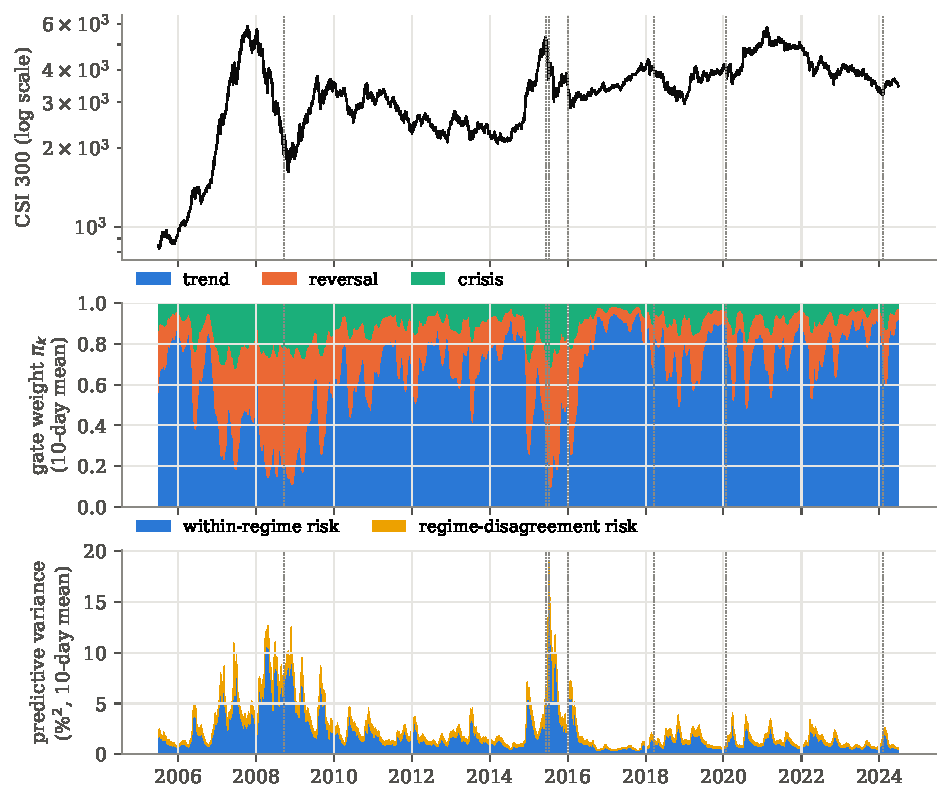
\includegraphics[width=\textwidth]{../results/figures/csi300_gates_risk.pdf}
\caption{CSI 300: price (top), SMoE gate probabilities (middle) and the decomposition of predictive
variance into within-regime and regime-disagreement risk (bottom), in sample. Dotted lines mark the
policy and market events of \cref{tab:events}.}\label{fig:gates}
\end{figure}

\begin{figure}[t]\centering
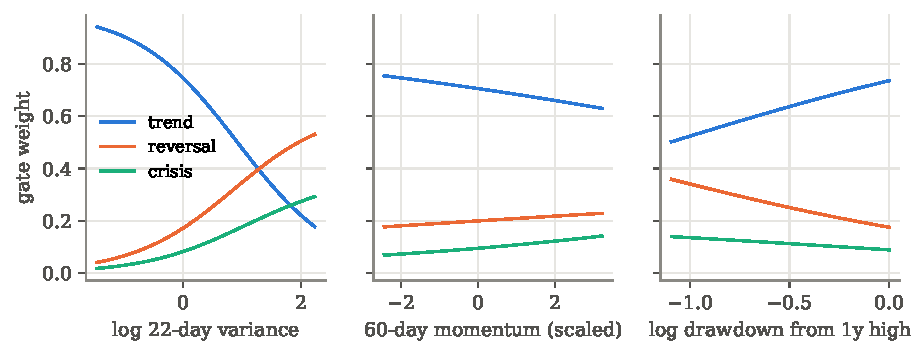
\includegraphics[width=\textwidth]{../results/figures/csi300_gate_curves.pdf}
\caption{Gate response curves for CSI 300: $\pi_k$ as a function of each state variable with the
others at their sample means. Only volatility moves the gate materially, matching the Wald tests.}
\label{fig:gate_curves}
\end{figure}

\subsection{Reading the forecasts}
\Cref{fig:whitebox} applies the closed forms of \cref{sec:whitebox} to the fitted CSI~300 model. The top
panel is the exact attribution \eqref{eq:attr} of the predictive mean to the three experts. The
short-horizon (``reversal'') and crisis experts carry large and opposite contributions that largely
cancel; in the 2008 and 2015 turmoil both widen to about half a percentage point a day. The predictive
\emph{mean} is therefore the small difference of two large regime-specific forecasts. This is a reason to
distrust any single point forecast of the daily return, and seeing it requires a mixture with explicit
components. The middle panel shows the probability of a rise, which exceeds one half on 64\% of
days but rarely departs from it by more than ten percentage points.

The bottom panel is the gate elasticity of the 1\% VaR with respect to the volatility state,
computed in closed form (\cref{app:derivations}). Through the gate alone (holding every expert's mean
and variance fixed) a one-standard-deviation rise in log volatility lowers the 1\% VaR by $0.58$
percentage points on average, with a 5--95\% range of $0.24$ to $0.83$. The effect is weakest in the
middle of the 2008 and 2015 crises, when the gate has already shifted most of its weight away from the
trend expert and has little left to move. Statements of this kind (exact, decomposed by channel and
state-dependent) are what we mean by a white box.

\begin{figure}[t]\centering
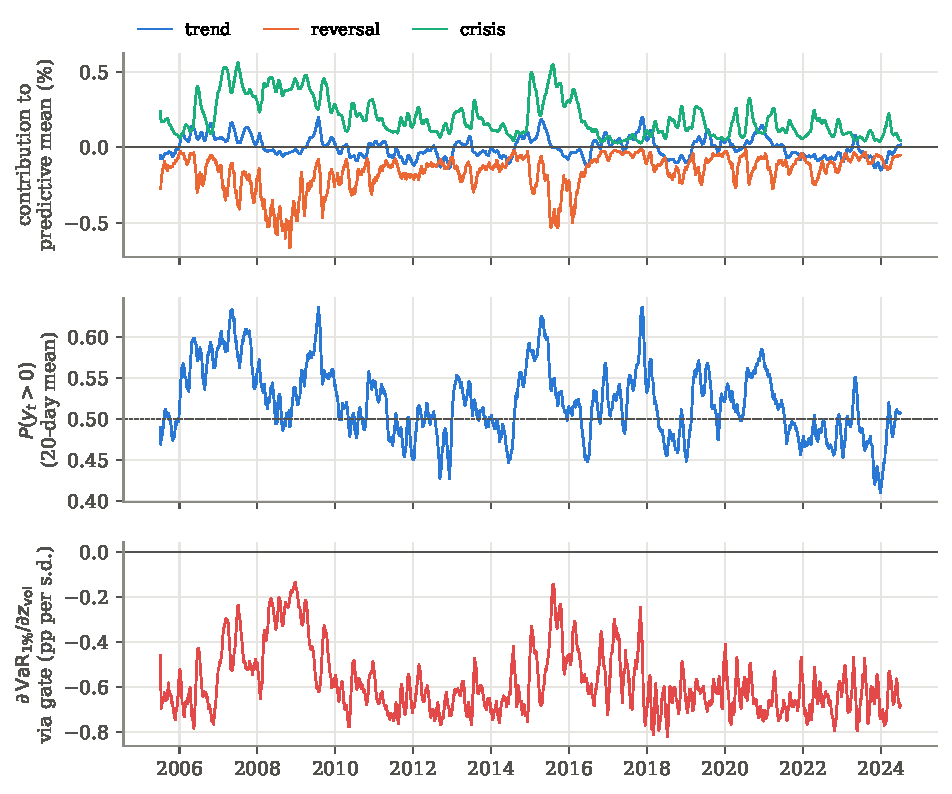
\includegraphics[width=\textwidth]{../results/figures/csi300_whitebox.pdf}
\caption{CSI 300 through the white box (in sample, 20-day averages). Top: exact attribution of the
predictive mean to the experts. Middle: probability of a rise. Bottom: closed-form gate elasticity of
the 1\% VaR with respect to the volatility state, in percentage points per standard deviation.}
\label{fig:whitebox}
\end{figure}

\subsection{Policy and market events}
Because the gate is a function of observables, its reading around known events is a falsifiable
description of what the model does. Around the start of the 2015 crash the 20-day average trend
weight halves (from $0.42$ to $0.21$) while the reversal and crisis weights rise; after the rescue
package of July 2015 the trend weight falls further to $0.11$. The circuit-breaker episode of January
2016 shows the same pattern in smaller magnitude. Two events move the gate the other way or not at
all: the 2018 tariff announcements coincided with a \emph{higher} trend weight (the sell-off was
gradual and low-volatility at first), and the 2008 stamp-duty cut left the weights unchanged. The
gate therefore responds to the change in volatility that an event brings; the headline itself does
not enter. This reading is available only because the gate is a known function of observables.

\subsection{Out-of-sample forecasts}
\Cref{tab:loss_NLL,tab:loss_CRPS,tab:loss_QLIKE,tab:loss_FZ5} report out-of-sample losses for all
models and assets relative to GARCH-$t$. For the Chinese equity series the SMoE ties with the GARCH
family. Its log-score difference from GARCH-$t$ is $-0.002$ (CSI~300), $-0.023$ (CSI~500), $+0.003$
(SSE~50) and $+0.004$ (ChiNext); for CSI~300 it is inside the 10\% model confidence set for all four
losses (MCS $p$-values $0.64$--$0.89$), together with the GARCH models, LSTAR and the deep SMoE.
Models that are \emph{excluded} for CSI~300 are equally informative: the historical Gaussian, the
Markov-switching regression and all three zero-shot foundation models under every loss, the boosted
model under every loss except CRPS, and the single-regime Gauss-HAR for log score.

The variance forecasts can be checked against realised variance from 5-minute data, which is a far
more precise proxy than squared returns. Against $\mathrm{RV}_t+r^2_{\text{overnight},t}$ the SMoE has
the highest Mincer--Zarnowitz $R^2$ of all models ($0.355$, versus $0.244$ for GARCH-$t$) and the
second-lowest MSE. On QLIKE four models are marginally better (LSTAR, Gauss-HAR, the boosted model
and the MAR, $0.293$--$0.299$ against $0.303$), all of which use the same range-based HAR variance
covariates (\cref{tab:rv}).


\begin{table}[!htbp]\centering\scriptsize
\caption{SMoE estimates for CSI 300, January 2005--June 2024}\label{tab:csi300_params}
\begin{adjustbox}{max width=\textwidth}
\begin{tabular}{lrrrrr}
\toprule
Parameter & Estimate & SE (sandwich) & SE (model) & $z$ & $p$\\
\midrule
\texttt{beta[trend]:const} & -0.000 & 0.029 & 0.029 & -0.002 & 0.998\\
\texttt{beta[trend]:mom20} & 0.011 & 0.025 & 0.024 & 0.426 & 0.670\\
\texttt{beta[trend]:mom120} & 0.106 & 0.028 & 0.027 & 3.809 & 0.000\\
\texttt{beta[reversal]:const} & -0.728 & 0.262 & 0.183 & -2.782 & 0.005\\
\texttt{beta[reversal]:rev1} & 0.278 & 0.126 & 0.120 & 2.208 & 0.027\\
\texttt{beta[reversal]:rev5} & 0.184 & 0.166 & 0.125 & 1.104 & 0.269\\
\texttt{beta[crisis]:const} & 1.773 & 0.272 & 0.229 & 6.516 & 0.000\\
\texttt{delta[trend]:const} & -0.219 & 0.120 & 0.093 & -1.833 & 0.067\\
\texttt{delta[trend]:lv1} & 0.054 & 0.070 & 0.064 & 0.769 & 0.442\\
\texttt{delta[trend]:lv5} & 0.012 & 0.115 & 0.104 & 0.107 & 0.915\\
\texttt{delta[trend]:lv22} & 0.376 & 0.115 & 0.108 & 3.270 & 0.001\\
\texttt{delta[reversal]:const} & 1.372 & 0.137 & 0.097 & 10.024 & 0.000\\
\texttt{delta[reversal]:lv1} & 0.226 & 0.087 & 0.088 & 2.591 & 0.010\\
\texttt{delta[reversal]:lv5} & 0.245 & 0.124 & 0.117 & 1.979 & 0.048\\
\texttt{delta[reversal]:lv22} & 0.159 & 0.116 & 0.102 & 1.372 & 0.170\\
\texttt{delta[crisis]:const} & -0.327 & 0.290 & 0.263 & -1.125 & 0.261\\
\texttt{delta[crisis]:lv1} & 0.422 & 0.187 & 0.209 & 2.254 & 0.024\\
\texttt{delta[crisis]:lv5} & 0.065 & 0.235 & 0.272 & 0.274 & 0.784\\
\texttt{delta[crisis]:lv22} & 0.331 & 0.206 & 0.225 & 1.603 & 0.109\\
\texttt{gamma[trend]:const} & 1.970 & 0.407 & 0.339 & 4.845 & 0.000\\
\texttt{gamma[trend]:g\_lvol} & -1.033 & 0.162 & 0.149 & -6.385 & 0.000\\
\texttt{gamma[trend]:g\_mom60} & -0.216 & 0.146 & 0.124 & -1.481 & 0.139\\
\texttt{gamma[trend]:g\_dd} & 0.154 & 0.141 & 0.129 & 1.091 & 0.275\\
\texttt{gamma[reversal]:const} & 0.725 & 0.481 & 0.362 & 1.505 & 0.132\\
\texttt{gamma[reversal]:g\_lvol} & -0.053 & 0.172 & 0.151 & -0.311 & 0.756\\
\texttt{gamma[reversal]:g\_mom60} & -0.112 & 0.203 & 0.157 & -0.549 & 0.583\\
\texttt{gamma[reversal]:g\_dd} & -0.049 & 0.156 & 0.125 & -0.316 & 0.752\\
\bottomrule
\end{tabular}
\end{adjustbox}
\par\smallskip\begin{minipage}{\textwidth}\footnotesize
$z$ and $p$ use the sandwich standard errors with Newey--West meat.
\end{minipage}
\end{table}
\begin{table}[!htbp]\centering\small
\caption{Robust Wald tests of semantic restrictions, CSI 300}\label{tab:csi300_wald}
\begin{adjustbox}{max width=\textwidth}
\begin{tabular}{lrrr}
\toprule
Null hypothesis & Wald & df & $p$\\
\midrule
all gate slopes = 0 (SMoE vs MAR) & 70.812 & 6 & 0.000\\
volatility does not enter the gate & 46.202 & 2 & 0.000\\
momentum does not enter the gate & 3.895 & 2 & 0.143\\
drawdown does not enter the gate & 3.985 & 2 & 0.136\\
trend expert slopes = 0 & 21.561 & 2 & 0.000\\
reversal expert slopes = 0 & 5.616 & 2 & 0.060\\
all mean slopes = 0 & 23.956 & 4 & 0.000\\
equal variance dynamics across experts & 16.034 & 6 & 0.014\\
\bottomrule
\end{tabular}
\end{adjustbox}
\end{table}
\begin{table}[!htbp]\centering\small
\caption{In-sample likelihood comparison, CSI 300}\label{tab:csi300_lik}
\begin{adjustbox}{max width=\textwidth}
\begin{tabular}{lrrrr}
\toprule
model & loglik & params & AIC & BIC\\
\midrule
Gauss-HAR (K=1) & -7993.5 & 9 & 16,005 & 16,063\\
MAR & -7842.0 & 21 & 15,726 & 15,861\\
LSTAR & -7860.3 & 16 & 15,753 & \textbf{15,856}\\
SMoE & -7828.2 & 27 & \textbf{15,710} & 15,884\\
\bottomrule
\end{tabular}
\end{adjustbox}
\end{table}

\section{Results II: nineteen markets}\label{sec:results-global}

\subsection{Density forecasts}
Across the nineteen series the SMoE has the best average rank in log score (2.95 among 13 models),
followed by the deep SMoE (3.3), the MAR (3.5) and AR-GJR-$t$ (3.6). Pairwise, it beats every model
outside the GARCH and mixture families on almost every asset: on log score it is significantly better
(one-sided DM-HLN, 5\%) than the single-regime Gauss-HAR on 17 series, the Markov-switching regression
on 17, the boosted model on 17, and each of the three foundation models on all 19, and it is never
significantly worse than
any of them. Against GARCH-$t$ it is better on 11 of 19 series (significantly on 8; significantly
worse on one, SHFE gold), against the MAR on 14 (5 significant, 2 significantly
worse) and against the deep SMoE on 10 (6 and 2). The model confidence set at 10\% retains the SMoE
for 15 series on log score and 18 on both QLIKE and the FZ0 loss for (VaR, ES).

\begin{figure}[t]\centering
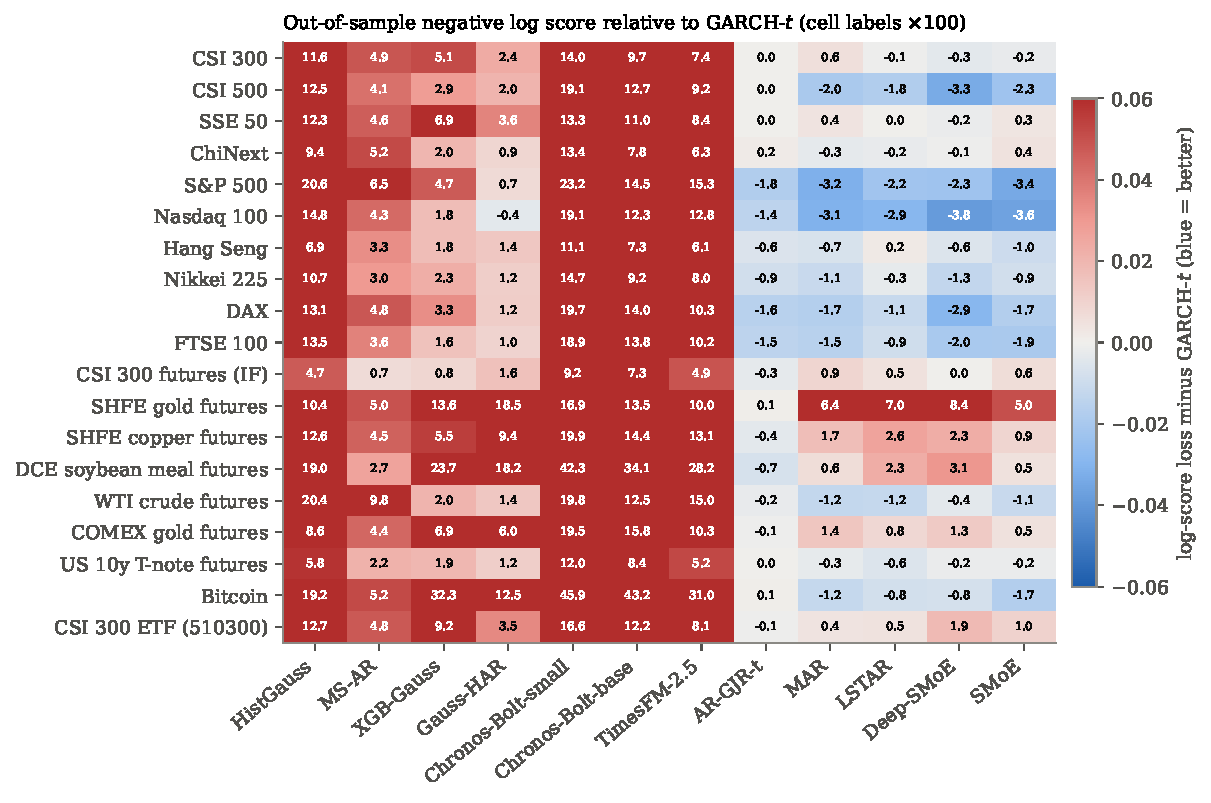
\includegraphics[width=\textwidth]{../results/figures/heatmap_nll.pdf}
\caption{Out-of-sample log-score loss of every model minus that of GARCH-$t$, by series (blue: better
than GARCH-$t$; red: worse; cell labels $\times100$). The two leftmost blocks of columns are dominated
by every mixture model; the SMoE, the MAR, the LSTAR and the deep SMoE are blue on most equity
series.}\label{fig:heatmap}
\end{figure}

We draw two conclusions. First, most of the gain of a mixture over a single Gaussian comes from the
\emph{shape} and \emph{variance dynamics} of the predictive distribution: the constant-weight MAR
already captures much of it, and the observable gate adds a small but frequently significant
increment. Second, the white-box SMoE is statistically indistinguishable from its black-box
counterpart in most markets, a finding we make precise with the yardstick in \cref{sec:yardstick}.

\subsection{Which parts of the SMoE matter?}
\Cref{tab:ablation} removes one component at a time and re-runs the walk-forward on eight series.
The components rank clearly. Removing the variance dynamics (constant expert variances) does the most
damage: the full model is significantly better on log score for six of eight
series and on QLIKE for seven, and never worse. Dropping the short-horizon expert ($K=2$) costs log
score significantly on four series and improves it on one. Removing the semantic exclusion restrictions (letting every expert see every
covariate) never improves log score and worsens it on three series: the restrictions buy
identification and interpretability at no predictive cost. Finally, a gate driven by volatility alone
is statistically indistinguishable from the full three-variable gate, in line with the in-sample Wald
tests; a parsimonious practitioner would use it.

\begin{table}[!htbp]\centering\small
\caption{Out-of-sample ablations of the SMoE on eight series (variant minus full model; positive = variant worse)}\label{tab:ablation}
\begin{adjustbox}{max width=\textwidth}
\begin{tabular}{llrrr}
\toprule
Variant & Loss & Median loss difference & Full SMoE significantly better & Full SMoE significantly worse\\
\midrule
SMoE-K2 & CRPS & -0.0002 & 1 & 0\\
SMoE-K2 & FZ5 & 0.0059 & 2 & 0\\
SMoE-K2 & NLL & 0.0039 & 4 & 1\\
SMoE-K2 & QLIKE & 0.0027 & 3 & 1\\
SMoE-constvar & CRPS & 0.0044 & 4 & 0\\
SMoE-constvar & FZ5 & 0.0210 & 4 & 0\\
SMoE-constvar & NLL & 0.0161 & 6 & 0\\
SMoE-constvar & QLIKE & 0.0369 & 7 & 0\\
SMoE-unrestricted & CRPS & 0.0004 & 1 & 1\\
SMoE-unrestricted & FZ5 & -0.0037 & 1 & 0\\
SMoE-unrestricted & NLL & 0.0031 & 3 & 0\\
SMoE-unrestricted & QLIKE & -0.0024 & 1 & 0\\
SMoE-volgate & CRPS & -0.0000 & 1 & 0\\
SMoE-volgate & FZ5 & -0.0034 & 1 & 2\\
SMoE-volgate & NLL & 0.0025 & 1 & 0\\
SMoE-volgate & QLIKE & -0.0019 & 2 & 1\\
\bottomrule
\end{tabular}
\end{adjustbox}
\par\smallskip\begin{minipage}{\textwidth}\footnotesize
Series: CSI 300, CSI 500, SSE 50, ChiNext, S\&P 500, Hang Seng, COMEX gold, Bitcoin. Counts of series with one-sided DM-HLN $p<0.05$ in favour of the full model and two-sided $p<0.05$ against it.
\end{minipage}
\end{table}

\subsection{Means and directions}
Consistent with \cref{sec:lagging} and with \citet{welch2008comprehensive}, no model forecasts daily
means reliably. The median out-of-sample $R^2$ against a zero forecast is negative for every model,
between $-0.07\%$ (AR-GJR-$t$) and $-2.3\%$ (TimesFM-2.5). The Clark--West test rejects at 5\% for the SMoE on three series (S\&P~500,
Nasdaq~100, DCE soybean meal) and the hit rate averages $50.9\%$. On squared error and Brier score the
simplest models rank best. In daily data, a distributional model earns its keep in risk forecasts;
it does not forecast direction.


\subsection{Calibration}
Calibration is where the SMoE separates from the GARCH family. Its 1\% VaR passes the Kupiec test on
17 of 19 series (GARCH-$t$: 10; historical Gaussian: 1) and its average 1\% violation rate is
$0.97\%$. At 5\% the SMoE is slightly conservative (average violation rate $4.2\%$), which the
conformal layer corrects (\cref{sec:conformal-results}). The PIT standard deviation is $0.97$, close to
the ideal of one. The Chronos-Bolt models have average PIT standard deviations of $1.25$ and $1.32$,
i.e.\ their predictive distributions are far too narrow, which explains their poor log scores
(\cref{fig:pit}). TimesFM~2.5 is better calibrated ($1.17$) but still too narrow: its 1\% VaR is
violated on $3.1\%$ of days on average and fails the Kupiec test on every series, as do both
Chronos models.


\begin{figure}[t]\centering
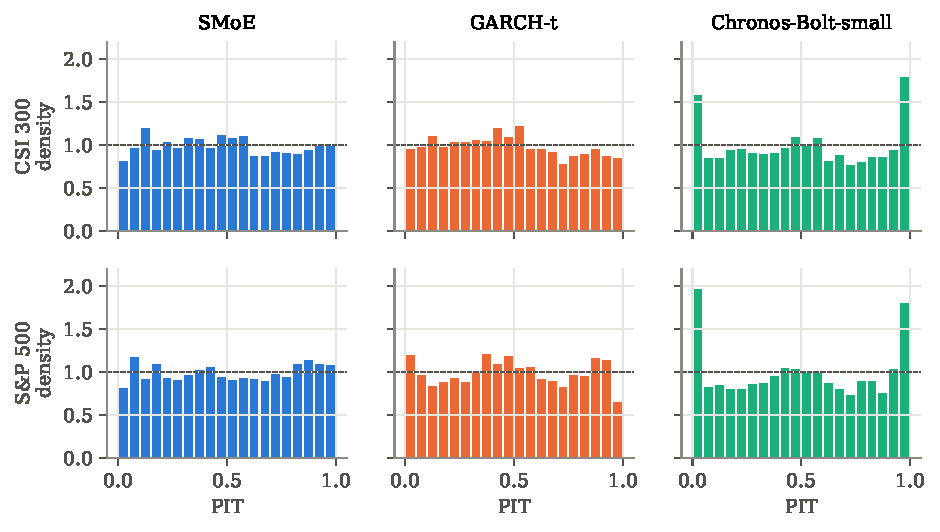
\includegraphics[width=\textwidth]{../results/figures/pit_hist.pdf}
\caption{Probability integral transforms of out-of-sample forecasts. A calibrated forecaster has a
flat histogram (dashed line). The foundation model's U shape shows predictive distributions that are
too narrow.}\label{fig:pit}
\end{figure}

\subsection{Cross-market white-box fingerprints}
\Cref{tab:fingerprints} collects the key SMoE coefficients for every series and
\cref{fig:fingerprints} plots their robust $t$-statistics.

\begin{figure}[t]\centering
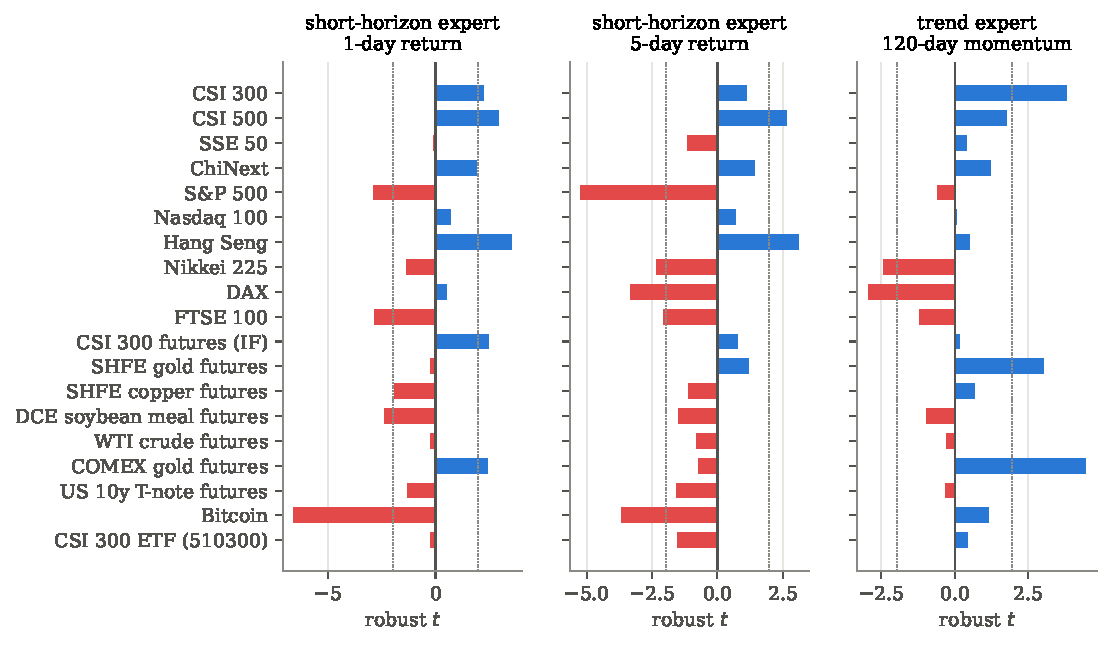
\includegraphics[width=\textwidth]{../results/figures/fingerprints.pdf}
\caption{White-box fingerprints: robust $t$-statistics of the short-horizon expert's loadings on the
scaled 1- and 5-day returns and of the trend expert's loading on 120-day momentum, by series. Dotted
lines mark $\pm1.96$.}\label{fig:fingerprints}
\end{figure} The pattern of the
short-horizon expert is the clearest cross-market regularity in the paper. In the Chinese equity
indices the scaled one-day return enters with a \emph{positive} sign (CSI~300 $z=2.2$, CSI~500
$z=2.9$, ChiNext $z=1.9$), while the five-day scaled return is \emph{negative} and highly significant
in the S\&P~500 ($z=-5.2$), the DAX ($z=-3.3$), the Nikkei ($z=-2.3$) and the FTSE ($z=-2.1$).
Short-horizon continuation in China and short-horizon reversal in developed markets is consistent with
the dominance of retail order flow in the A-share market \citep{liu2019size}; in the SMoE it is not an
unconditional autocorrelation but a property of a specific, high-variance regime, with a
standard error. Slow momentum is equally market-specific: 120-day momentum enters the trend expert
positively and significantly for CSI~300 ($z=3.8$) and both gold contracts ($z=3.0$ and $4.5$), but
negatively for the Nikkei and the DAX ($z=-2.4$ and $-3.0$), where the trend regime is better
described by 20-day momentum.

\section{Results III: how many experts, and what drives the gate?}\label{sec:kgate}

The SMoE of \cref{sec:model} fixes $K=3$ and a three-variable gate by semantic design. A
referee is entitled to ask whether either choice is supported by the data. This section answers
with a systematic comparison: six alternative expert sets ($K=1,\dots,5$), five alternative gates,
in-sample information criteria, a parametric bootstrap of the likelihood ratio, and a score test that
screens candidate state variables from the baseline fit alone. Three theoretical points come first,
because the usual tools do not apply directly.

\subsection{Theory}

\paragraph{Experts that share a semantic group.}
Two of the larger specifications add a second intercept-only expert, which shares the empty
covariate set with the crisis expert and therefore violates \cref{ass:ident}(c). Identification
then has to come from the variance functions.

\begin{proposition}[Identification with a shared semantic group]\label{prop:ident-shared}
Let \cref{ass:ident}(a)--(b) hold and let (c) hold for every pair of experts with different
mean-covariate sets. If experts $k$ and $l$ share a covariate set, assume $\delta_{k,0}\neq\delta_{l,0}$
and adopt the labelling convention $\delta_{k,0}<\delta_{l,0}$ (expert $k$ is the calmer one). Then
$p_{\btheta}=p_{\btheta'}$ almost everywhere implies $\btheta=\btheta'$.
\end{proposition}

\noindent The proof (\cref{app:proofs}) repeats the argument for \cref{prop:ident} up to the
constant permutation $\varsigma$, which can now only exchange experts within a shared group; the
convention rules out the exchange. In practice the convention is imposed after estimation by
relabelling, and it does not affect any predictive quantity.

\paragraph{Testing $K$.}
Testing $K-1$ against $K$ experts is a boundary problem with unidentified nuisance parameters. The
null is reached either when the extra expert's gate weight vanishes ($\gamma_{K,0}\to-\infty$, so its
mean and variance parameters are not identified) or when the extra expert coincides with an
existing one (so the gate parameters separating them are not identified). In either case the
information matrix is singular at the null and the likelihood ratio has no $\chi^2$ limit; for
normal mixtures it may even diverge slowly \citep{hartigan1985failure,chen2001modified}. We therefore
use three tools that do not rely on a $\chi^2$ limit. The first is out-of-sample log score, which is
what the paper is about. The second is BIC, $-2\ell_n(\hat\btheta)+\dim(\btheta)\log n$, which is a
Laplace approximation to the log marginal likelihood \citep{schwarz1978estimating} and selects the
order of a mixture consistently under conditions given by \citet{keribin2000consistent}. The third
is the fixed-design parametric bootstrap of \citet{mclachlan1987bootstrapping}: hold the covariates
at their observed values, draw $y^\ast_t$ from the fitted null model, re-estimate both models on
$y^\ast$, and compare the observed LR statistic with the bootstrap distribution. The bootstrap
treats the covariates as fixed although they are functions of past returns; this is the standard
conditional version of the test and it is conservative when the alternative improves the fit of
the covariates' own dynamics, which the SMoE does not model.

\paragraph{Screening gate variables with a score test.}
Adding a state variable $\bm w_t\in\R^d$ to the gate changes the log-odds to
$\bm\gamma_k^\top\tilde\bz_t+\bm\psi_k^\top\bm w_t$. Under $H_0:\bm\psi=\bm 0$ the number of
experts is unchanged, all parameters stay identified, and standard theory applies. The score test
is especially convenient here because Fisher's identity \eqref{eq:score} gives the new scores in
closed form at the restricted estimate.

\begin{proposition}[LM test for omitted gate variables]\label{prop:lm-gate}
Let $\hat\btheta$ be the QMLE of the SMoE with gate covariates $\bz_t$, and let the augmented model
with gate covariates $(\bz_t,\bm w_t)$ satisfy \cref{ass:ident,ass:asym} at its pseudo-true value
$(\btheta^\ast,\bm\psi^\ast)$. The score of $\bm\psi_k$ at $(\hat\btheta,\bm0)$ is
\begin{equation}\label{eq:lm-score}
  \bm s_{\psi_k}=\sum_{t=1}^n\big(\hat\tau_{tk}-\hat\pi_{tk}\big)\,\bm w_t,\qquad k=1,\dots,K-1,
\end{equation}
the covariance between the candidate variable and the regime surprise, the gap between posterior
and prior regime probabilities. Let $\bm s$ stack all scores of the augmented model at
$(\hat\btheta,\bm0)$, partition $A$ and $B$ conformably into the $\btheta$ and $\bm\psi$ blocks, and set
$C=[-A_{\psi\theta}A_{\theta\theta}^{-1},\;I]$. Then under $H_0:\bm\psi^\ast=\bm0$
\begin{equation}\label{eq:lm}
  \mathrm{LM}=(C\bm s)^\top\big(C\hat BC^\top\big)^{-1}(C\bm s)\;\xrightarrow{d}\;\chi^2_{(K-1)d},
\end{equation}
with $\hat A,\hat B$ the Hessian and Newey--West estimators of \cref{sec:estimation}. Under local
alternatives $\bm\psi^\ast=\bm h/\sqrt n$, $\mathrm{LM}$ and the robust Wald statistic from the
augmented fit have the same non-central $\chi^2$ limit.
\end{proposition}

\noindent The test needs only the baseline fit, so a list of candidate state variables can be
screened at the cost of one estimation. It also has a direct white-box reading: a state variable
belongs in the gate if it predicts the regime surprise $\tau_{tk}-\pi_{tk}$, i.e.\ if the data assign
days to regime $k$ more (or less) often than the gate expected whenever $\bm w_t$ is high. This is a
conditional moment test in the sense of \citet{newey1985maximum} and \citet{tauchen1985diagnostic},
applied to the latent regime label. The correction $C$ matters: the restricted parameters are
estimated, and the uncorrected statistic $\bm s_\psi^\top\hat B_{\psi\psi}^{-1}\bm s_\psi$ is not
$\chi^2$ under the null.

\subsection{Design}

\Cref{tab:kg-design} lists the specifications. Along the $K$ dimension we drop either of the two
covariate experts or the crisis expert ($K=2$), add a second intercept-only ``calm'' expert, a
``premium'' expert whose mean depends on the log 22-day variance and the drawdown ($K=4$), or both
($K=5$). The premium expert gives the risk--return trade-off of \citet{french1987expected} a regime of
its own: if expected returns rise with variance in some states, its variance loading is positive.
Along the gate dimension we use volatility alone, add the log VIX of the previous US trading day
\citep{whaley2000investor,bekaert2014vix}, add the signed last return (an asymmetric gate that can
react differently to up and down days), or add all three of VIX, last return and the log one-day
range variance. The VIX enters with a one-day lag for every series, so it is known at the local
close in every time zone (\cref{app:leakage}). All specifications are estimated in the same
walk-forward on all nineteen series.

\begin{table}[t]\centering\small
\caption{Specifications compared in \cref{sec:kgate}}\label{tab:kg-design}
\begin{adjustbox}{max width=\textwidth}\begin{tabular}{llll}\toprule
Name & $K$ & Experts (mean covariates) & Gate covariates\\\midrule
Gauss-HAR & 1 & single (trend + short-horizon) & --\\
SMoE-K2tc & 2 & trend; crisis & baseline\\
SMoE-K2rc & 2 & short-horizon; crisis & baseline\\
SMoE-K2tr & 2 & trend; short-horizon & baseline\\
LSTAR & 2 & trend; short-horizon & log 22d variance\\
\textbf{SMoE} & 3 & trend; short-horizon; crisis & baseline\\
MAR & 3 & as SMoE & constant\\
SMoE-K4c & 4 & + calm (intercept only) & baseline\\
SMoE-K4p & 4 & + premium (log 22d variance, drawdown) & baseline\\
SMoE-K5 & 5 & + calm + premium & baseline\\
SMoE-Gvol & 3 & as SMoE & log 22d variance\\
SMoE-Gvix & 3 & as SMoE & baseline + log VIX$_{t-1}$\\
SMoE-Gasym & 3 & as SMoE & baseline + $r_t/\hat\sigma_t$\\
SMoE-Grich & 3 & as SMoE & baseline + VIX + $r_t/\hat\sigma_t$ + log 1d variance\\
\bottomrule\end{tabular}\end{adjustbox}
\par\smallskip\footnotesize Baseline gate: log 22-day variance, 60-day scaled momentum, drawdown
from the 250-day high.
\end{table}

\subsection{Out of sample, three experts are right}

\Cref{tab:kg-oos} and \cref{fig:kg} summarise the walk-forward comparison. Along the $K$ dimension the
baseline is best. Every $K=2$ specification is significantly worse than the SMoE in log score on four
to seven series and significantly better on one; the median loss difference is $0.28$ to $0.51$
hundredths of a nat per day. Adding experts does not help either: the calm expert ($K=4$) is never
significantly better and is worse on three series, the premium expert is better on two and worse on
five, and the five-expert model is better on two and worse on nine. The single-regime Gauss-HAR is
worse on 17 of 19
series. Out-of-sample log score therefore traces an inverted U in $K$ with its maximum at three, the
number chosen by semantic design before any data were seen. The larger models also calibrate worse:
their 1\% VaR passes the Kupiec test on 13 to 15 series, against 17 for the SMoE.

Along the gate dimension one change helps. Adding the previous day's log VIX gives the best average
rank on all four losses (log score $3.26$ against $4.79$ for the SMoE, among fourteen
specifications), a lower log score than the SMoE on 13 of 19 series (significantly lower on three and
significantly higher on one), and membership of the 10\% model confidence set on all nineteen. The gain is small: the median
improvement is $0.14$ hundredths of a nat per day. A volatility-only gate is slightly worse than the
three-variable gate (significantly on three series), the asymmetric gate that adds the signed last
return is significantly different from it on only one series, and the constant-weight MAR is
significantly worse on five
series. The largest gate (VIX, last return and one-day variance) is no better than the gate with VIX
alone.

\begin{figure}[t]\centering
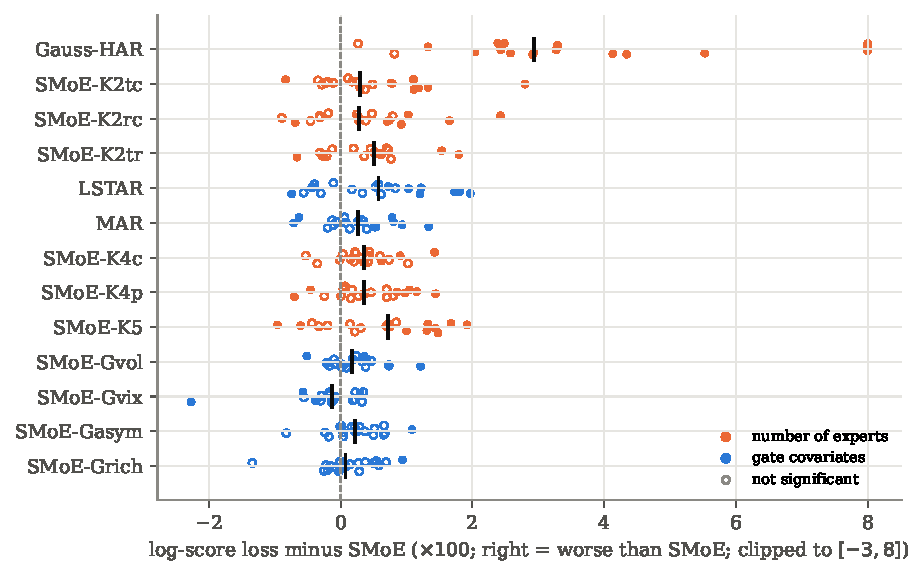
\includegraphics[width=0.92\textwidth]{../results/figures/kg_strip.pdf}
\caption{Out-of-sample log-score loss of each specification minus that of the SMoE, one point per
series (filled: DM-HLN test significant at 5\%, in either direction; vertical bars: medians). Orange:
specifications that change the experts; blue: specifications that change only the gate (LSTAR also
has $K=2$).}\label{fig:kg}
\end{figure}

\begin{table}[!htbp]\centering\footnotesize
\caption{Number of experts and gate covariates: out-of-sample comparison on 19 series (development period)}\label{tab:kg-oos}
\begin{adjustbox}{max width=\textwidth}
\begin{tabular}{lrrrrrrrrrr}
\toprule
Model & $K$ & Rank NLL & Rank CRPS & Rank QLIKE & Rank FZ5 & NLL better & NLL worse & MCS NLL & MCS QLIKE & Kupiec 1\%\\
\midrule
Gauss-HAR & 1 & 13.68 & 12.89 & 8.84 & 10.32 & 0 & 17 & 3 & 11 & 4\\
SMoE-K2tc & 2 & 7.95 & 7.53 & 9.16 & 7.32 & 1 & 7 & 15 & 14 & 17\\
SMoE-K2rc & 2 & 7.26 & 6.79 & 7.21 & 6.84 & 1 & 6 & 15 & 14 & 17\\
SMoE-K2tr & 2 & 8.42 & 8.47 & 7.74 & 6.63 & 1 & 4 & 15 & 15 & 17\\
LSTAR & 2 & 8.42 & 9.16 & 7.95 & 7.32 & 1 & 7 & 13 & 14 & 15\\
SMoE & 3 & 4.79 & 5.79 & 7.16 & 8.00 & -- & -- & 18 & 16 & 17\\
MAR & 3 & 6.74 & 5.74 & 6.89 & 7.05 & 2 & 5 & 16 & 17 & 16\\
SMoE-K4c & 4 & 7.63 & 7.16 & 7.32 & 8.47 & 0 & 3 & 18 & 17 & 14\\
SMoE-K4p & 4 & 8.05 & 8.68 & 6.21 & 8.16 & 2 & 5 & 17 & 17 & 13\\
SMoE-K5 & 5 & 9.05 & 8.68 & 7.26 & 8.68 & 2 & 9 & 17 & 17 & 15\\
SMoE-Gvol & 3 & 6.79 & 7.00 & 6.95 & 6.53 & 1 & 3 & 17 & 16 & 15\\
SMoE-Gvix & 3 & 3.26 & 5.16 & 5.84 & 5.63 & 3 & 1 & 19 & 17 & 16\\
SMoE-Gasym & 3 & 7.11 & 6.11 & 8.74 & 7.79 & 0 & 1 & 18 & 15 & 15\\
SMoE-Grich & 3 & 5.84 & 5.84 & 7.74 & 6.26 & 0 & 1 & 19 & 17 & 16\\
\bottomrule
\end{tabular}
\end{adjustbox}
\par\smallskip\begin{minipage}{\textwidth}\footnotesize
Average ranks among the 14 specifications (1 = best). NLL better/worse: series on which the specification is significantly better (one-sided DM-HLN, 5\%) or worse (two-sided, 5\%) than the SMoE in log score. MCS: series (of 19) on which the specification is in the 10\% model confidence set of the 14. Kupiec 1\%: series on which the 1\% VaR passes at 5\%.
\end{minipage}
\end{table}

\subsection{In sample, the criteria disagree}

In-sample information criteria point in opposite directions (\cref{tab:kg-bic}). Among the
specifications that differ in $K$, BIC selects two experts on 14 of 19 series and three on five; AIC
selects the five-expert model on nine series. The baseline SMoE is never the BIC choice among all fourteen
specifications, where the VIX gate is selected most often (five series). With three to five thousand
observations, BIC's penalty of $\log n\approx8$ per parameter outweighs the improvements in fit that
the walk-forward rewards, while AIC's penalty of two lets the larger models fit noise that does not
survive out of sample. Neither criterion is a reliable guide to forecasting performance here, which is
a further reason to choose $K$ by out-of-sample log score.

The parametric bootstrap makes the same point from a different angle (\cref{tab:kg-boot}). For the
CSI~300 and the S\&P~500 we test $K=1$ against $K=3$ with 199 draws and $K=3$ against $K=4$ (the
calm expert) with 99. The bootstrap null distributions are far to the right of the naive $\chi^2$
limits: for $K=1$ against $K=3$ the 95\% critical values are $39.2$ and $39.2$, against $28.9$ for a
$\chi^2_{18}$, and for $K=3$ against $K=4$ they are $24.6$ and $21.1$, against $16.9$ for a
$\chi^2_9$. This is the non-regularity described above, and a $\chi^2$ reference would over-reject.
Even against the bootstrap, both tests reject: the single regime with LR statistics of $317$ and $400$
($p=0.005$, the smallest attainable with 199 draws), and three experts in favour of four with
$62.0$ ($p=0.010$) and $43.6$ ($p=0.020$). In sample, a fourth expert is therefore supported;
out of sample, the same four-expert model is never significantly better than the SMoE and is worse
on three series. The likelihood ratio detects a fourth regime that is real in sample but does not
generalise across quarterly re-estimations.

\begin{table}[!htbp]\centering\small
\caption{Parametric bootstrap of the likelihood-ratio test for the number of experts}\label{tab:kg-boot}
\begin{adjustbox}{max width=\textwidth}
\begin{tabular}{lrrrrrr}
\toprule
Series & Test & LR & $B$ & Bootstrap 95\% crit. & Bootstrap mean & $p$\\
\midrule
CSI 300 & K1 vs K3 & 317.152 & 199 & 39.225 & 27.129 & 0.005\\
CSI 300 & K3 vs K4 & 62.018 & 99 & 24.568 & 14.494 & 0.010\\
S\&P 500 & K1 vs K3 & 399.651 & 199 & 39.186 & 25.977 & 0.005\\
S\&P 500 & K3 vs K4 & 43.622 & 99 & 21.111 & 14.010 & 0.020\\
\bottomrule
\end{tabular}
\end{adjustbox}
\par\smallskip\begin{minipage}{\textwidth}\footnotesize
Fixed-design parametric bootstrap \citep{mclachlan1987bootstrapping}: $y^\ast$ drawn from the fitted null model at the observed covariates; both models re-estimated on every draw (best of a warm start and two random starts). $p=(1+\#\{LR^\ast\ge LR\})/(1+B)$. The observed LR uses the same estimation procedure as the draws; the four-start fit of \cref{tab:csi300_lik} gives a slightly larger LR for the CSI 300 ($K=1$ against $K=3$).
\end{minipage}
\end{table}

\begin{table}[!htbp]\centering\footnotesize
\caption{In-sample model selection by BIC (development sample)}\label{tab:kg-bic}
\begin{adjustbox}{max width=\textwidth}
\begin{tabular}{lrrr}
\toprule
Asset & BIC-best (all 14) & BIC-best $K$-spec. & $\Delta$BIC SMoE\\
\midrule
SHFE gold futures & SMoE-Gvix & SMoE-K2rc & 107.3\\
Bitcoin & MAR & SMoE & 24.0\\
ChiNext & LSTAR & SMoE-K2rc & 37.9\\
WTI crude futures & SMoE-K2rc & SMoE-K2rc & 53.4\\
CSI 300 & SMoE-Gasym & SMoE-K2tc & 46.1\\
CSI 500 & SMoE-Gvol & SMoE & 13.9\\
SHFE copper futures & SMoE-Gvix & SMoE-K2tr & 10.6\\
DAX & SMoE-Gasym & SMoE-K2tr & 27.0\\
CSI 300 ETF (510300) & LSTAR & SMoE-K2tc & 50.7\\
FTSE 100 & SMoE-Grich & SMoE-K2tc & 35.3\\
COMEX gold futures & SMoE-Gvix & SMoE-K2tc & 20.5\\
Hang Seng & SMoE-K2rc & SMoE-K2rc & 15.5\\
CSI 300 futures (IF) & LSTAR & SMoE-K2rc & 60.3\\
DCE soybean meal futures & SMoE-Gvol & SMoE & 26.0\\
Nikkei 225 & SMoE-Gvix & SMoE & 23.7\\
Nasdaq 100 & SMoE-Grich & SMoE-K2rc & 45.6\\
S\&P 500 & SMoE-Gvix & SMoE & 40.4\\
SSE 50 & LSTAR & SMoE-K2tc & 45.9\\
US 10y T-note futures & SMoE-K2rc & SMoE-K2rc & 63.9\\
\bottomrule
\end{tabular}
\end{adjustbox}
\par\smallskip\begin{minipage}{\textwidth}\footnotesize
$\Delta$BIC SMoE: BIC of the baseline SMoE minus the smallest BIC (0 when the SMoE is selected).
\end{minipage}
\end{table}

\subsection{Which state variables belong in the gate?}

\Cref{tab:kg-lm} screens three candidates with the score test of \cref{prop:lm-gate}, computed from
the baseline fit alone. The VIX is rejected as irrelevant on 11 of 19 series, the signed last return
on six and the one-day variance on two. The robust Wald test from the augmented VIX fit rejects on
twelve, and the two statistics are of the same size series by series (for the S\&P~500, $37.6$ and
$46.3$ with two degrees of freedom; for SHFE gold, $36.8$ and $49.1$), as the proposition predicts
when the effect is real.

The VIX result is geographically structured. By the robust Wald test at 5\%, the US fear gauge
enters the gate of all five developed equity indices, the Hang Seng, both gold contracts, WTI crude
and soybean meal, but not that of the CSI~300 ($p=0.06$), the CSI~500, ChiNext, the IF futures,
copper, the T-note or Bitcoin. Among the A-share series only the SSE~50 and, marginally, the CSI~300
ETF ($p=0.037$, on a sample that starts in 2012) respond.
 In the developed equity indices the sign is uniform: at a given level of the index's
own 22-day variance, a higher VIX moves weight from the crisis expert to the two covariate experts
($z$ between $1.8$ and $6.0$). The VIX is forward-looking while the range-based state is not, so
conditional on recent realised variance a high VIX appears to signal risk that the trend and
short-horizon regimes, with their own variance dynamics, can carry. For the A-share market, the
absence of a VIX effect is consistent with its partial segmentation from global risk appetite. For
the CSI~300 the score test instead flags the most recent day: the one-day variance ($p=0.004$) and the
signed last return ($p=0.033$) are both rejected as irrelevant, so regime weights in the Chinese
index respond to yesterday's move as well as to the 22-day variance.

The premium expert does not find a risk--return trade-off. Its loading on the log 22-day variance is
positive and significant only for the CSI~500 and WTI and negative and significant for the CSI~300
and the SSE~50. Its loading on the drawdown state, by contrast, is negative and significant on seven
series (four Chinese equity indices, the FTSE, SHFE gold and the T-note). Because the drawdown state
$\log(P_t/\max_{j<250}P_{t-j})$ is non-positive, a negative loading means a higher expected return
deep in a drawdown. The fourth expert, given the chance, describes rebounds after large losses rather
than compensation for variance.

\begin{table}[!htbp]\centering\footnotesize
\caption{Screening gate variables: robust LM $p$-values from the baseline fit (\cref{prop:lm-gate}), development sample}\label{tab:kg-lm}
\begin{adjustbox}{max width=\textwidth}
\begin{tabular}{lrrrrrr}
\toprule
Asset & LM: VIX & LM: return & LM: 1d var. & LM: all three & Wald VIX $p$ & premium: $\beta_{\mathrm{lv22}}$ ($z$)\\
\midrule
CSI 300 & 0.083 & 0.033 & 0.004 & 0.003 & 0.060 & -0.950 (-2.8)\\
CSI 500 & 0.512 & 0.224 & 0.039 & 0.005 & 0.252 & 0.485 (4.6)\\
SSE 50 & 0.003 & 0.018 & 0.853 & 0.000 & 0.000 & -0.890 (-2.0)\\
ChiNext & 0.385 & 0.822 & 0.493 & 0.739 & 0.421 & 0.351 (1.2)\\
S\&P 500 & 0.000 & 0.081 & 0.205 & 0.000 & 0.000 & -0.576 (-0.2)\\
Nasdaq 100 & 0.000 & 0.000 & 0.957 & 0.000 & 0.000 & 0.010 (0.3)\\
Hang Seng & 0.009 & 0.337 & 0.141 & 0.010 & 0.001 & -0.136 (-0.7)\\
Nikkei 225 & 0.000 & 0.013 & 0.508 & 0.000 & 0.000 & 0.154 (0.5)\\
DAX & 0.027 & 0.002 & 0.377 & 0.004 & 0.017 & 0.290 (0.4)\\
FTSE 100 & 0.000 & 0.000 & 0.070 & 0.000 & 0.000 & 0.143 (1.1)\\
CSI 300 futures (IF) & 0.181 & 0.167 & 0.738 & 0.236 & 0.074 & 0.014 (0.1)\\
SHFE gold futures & 0.000 & 0.464 & 0.840 & 0.000 & 0.000 & -0.072 (-1.6)\\
SHFE copper futures & 0.189 & 0.139 & 0.191 & 0.120 & 0.051 & 0.067 (0.9)\\
DCE soybean meal futures & 0.001 & 0.233 & 0.708 & 0.004 & 0.000 & 0.059 (1.0)\\
WTI crude futures & 0.008 & 0.274 & 0.709 & 0.066 & 0.040 & 0.284 (2.3)\\
COMEX gold futures & 0.000 & 0.510 & 0.328 & 0.000 & 0.000 & 0.040 (0.5)\\
US 10y T-note futures & 0.385 & 0.171 & 0.565 & 0.235 & 0.165 & 0.103 (1.2)\\
Bitcoin & 0.510 & 0.963 & 0.154 & 0.460 & 0.587 & 0.110 (0.6)\\
CSI 300 ETF (510300) & 0.052 & 0.069 & 0.529 & 0.056 & 0.037 & -0.329 (-1.1)\\
\bottomrule
\end{tabular}
\end{adjustbox}
\par\smallskip\begin{minipage}{\textwidth}\footnotesize
LM: $p$-value of the score test that the candidate is absent from the gate, computed from the baseline SMoE alone ($2d$ df). Wald VIX $p$: robust Wald test of the same hypothesis for VIX from the augmented fit (SMoE-Gvix). Premium: standardised loading of the premium expert's mean on log 22-day variance in SMoE-K4p, with robust $z$-statistic.
\end{minipage}
\end{table}

\paragraph{Summary.} Three experts are supported out of sample. In sample, BIC prefers fewer and the
bootstrapped likelihood ratio prefers more, and neither choice forecasts better. The three-variable gate is a reasonable default, and the VIX is the only
addition that both passes the score test on most series and improves out-of-sample forecasts. Because
we made these comparisons on the development sample after the main specification was fixed, the
lockbox results of \cref{sec:lockbox} still refer to the original SMoE.

\section{Results IV: variance features from 5-minute data}\label{sec:rv}

The SMoE's variance covariates are built from the daily high--low range because the range is
available for every series and every day. For the CSI~300 we also have 5-minute bars, and realised
variance from intraday returns is the textbook measure of daily variance
\citep{andersen2003modeling}. This section asks whether the conclusions change when the range is
replaced by realised measures, and it turns the comparison into a test of a measurement-error
prediction that the white box makes possible.

\subsection{Theory: what a better variance measure should change}

Let $\ell_t=\log\sigma^2_t$ denote the latent log variance of day $t$'s trading session. Every daily
estimator we use has the multiplicative form $\hat v_t=\sigma^2_t\varepsilon_t$, so
\begin{equation}\label{eq:logmeas}
  \log\hat v_t=\ell_t+\kappa+\eta_t,\qquad \E\eta_t=0,\quad \Var\eta_t=\omega^2,
\end{equation}
with $\eta_t$ independent of $\{\ell_s\}$. Under a Brownian semimartingale with constant intraday
volatility and no microstructure noise, $\varepsilon_t$ has a known law. For the squared daily
return $\varepsilon_t\sim\chi^2_1$ and $\omega^2=\psi'(1/2)=\pi^2/2\approx4.93$, where $\psi'$ is the
trigamma function. For realised variance from $M$ intraday returns
$\varepsilon_t\sim\chi^2_M/M$, so $\kappa=\psi(M/2)-\log(M/2)$ and $\omega^2=\psi'(M/2)\approx2/M$;
with $M=48$ five-minute returns, $\omega^2=0.043$. For the Parkinson estimator $\varepsilon_t$ is the
squared range of a standard Brownian motion on $[0,1]$ divided by $4\log2$; its log-variance has no
simple closed form and we compute it by simulation (\cref{tab:rv-measure}). Microstructure noise and
the intraday volatility pattern raise the effective $\omega^2$ of both intraday estimators
\citep{hansen2006realized}, which is why we also estimate it from the data.

\paragraph{What a log-variance error costs.}
The cost of a variance error in log score has a simple exact form.

\begin{lemma}[Cost of a log-variance error]\label{lem:logvar-cost}
Let $y\sim\N(\mu,\sigma^2)$ and let the forecast be $\N(\mu,s^2)$ with $u=\log(s^2/\sigma^2)$. Then
\begin{equation}\label{eq:logvar-cost}
  \E\big[-\log\varphi(y;\mu,s^2)\big]-\E\big[-\log\varphi(y;\mu,\sigma^2)\big]=\tfrac12\big(u+e^{-u}-1\big)
  =\tfrac{u^2}{4}-\tfrac{u^3}{12}+O(u^4),
\end{equation}
which is one half of the QLIKE loss of $s^2$ evaluated at the true variance. If $u$ is random with
mean $b$ and variance $v$, independent of $y$ given $\sigma^2$, the expected excess log score is
$\tfrac14(b^2+v)$ to second order.
\end{lemma}

\noindent The lemma converts the measurement problem into a forecasting prediction: a variance
covariate that lowers the variance of the log-variance forecast error by $\Delta v$ should improve the
average log score by about $\Delta v/4$ nats per day. It also explains why log score and QLIKE rank
variance forecasts identically to second order.

\paragraph{Where the measurement error goes.}
The variance covariates enter through the log-HAR vector
$\bv_t=(\log\hat v_t,\log\bar v^{(5)}_t,\log\bar v^{(22)}_t)$. Averaging over five or twenty-two days
removes most of $\eta$, so the error sits mainly in the daily component. Let
$\bv^\ast_t=(\ell_t,L^{(5)}_t,L^{(22)}_t)$ be the latent counterparts with covariance $\Sigma^\ast$,
let $\bm b$ and $\nu_1$ be the coefficients and residual variance of the linear projection of $\ell_t$
on $(L^{(5)}_t,L^{(22)}_t)$, and let $\bm\delta=(\delta_1,\delta_5,\delta_{22})$ be the slopes of the
projection of the target log variance on $(1,\bv^\ast_t)$.

\begin{proposition}[Errors in the variance regressors]\label{prop:eiv}
If $\bv_t=\bv_t^\ast+\kappa\bm1+\bm\xi_t$ with $\bm\xi_t$ independent of $\bv^\ast$ and of the
target, $\E\bm\xi_t=\bm0$ and $\Var\bm\xi_t=\Sigma_\xi$, the slopes of the projection on the observed
covariates are $\bm\delta^{\mathrm{obs}}=(\Sigma^\ast+\Sigma_\xi)^{-1}\Sigma^\ast\bm\delta$. If the error is
confined to the daily component, $\Sigma_\xi=\omega^2\bm e_1\bm e_1^\top$, then
\begin{equation}\label{eq:eiv}
  \delta_1^{\mathrm{obs}}=\frac{\nu_1}{\nu_1+\omega^2}\,\delta_1,\qquad
  \delta_h^{\mathrm{obs}}=\delta_h+\frac{\omega^2}{\nu_1+\omega^2}\,b_h\,\delta_1\quad(h=5,22),
\end{equation}
and the sum of slopes changes by $-\frac{\omega^2}{\nu_1+\omega^2}\delta_1(1-b_5-b_{22})$.
\end{proposition}

\noindent Three predictions follow. First, the daily loading is attenuated by
$\nu_1/(\nu_1+\omega^2)$, where $\nu_1$ is not the variance of daily log variance but the much smaller
part of it that weekly and monthly averages do not explain. Even a modest $\omega^2$ can therefore
remove most of the daily loading. Second, the lost weight moves to the weekly and monthly components
in proportion to how well they predict the daily one, so a noisy daily measure makes volatility look
like a slower process than it is. Third, when $b_5+b_{22}\approx1$, as for a persistent log variance,
total persistence is almost unchanged: measurement error re-allocates weight across horizons rather
than removing it. Comparing a range-based and a realised-variance fit gives the testable ratio
\begin{equation}\label{eq:eiv-ratio}
  \frac{\delta_1^{\mathrm{PK}}}{\delta_1^{\mathrm{RV}}}=\frac{\nu_1+\omega^2_{\mathrm{RV}}}{\nu_1+\omega^2_{\mathrm{PK}}}.
\end{equation}
The SMoE's variance equation is a log-link Gamma regression rather than a linear projection, so
\eqref{eq:eiv} holds there to the order of the regression-calibration approximation
\citep{carroll2006measurement}; we check it on the $K=1$ model and on each expert.

\paragraph{Specifications.}
We estimate six SMoE variants that differ only in the variance covariates and the volatility
state of the gate. SMoE-PK is the baseline. SMoE-RV replaces the three range components by the
log-HAR of realised variance and the gate's volatility state by $\log\overline{\mathrm{RV}}^{(22)}$.
SMoE-TV adds the squared overnight return to realised variance, because the target is a
close-to-close return and the trading-session measures miss the overnight gap. SMoE-CJ splits
realised variance into a continuous part, measured by bipower variation \citep{barndorff2004power},
and a jump term $\log(1+J_t)$ with $J_t=\max(\mathrm{RV}_t-\mathrm{BV}_t,0)$, in the spirit of the
HAR-CJ model \citep{andersen2007roughing,corsi2010threshold}. SMoE-SV uses the negative and positive
realised semivariances of day $t$ in place of the daily component, following \citet{patton2015good},
who find that ``bad'' volatility predicts future volatility more strongly than ``good'' volatility.
SMoE-PKRV includes both range and realised components, so it encompasses SMoE-PK and SMoE-RV. The
benchmarks are the $K=1$ versions of SMoE-PK and SMoE-RV, GARCH-$t$, and the log-linear Realized
GARCH of \citet{hansen2012realized} with Student-$t$ errors,
\begin{equation}\label{eq:rgarch}
  r_t=\mu+\sqrt{h_t}z_t,\quad \log h_t=\omega+\beta\log h_{t-1}+\gamma\log\mathrm{RV}_{t-1},\quad
  \log\mathrm{RV}_t=\xi+\phi\log h_t+\tau_1z_t+\tau_2(z_t^2-1)+u_t,
\end{equation}
which is the standard way to bring realised measures into a return density and is estimated by
maximising the joint likelihood of $(r_t,\log\mathrm{RV}_t)$.

We use the CSI~300 and the two instruments written on it, the IF futures and the 510300 ETF; all
three use the index's realised measures. Every model is re-estimated on the same rows (days with
5-minute data) in the same quarterly walk-forward, from the first quarter with 750 training days to
the end of the development period. The 5-minute data cover only 246 lockbox days, so the lockbox is
not used here.

\subsection{The measurement-error prediction holds}

\Cref{tab:rv-measure} puts numbers on \cref{prop:eiv}. Under Brownian motion the log Parkinson
estimator has $\omega^2=0.337$; the value implied by the data, from the residual variance of the daily
range on its weekly and monthly averages, is $0.350$. The two agree closely, so the index's daily
range behaves almost exactly like the range of a Brownian path. Realised variance has
$\omega^2=0.043$. The residual variance of daily log variance given its weekly and monthly averages
is only $\nu_1=0.146$, and this small denominator is what makes the range costly: the attenuation
factor $\nu_1/(\nu_1+\omega^2)$ is $0.30$ for the range and $0.77$ for realised variance.
Equation \eqref{eq:eiv-ratio} then predicts $\delta_1^{\mathrm{PK}}/\delta_1^{\mathrm{RV}}=0.39$ (or
$0.38$ with the data-implied $\omega^2$). In the $K=1$ model the estimated daily loadings are $0.169$
(s.e.\ $0.059$) with the range and $0.424$ (s.e.\ $0.098$) with realised variance, a ratio of $0.40$
(\cref{fig:rv-har}).

The other two predictions hold in the direction stated. With the range, the weekly and monthly
loadings are larger ($0.131$ and $0.606$ against $0.066$ and $0.403$), so the noisy daily measure
makes CSI~300 volatility look slower than it is, and the sum of the three loadings is almost
unchanged ($0.906$ against $0.893$). The proposition puts the shifted weight on the weekly component
($b_5=0.96$, $b_{22}\approx0$), whereas the estimates move it mainly to the monthly one. The weekly
and monthly components are highly collinear and their loadings have standard errors of $0.08$ to
$0.11$, so this split is not well determined. Inside the three-expert SMoE the expert-specific daily
loadings are too imprecise for the ratio to be informative, and we do not interpret them.

\begin{table}[!htbp]\centering\small
\caption{Measurement error of daily variance estimators and the implied attenuation of the daily HAR loading (CSI 300, development sample)}\label{tab:rv-measure}
\begin{adjustbox}{max width=\textwidth}
\begin{tabular}{lrr}
\toprule
Daily estimator & $\omega^2=\Var\eta_t$ & $\nu_1/(\nu_1+\omega^2)$\\
\midrule
squared return & 4.935 & 0.029\\
Parkinson range (BM) & 0.337 & 0.303\\
Parkinson range (implied) & 0.350 & 0.295\\
5-min RV (M=48) & 0.043 & 0.775\\
\bottomrule
\end{tabular}
\end{adjustbox}
\par\smallskip\begin{minipage}{\textwidth}\footnotesize
$\omega^2$ for squared returns and RV from the $\chi^2$ laws in the text; Parkinson (BM) by simulation of 20,000 Brownian paths with 2,400 steps; Parkinson (implied) from the residual variance of the daily range on its weekly and monthly averages minus $\nu_1$. $\nu_1=0.146$ is the residual variance of daily log RV on its weekly and monthly averages minus $\omega^2_{\mathrm{RV}}$; projection coefficients $b_5=0.958$, $b_{22}=-0.002$. Predicted $\delta_1^{\mathrm{PK}}/\delta_1^{\mathrm{RV}}$ from \eqref{eq:eiv-ratio}: 0.39 (BM) and 0.38 (implied); estimated in the $K=1$ model: 0.40.
\end{minipage}
\end{table}

\begin{figure}[t]\centering
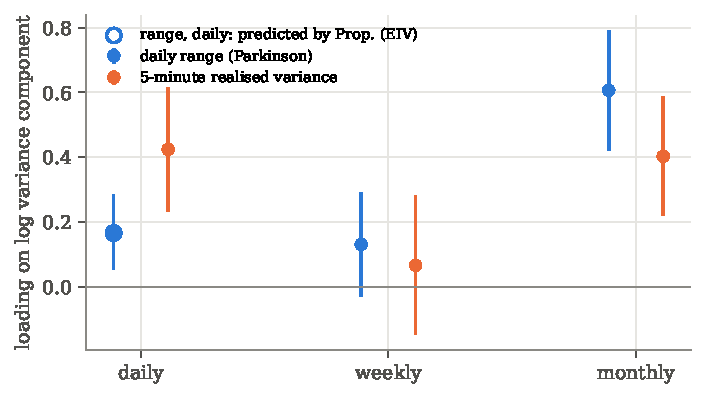
\includegraphics[width=0.78\textwidth]{../results/figures/rv_har_loadings.pdf}
\caption{Log-HAR loadings of the $K=1$ model for CSI~300 with range-based and realised daily variance
(95\% intervals from sandwich standard errors). The hollow circle is the range-based daily loading
predicted by \cref{prop:eiv} from the realised-variance estimate and the measurement-error variances of
\cref{tab:rv-measure}.}\label{fig:rv-har}
\end{figure}

\subsection{Out-of-sample results}

\Cref{tab:rv-oos} reports the walk-forward comparison. Four results stand out.

\emph{Realised measures improve the SMoE everywhere, modestly.} Each of the five realised-variance
specifications has a better log score than SMoE-PK on each of the three series (15 of 15
comparisons). The gains range from $0.14$ to $1.61$ hundredths of a nat per day and are significant
in 4 of the 15 comparisons. They are clearer for the variance forecast itself: on the CSI~300 every
realised specification has a significantly lower QLIKE than SMoE-PK, and against the 5-minute proxy
QLIKE falls from $0.331$ to $0.289$--$0.306$ and the Mincer--Zarnowitz $R^2$ rises from $0.19$ to
$0.34$--$0.36$ (except for SMoE-CJ, whose $R^2$ of $0.11$ illustrates how fragile that statistic is on
variance levels). The refinements of SMoE-RV add little: the overnight term (TV), the jump split
(CJ), the semivariances (SV) and the encompassing model (PKRV) all lie within one hundredth of a nat
of SMoE-RV on every series.

\emph{The mixture still adds to a single regime.} With realised covariates on both sides, SMoE-RV has
a significantly better log score than the single-regime Gauss-HAR-RV on all three series (one-sided
$p\approx0.02$ in each case), and the single-regime models fail the 1\% Kupiec test on more series.
The size of the mixture's advantage shrinks, however, from $0.022$ nats per day with range-based
covariates to $0.016$ with realised ones, a point we return to below.

\emph{A single-regime model with realised variance is the best density forecaster here.} The
log-linear Realized GARCH with Student-$t$ errors has the best log score on all three series. It
beats SMoE-PK significantly everywhere and SMoE-RV significantly on the CSI~300 ($p<0.001$) and the
ETF ($p=0.008$), but not on the IF futures ($p=0.17$). On QLIKE and on the FZ0 tail losses it is
statistically indistinguishable from SMoE-RV, and the 10\% model confidence set for log score keeps
every model except the range-based Gauss-HAR on all three series. We report this result plainly: once a
precise variance measure is available, a GARCH recursion that uses it with fat-tailed errors is
at least as good as three readable regimes, and on two of three series better.

\emph{\Cref{lem:logvar-cost} explains most of the single-regime gains and why the mixture gains less.}
\Cref{tab:rv-lemma} compares the log-score difference predicted from the accuracy of each model's
variance forecast, $\Delta\Var(e_t)/4$, with the difference observed. For the single-regime pair the
prediction is close: $-1.01$ against $-1.15$ hundredths of a nat when the range is replaced by
realised variance; for Realized GARCH it is $-2.43$ against $-2.08$. For the SMoE the observed gains
are roughly a third of the prediction ($-0.49$ against $-1.34$ for SMoE-RV). The lemma assumes a
Gaussian predictive; a scale mixture is less sensitive to an error in its overall variance because
its components already spread probability over several variance levels. Part of the mixture's
advantage in the main results is therefore insurance against a noisy variance covariate, and that
part shrinks when the covariate improves. This is consistent with the smaller mixture advantage
noted above.

\begin{table}[!htbp]\centering\footnotesize
\caption{Realised-variance covariates out of sample (development period)}\label{tab:rv-oos}
\begin{adjustbox}{max width=\textwidth}
\begin{tabular}{lrrrrrrrr}
\toprule
Model & CSI NLL & CSI QLIKE & CSI FZ5 & IF NLL & ETF NLL & QLIKE$_{\mathrm{RV}}$ & MZ $R^2_{\mathrm{RV}}$ & Kupiec 1\%\\
\midrule
SMoE-PK & 1.5727 & 1.5848 & 1.0246 & 1.4866 & 1.4796 & 0.331 & 0.189 & 3\\
SMoE-RV & $-0.49$ & $-2.93^{*}$ & $-1.82$ & $-1.21$ & $-0.97^{*}$ & 0.291 & 0.351 & 3\\
SMoE-TV & $-0.14$ & $-2.42^{*}$ & $-0.72$ & $-0.92$ & $-0.79$ & 0.306 & 0.358 & 3\\
SMoE-CJ & $-0.31$ & $-2.33^{*}$ & $-1.37$ & $-1.50^{*}$ & $-1.08^{*}$ & 0.300 & 0.112 & 3\\
SMoE-SV & $-0.56$ & $-2.12^{*}$ & $-1.70$ & $-1.61^{*}$ & $-0.56$ & 0.289 & 0.338 & 3\\
SMoE-PKRV & $-0.26$ & $-1.79^{*}$ & $-1.00$ & $-0.71$ & $-0.58$ & 0.304 & 0.343 & 3\\
Gauss-HAR-PK & $2.21$ & $-0.67$ & $0.19$ & $0.82$ & $2.43$ & 0.317 & 0.270 & 2\\
Gauss-HAR-RV & $1.06$ & $-3.02^{*}$ & $-1.72$ & $0.17$ & $1.38$ & 0.286 & 0.326 & 1\\
GARCH-t & $-0.51$ & $1.54$ & $1.04$ & $-0.92$ & $-1.02^{*}$ & 0.350 & 0.237 & 3\\
RealGARCH-t & $-2.08^{*}$ & $-3.32^{*}$ & $-1.98$ & $-1.95^{*}$ & $-2.24^{*}$ & 0.272 & 0.401 & 2\\
\bottomrule
\end{tabular}
\end{adjustbox}
\par\smallskip\begin{minipage}{\textwidth}\footnotesize
First row: SMoE-PK losses. Other rows in loss columns: loss of SMoE-PK minus loss of the model, $\times100$ (positive = model better); $^*$: one-sided DM-HLN $p<0.05$ in favour of the model. QLIKE$_{\mathrm{RV}}$ and MZ $R^2_{\mathrm{RV}}$: CSI 300 variance forecasts against $\mathrm{RV}_{t+1}+r^2_{\text{overnight},t+1}$. Kupiec 1\%: series (of 3) on which the 1\% VaR passes at 5\%. Common samples: CSI 300 $n=2850$, IF $n=904$, ETF $n=2062$.
\end{minipage}
\end{table}
\begin{table}[!htbp]\centering\small
\caption{Log-score gains predicted by \cref{lem:logvar-cost} from the accuracy of the variance forecast, CSI 300}\label{tab:rv-lemma}
\begin{adjustbox}{max width=\textwidth}
\begin{tabular}{lrrr}
\toprule
Model & $\Var(e_t)$ & Predicted $\Delta$NLL & Observed $\Delta$NLL\\
\midrule
SMoE-PK & 0.465 & 0.000 & 0.000\\
SMoE-RV & 0.412 & -1.336 & -0.490\\
SMoE-TV & 0.429 & -0.898 & -0.141\\
SMoE-CJ & 0.418 & -1.176 & -0.308\\
SMoE-SV & 0.419 & -1.148 & -0.560\\
SMoE-PKRV & 0.435 & -0.757 & -0.259\\
Gauss-HAR-PK & 0.441 & -0.594 & 2.206\\
Gauss-HAR-RV & 0.401 & -1.604 & 1.055\\
GARCH-t & 0.485 & 0.491 & -0.509\\
RealGARCH-t & 0.368 & -2.428 & -2.083\\
\bottomrule
\end{tabular}
\end{adjustbox}
\par\smallskip\begin{minipage}{\textwidth}\footnotesize
$e_t=\log(\mathrm{RV}_{t+1}+r^2_{\text{overnight},t+1})-\log\hat V_t$, with $\hat V_t$ the forecast variance. Predicted $\Delta$NLL $=\{\Var(e_t)-\Var(e_t^{\text{SMoE-PK}})\}/4$; observed $\Delta$NLL is the out-of-sample log-score difference from SMoE-PK. Both $\times100$, nats per day; negative = better than SMoE-PK. The error of the proxy is common to all models and cancels.
\end{minipage}
\end{table}

\subsection{In-sample white box}

\Cref{tab:rv-insample} re-estimates the CSI~300 SMoE on the days with 5-minute data (June 2009 to
June 2024). Realised covariates raise the log-likelihood by 16.6 (SMoE-RV) and 21.4 (SMoE-TV) points
at the same number of parameters, and BIC selects SMoE-TV. Two of the white-box conclusions of
\cref{sec:results-china} survive the change of variance measure and one weakens. Momentum and drawdown
remain absent from the gate under every specification ($p$ between $0.24$ and $0.45$). The
volatility effect in the gate is weaker on this shorter sample, which starts after the 2007--08
boom and bust: the Wald statistic is $6.5$ ($p=0.04$) with the range, $3.4$ ($p=0.19$) with
trading-session realised variance and $14.6$ ($p<0.001$) when overnight variance is included.
Volatility is still the only candidate regime variable, but how strongly it moves the gate depends on
whether the overnight gap is measured. Finally, the semivariance model does not support the
asymmetry that \citet{patton2015good} find for US stocks: the hypothesis that negative and positive
semivariances have equal loadings in all three experts is not rejected ($W=1.42$, $p=0.70$).

\begin{table}[!htbp]\centering\small
\caption{In-sample fits with range-based and realised variance covariates, CSI 300 (June 2009--June 2024, days with 5-minute data)}\label{tab:rv-insample}
\begin{adjustbox}{max width=\textwidth}
\begin{tabular}{lrrrrr}
\toprule
Model & Log-lik. & Params & BIC & $W$ vol. in gate & $W$ mom.+dd in gate\\
\midrule
SMoE-PK & -5857.5 & 27 & 11,937 & 6.54 (0.038) & 5.53 (0.237)\\
SMoE-RV & -5841.0 & 27 & 11,903 & 3.35 (0.187) & 5.31 (0.257)\\
SMoE-TV & -5836.1 & 27 & 11,894 & 14.56 (0.001) & 3.86 (0.425)\\
SMoE-CJ & -5845.9 & 30 & 11,938 & 1.11 (0.574) & 4.71 (0.318)\\
SMoE-SV & -5839.5 & 30 & 11,925 & 6.46 (0.040) & 3.66 (0.454)\\
SMoE-PKRV & -5829.8 & 36 & 11,955 & 1.33 (0.515) & 4.66 (0.324)\\
Gauss-HAR-PK & -5999.5 & 9 & 12,073 & -- & --\\
Gauss-HAR-RV & -5960.8 & 9 & 11,995 & -- & --\\
\bottomrule
\end{tabular}
\end{adjustbox}
\par\smallskip\begin{minipage}{\textwidth}\footnotesize
Robust Wald statistics ($p$-values) that the volatility state (2 df) and the momentum and drawdown states (4 df) are absent from the gate. Equality of the negative and positive semivariance loadings in all three experts of SMoE-SV: $W=1.42$ (3 df, $p=0.70$).
\end{minipage}
\end{table}

\paragraph{Implications.} The regime structure and the precision of the variance measure are partly
substitutes: a better measure reduces the gain from mixing without removing it. The main results,
which use the range for every series, therefore understate what any model with a precise variance
measure achieves, and they somewhat overstate the share of the SMoE's advantage that is due to its
regimes. Where intraday data exist, the natural next step is an SMoE whose
experts have Realized-GARCH-type variance recursions, which would combine the readable regimes with
the variance dynamics that won here (\cref{sec:agenda}).

\section{Results V: how black are the black boxes?}\label{sec:yardstick}

\subsection{Design}
For each teacher and series we fit, at the start of every calendar year $Y$, an SMoE shadow to ten
draws from the teacher's \emph{out-of-sample} predictive distribution on every earlier date, and use
the shadow to forecast year $Y$. The first three years of each teacher's out-of-sample history serve
as burn-in, so the shadow is evaluated from 2015 onwards on most series. The shadow never sees a
realised return: it learns only what the teacher predicted, and it learns it with information
available at the time. The reference model for the fidelity ratio is the historical Gaussian.
\Cref{tab:yardstick} summarises; \cref{fig:yardstick} shows every series.

\subsection{The deep SMoE is 92\% white}
The deep heterogeneous MoE improves on the historical Gaussian by a median of $0.129$ nats per day.
Its SMoE shadow achieves $0.122$, a median fidelity of $\Phi=0.92$ with interquartile range
$[0.89,0.96]$. The shadow reproduces the deep model's predictive variance almost exactly (median
$R^2$ of log variance $0.88$) but not its predictive mean ($R^2=0.20$), which is consistent with
\cref{sec:results-global}: the deep model's means carry no out-of-sample information, so there is
nothing for a white box to reproduce. The remaining eight percent is not noise: the
Amisano--Giacomini test rejects equal log scores of teacher and shadow on 12 of 19 series, always in
the teacher's favour. The black box knows a little more than three readable regimes do, and the
fidelity ratio measures how much more.

The probes give a complementary reading. The deep model's gate is \emph{not} a function of the
SMoE's state variables: linear probes of its gate logits on volatility, momentum and drawdown have
$R^2$ between $0.04$ and $0.84$ with a median of $0.26$, and only 9 of 57 expert-series probes exceed
$0.5$. The deep network therefore routes observations differently from the SMoE but ends up with
almost the same predictive distribution. When two different internal mechanisms produce the same
input--output map, inspecting internal weights (as the undergraduate thesis did with its gating
plots) can mislead, whereas a yardstick defined on the output cannot.


\subsection{Gradient boosting, Markov switching and GARCH}
The boosted model's shadow reproduces all of its gain ($\Phi=1.03$; log-variance $R^2=0.99$): its
predictive distribution is, to a first approximation, a log-HAR variance with a noisy mean. The
Markov-switching regression has $\Phi=0.93$ with the widest dispersion, reflecting that its latent
regime is filtered from past returns rather than from observables. GARCH-$t$ has $\Phi=0.98$, a useful
sanity check: the SMoE family contains close approximations to the GARCH predictive.

\subsection{Foundation models: the shadow beats the teacher}
The zero-shot Chronos-Bolt forecasts are no better than the historical Gaussian on the median
series (gain $-0.054$ for the small and $-0.004$ for the base model), because their predictive
distributions are too narrow (PIT standard deviations $1.32$ and $1.25$; \cref{sec:results-global}).
Their SMoE shadows, fitted to the same forecasts, gain $+0.035$ and $+0.062$. The small model's shadow
beats its teacher on every series, significantly on 15 of 19; the base model's shadow beats its
teacher on 17 series, significantly on 14. Scaling the foundation model improves its calibration, but
not enough to close the gap to its own white-box reading.

TimesFM~2.5, a different architecture released ten months after Chronos-Bolt, is the first foundation model in
our comparison that beats the historical Gaussian on the median series, by $0.012$ nats per day; its
PIT standard deviation of $1.17$ is the closest to one among the three. The pattern is nevertheless
the same. Its shadow gains $0.043$, beats its teacher on 14 of 19 series and does so significantly on
10, while the teacher is never significantly better than its shadow. Projecting a foundation model
onto a structured likelihood family therefore acts as a regulariser: the shadow keeps the information
in the teacher's location and relative-scale forecasts (median log-variance $R^2$ between $0.48$ and
$0.57$ for the three models) while the semantic variance experts re-anchor the overall scale to the
data. For the Chronos models fidelity is negative because the teacher loses to the reference, and for
TimesFM the teacher's gain is too small for the ratio $\Phi=0.46$ to be read as a share. The common
finding is that none of the three foundation models produces a predictive distribution that is
usable as is, while a white-box reading of each one is.


\begin{figure}[t]\centering
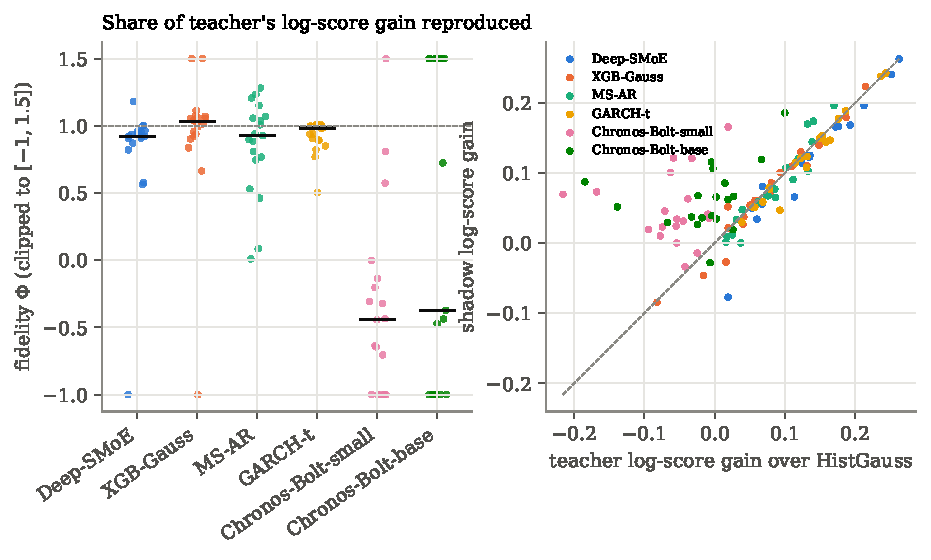
\includegraphics[width=\textwidth]{../results/figures/yardstick.pdf}
\caption{The white-box yardstick. Left: fidelity $\Phi$ per teacher and series (horizontal bars are
medians). Right: out-of-sample log-score gain over the historical Gaussian of each teacher ($x$)
and of its SMoE shadow ($y$); points above the diagonal are series on which the shadow beats its
teacher.}\label{fig:yardstick}
\end{figure}

\begin{table}[!htbp]\centering\scriptsize
\caption{The white-box yardstick: fidelity of SMoE shadows of black-box forecasters (out of sample)}\label{tab:yardstick}
\begin{adjustbox}{max width=\textwidth}
\begin{tabular}{lrrrrrrrr}
\toprule
Teacher & Series & Median LS gain & Median $\Phi$ & $R^2$ mean & $R^2$ log var & $R^2$ P(up) & Median KL & AG reject\\
\midrule
Chronos-Bolt-base & 19 & -0.004 & -0.373 & 0.109 & 0.566 & 0.157 & 0.052 & 14\\
Chronos-Bolt-small & 19 & -0.054 & -0.443 & 0.143 & 0.478 & 0.244 & 0.063 & 15\\
Deep-SMoE & 19 & 0.129 & 0.922 & 0.198 & 0.877 & 0.175 & 0.019 & 12\\
GARCH-t & 19 & 0.131 & 0.983 & 0.003 & 0.804 & 0.249 & 0.016 & 5\\
MS-AR & 19 & 0.086 & 0.927 & 0.282 & 0.579 & 0.379 & 0.025 & 9\\
XGB-Gauss & 19 & 0.060 & 1.032 & 0.013 & 0.986 & 0.035 & 0.007 & 5\\
\bottomrule
\end{tabular}
\end{adjustbox}
\par\smallskip\begin{minipage}{\textwidth}\footnotesize
LS gain: teacher log score minus historical-Gaussian log score. $\Phi$: share of that gain reproduced by the SMoE shadow. AG reject: number of series on which the Amisano--Giacomini test rejects equal log scores of teacher and shadow at 5\%.
\end{minipage}
\end{table}

\section{Results VI: calibration guarantees and economic value}\label{sec:economic}

\subsection{Conformal calibration}\label{sec:conformal-results}
\Cref{tab:conformal} applies the adaptive conformal layer of \cref{thm:aci} with $\eta=0.005$ to the
VaR forecasts of five models on all nineteen series. As the theorem guarantees, after calibration
every model's violation rate is within the bound of the target and the Kupiec test rejects for no
series. The informative comparison is conditional coverage. Calibration fixes the \emph{frequency} of
violations but not their \emph{clustering}: after calibration the historical Gaussian still fails the
Christoffersen conditional-coverage test on 53\% of series at the 5\% level, whereas the calibrated
SMoE fails on none. The conformal layer and the distributional model are complements: the former
delivers the guarantee, the latter makes the violations unpredictable.

\begin{table}[!htbp]\centering\scriptsize
\caption{VaR violations before (raw) and after adaptive conformal calibration (ACI, $\eta=0.005$)}\label{tab:conformal}
\begin{adjustbox}{max width=\textwidth}
\begin{tabular}{lrrrrrr}
\toprule
Model & $a$ & Calibration & Mean rate & Max $|$rate$-a|$ & Kupiec reject & Christoffersen reject\\
\midrule
Deep-SMoE & 0.0100 & ACI & 0.0093 & 0.0029 & 0.0000 & 0.0000\\
Deep-SMoE & 0.0100 & raw & 0.0093 & 0.0074 & 0.2105 & 0.2105\\
Deep-SMoE & 0.0500 & ACI & 0.0483 & 0.0085 & 0.0000 & 0.1053\\
Deep-SMoE & 0.0500 & raw & 0.0423 & 0.0292 & 0.3684 & 0.3158\\
GARCH-t & 0.0100 & ACI & 0.0098 & 0.0012 & 0.0000 & 0.0000\\
GARCH-t & 0.0100 & raw & 0.0125 & 0.0074 & 0.4737 & 0.4211\\
GARCH-t & 0.0500 & ACI & 0.0495 & 0.0046 & 0.0000 & 0.0526\\
GARCH-t & 0.0500 & raw & 0.0543 & 0.0154 & 0.4211 & 0.4737\\
Gauss-HAR & 0.0100 & ACI & 0.0098 & 0.0012 & 0.0000 & 0.0000\\
Gauss-HAR & 0.0100 & raw & 0.0163 & 0.0142 & 0.7895 & 0.8421\\
Gauss-HAR & 0.0500 & ACI & 0.0479 & 0.0069 & 0.0000 & 0.1053\\
Gauss-HAR & 0.0500 & raw & 0.0443 & 0.0312 & 0.3684 & 0.4211\\
HistGauss & 0.0100 & ACI & 0.0101 & 0.0009 & 0.0000 & 0.1579\\
HistGauss & 0.0100 & raw & 0.0203 & 0.0187 & 0.9474 & 1.0000\\
HistGauss & 0.0500 & ACI & 0.0487 & 0.0069 & 0.0000 & 0.5263\\
HistGauss & 0.0500 & raw & 0.0482 & 0.0157 & 0.3684 & 0.7368\\
SMoE & 0.0100 & ACI & 0.0094 & 0.0016 & 0.0000 & 0.0526\\
SMoE & 0.0100 & raw & 0.0096 & 0.0074 & 0.1053 & 0.2632\\
SMoE & 0.0500 & ACI & 0.0485 & 0.0058 & 0.0000 & 0.0000\\
SMoE & 0.0500 & raw & 0.0420 & 0.0253 & 0.5263 & 0.3684\\
\bottomrule
\end{tabular}
\end{adjustbox}
\par\smallskip\begin{minipage}{\textwidth}\footnotesize
Rates averaged over 19 series; reject columns: share of series rejecting at 5\%.
\end{minipage}
\end{table}

\subsection{Trading the CSI 300}
We trade the CSI~300 ETF (long-only, 3bp per side) and IF futures (long/short, 2bp) from the CSI~300
predictive distributions with four rules fixed in advance: the sign of $P(y>0)-1/2$, volatility
targeting at 1\% daily, volatility targeting tilted by $2P(y>0)$, and the mean-variance rule with the
no-trade band of \cref{prop:band} ($\gamma=5$). Decisions are taken at the close and executed at the
next open (\cref{tab:econ_etf510300,tab:econ_if_main}).

Three results summarise the evidence. First, on the ETF several mean-variance rules roughly halve
the maximum drawdown of buy-and-hold (from $-46\%$ to between $-21\%$ and $-27\%$) and raise the
Sharpe ratio from $0.11$ to $0.3$--$0.45$. Second, none of these improvements is statistically
reliable: Sharpe-ratio standard errors are about $0.3$ over twelve years, and every 95\%
stationary-bootstrap interval for the excess return over buy-and-hold contains zero. Third, the
search over models, rules and parameters has to be accounted for. Across the 360 configurations at the
realistic cost level, the deflated Sharpe ratio of the best configuration is $0.76$, below the 0.95
threshold ($0.56$ if all 1,440 configurations across cost levels are counted as trials), and the probability of backtest overfitting is $0.51$ (\cref{tab:overfit}): the
configuration that looks best in one half of the sample is no better than the median configuration in
the other half.

The economic conclusion matches the statistical one. Daily predictive distributions of the CSI~300
are good enough to control risk (exposure falls when regime disagreement and volatility rise, which is
what reduces drawdowns), but they do not deliver reliable directional alpha. The white box shows the
mechanism: positions shrink through the variance term of \eqref{eq:var} rather than through the mean.


\begin{figure}[t]\centering
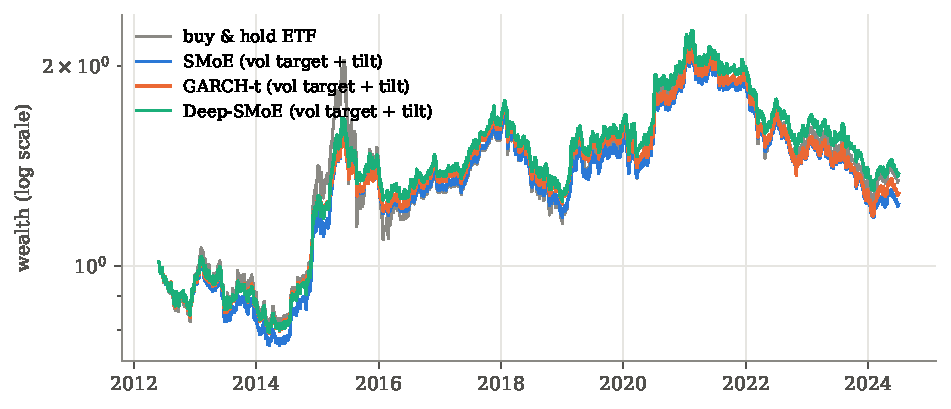
\includegraphics[width=\textwidth]{../results/figures/econ_equity_etf.pdf}
\caption{Wealth of the volatility-target-with-tilt rule on the CSI 300 ETF, net of costs, against
buy and hold.}\label{fig:equity}
\end{figure}

\begin{table}[!htbp]\centering\scriptsize
\caption{Trading results: CSI 300 ETF (510300), long-only, 3bp, out of sample}\label{tab:econ_etf510300}
\begin{adjustbox}{max width=\textwidth}
\begin{tabular}{llrrrrrrrrr}
\toprule
Model & Rule & Return & Vol & Sharpe & SE & MaxDD & Avg $w$ & Turnover & Excess CI lo & Excess CI hi\\
\midrule
Deep-SMoE & meanvar & 0.059 & 0.130 & 0.452 & 0.297 & -0.266 & 0.389 & 41.380 & -0.045 & 0.122\\
Gauss-HAR & meanvar & 0.034 & 0.111 & 0.304 & 0.294 & -0.230 & 0.375 & 14.048 & -0.082 & 0.106\\
SMoE & meanvar & 0.038 & 0.127 & 0.300 & 0.295 & -0.261 & 0.419 & 15.460 & -0.075 & 0.103\\
MAR & meanvar & 0.030 & 0.116 & 0.259 & 0.297 & -0.208 & 0.376 & 6.034 & -0.093 & 0.098\\
Chronos-Bolt-small & meanvar & 0.020 & 0.147 & 0.135 & 0.294 & -0.421 & 0.455 & 20.223 & -0.082 & 0.066\\
HistGauss & meanvar & 0.020 & 0.150 & 0.134 & 0.295 & -0.407 & 0.333 & 0.783 & -0.098 & 0.083\\
GARCH-t & meanvar & 0.016 & 0.156 & 0.102 & 0.293 & -0.476 & 0.806 & 0.845 & -0.065 & 0.052\\
Chronos-Bolt-small & sign & 0.046 & 0.171 & 0.271 & 0.295 & -0.397 & 0.541 & 38.255 & -0.049 & 0.090\\
Deep-SMoE & sign & 0.037 & 0.188 & 0.196 & 0.294 & -0.412 & 0.619 & 68.275 & -0.048 & 0.067\\
HistGauss & sign & 0.030 & 0.179 & 0.171 & 0.295 & -0.438 & 0.486 & 7.033 & -0.070 & 0.083\\
GARCH-t & sign & 0.025 & 0.226 & 0.112 & 0.293 & -0.463 & 1.000 & 0.000 & 0.000 & 0.000\\
MAR & sign & 0.003 & 0.178 & 0.018 & 0.293 & -0.447 & 0.595 & 20.585 & -0.092 & 0.047\\
Gauss-HAR & sign & -0.010 & 0.154 & -0.067 & 0.292 & -0.537 & 0.556 & 50.263 & -0.104 & 0.039\\
SMoE & sign & -0.014 & 0.178 & -0.081 & 0.292 & -0.459 & 0.581 & 29.334 & -0.108 & 0.020\\
HistGauss & voltarget & 0.026 & 0.164 & 0.158 & 0.293 & -0.419 & 0.786 & 0.490 & -0.040 & 0.043\\
GARCH-t & voltarget & 0.021 & 0.150 & 0.141 & 0.293 & -0.441 & 0.795 & 3.262 & -0.051 & 0.047\\
Chronos-Bolt-small & voltarget & 0.023 & 0.181 & 0.128 & 0.293 & -0.461 & 0.912 & 5.697 & -0.037 & 0.037\\
Deep-SMoE & voltarget & 0.018 & 0.151 & 0.118 & 0.293 & -0.434 & 0.803 & 8.872 & -0.057 & 0.042\\
SMoE & voltarget & 0.016 & 0.153 & 0.106 & 0.293 & -0.439 & 0.814 & 7.403 & -0.059 & 0.040\\
Gauss-HAR & voltarget & 0.015 & 0.153 & 0.101 & 0.293 & -0.434 & 0.813 & 9.140 & -0.061 & 0.041\\
MAR & voltarget & 0.015 & 0.152 & 0.098 & 0.293 & -0.433 & 0.810 & 10.543 & -0.062 & 0.041\\
Deep-SMoE & vt\_tilt & 0.027 & 0.158 & 0.173 & 0.293 & -0.425 & 0.813 & 9.437 & -0.038 & 0.046\\
HistGauss & vt\_tilt & 0.027 & 0.167 & 0.159 & 0.294 & -0.422 & 0.786 & 0.688 & -0.037 & 0.041\\
GARCH-t & vt\_tilt & 0.021 & 0.156 & 0.137 & 0.293 & -0.450 & 0.825 & 3.148 & -0.049 & 0.046\\
SMoE & vt\_tilt & 0.018 & 0.157 & 0.117 & 0.293 & -0.443 & 0.819 & 8.233 & -0.050 & 0.040\\
MAR & vt\_tilt & 0.018 & 0.156 & 0.115 & 0.293 & -0.437 & 0.817 & 11.022 & -0.051 & 0.040\\
Gauss-HAR & vt\_tilt & 0.018 & 0.153 & 0.115 & 0.293 & -0.435 & 0.812 & 9.188 & -0.056 & 0.041\\
Chronos-Bolt-small & vt\_tilt & 0.021 & 0.184 & 0.114 & 0.293 & -0.474 & 0.914 & 6.058 & -0.038 & 0.031\\
\bottomrule
\end{tabular}
\end{adjustbox}
\par\smallskip\begin{minipage}{\textwidth}\footnotesize
Buy and hold: Sharpe 0.112, maximum drawdown -0.463. Annualised; decisions at the close, execution at the next open. Excess CI: 95\% stationary-bootstrap interval of the annualised mean return in excess of buy and hold.
\end{minipage}
\end{table}
\begin{table}[!htbp]\centering\scriptsize
\caption{Trading results: IF futures, long/short, 2bp, out of sample}\label{tab:econ_if_main}
\begin{adjustbox}{max width=\textwidth}
\begin{tabular}{llrrrrrrrrr}
\toprule
Model & Rule & Return & Vol & Sharpe & SE & MaxDD & Avg $w$ & Turnover & Excess CI lo & Excess CI hi\\
\midrule
Deep-SMoE & meanvar & 0.067 & 0.156 & 0.430 & 0.376 & -0.261 & 0.094 & 97.980 & -0.089 & 0.203\\
Chronos-Bolt-small & meanvar & 0.045 & 0.170 & 0.267 & 0.372 & -0.269 & 0.092 & 44.951 & -0.099 & 0.200\\
MAR & meanvar & 0.036 & 0.140 & 0.255 & 0.375 & -0.206 & 0.117 & 13.509 & -0.112 & 0.188\\
Gauss-HAR & meanvar & 0.015 & 0.141 & 0.105 & 0.373 & -0.249 & 0.174 & 46.336 & -0.118 & 0.150\\
HistGauss & meanvar & 0.015 & 0.164 & 0.092 & 0.374 & -0.387 & 0.054 & 1.954 & -0.161 & 0.183\\
GARCH-t & meanvar & -0.006 & 0.163 & -0.036 & 0.373 & -0.472 & 0.853 & 1.168 & -0.043 & 0.014\\
SMoE & meanvar & -0.006 & 0.167 & -0.038 & 0.373 & -0.380 & 0.084 & 56.403 & -0.180 & 0.149\\
Chronos-Bolt-small & sign & 0.093 & 0.198 & 0.468 & 0.372 & -0.275 & 0.092 & 78.096 & -0.054 & 0.267\\
Deep-SMoE & sign & 0.084 & 0.199 & 0.420 & 0.374 & -0.273 & 0.243 & 138.900 & -0.060 & 0.223\\
HistGauss & sign & 0.021 & 0.199 & 0.107 & 0.374 & -0.450 & 0.044 & 10.041 & -0.166 & 0.208\\
MAR & sign & 0.019 & 0.196 & 0.098 & 0.374 & -0.430 & 0.199 & 38.490 & -0.146 & 0.177\\
GARCH-t & sign & 0.007 & 0.197 & 0.036 & 0.373 & -0.454 & 1.000 & 0.000 & 0.000 & 0.000\\
SMoE & sign & -0.048 & 0.199 & -0.240 & 0.372 & -0.489 & 0.163 & 64.151 & -0.226 & 0.120\\
Gauss-HAR & sign & -0.068 & 0.197 & -0.344 & 0.373 & -0.521 & 0.155 & 116.029 & -0.238 & 0.084\\
Deep-SMoE & voltarget & 0.002 & 0.157 & 0.015 & 0.373 & -0.428 & 0.853 & 8.430 & -0.031 & 0.021\\
Chronos-Bolt-small & voltarget & 0.003 & 0.184 & 0.014 & 0.373 & -0.460 & 0.952 & 4.643 & -0.017 & 0.008\\
MAR & voltarget & 0.000 & 0.159 & 0.003 & 0.373 & -0.427 & 0.865 & 10.071 & -0.033 & 0.020\\
Gauss-HAR & voltarget & -0.001 & 0.160 & -0.005 & 0.373 & -0.428 & 0.867 & 9.158 & -0.033 & 0.018\\
SMoE & voltarget & -0.001 & 0.161 & -0.009 & 0.373 & -0.432 & 0.870 & 7.578 & -0.034 & 0.016\\
GARCH-t & voltarget & -0.003 & 0.157 & -0.018 & 0.373 & -0.438 & 0.849 & 3.286 & -0.039 & 0.017\\
HistGauss & voltarget & -0.007 & 0.166 & -0.040 & 0.373 & -0.422 & 0.855 & 0.417 & -0.039 & 0.011\\
Deep-SMoE & vt\_tilt & 0.005 & 0.161 & 0.034 & 0.374 & -0.422 & 0.861 & 7.493 & -0.026 & 0.021\\
MAR & vt\_tilt & 0.001 & 0.161 & 0.003 & 0.373 & -0.429 & 0.869 & 10.172 & -0.033 & 0.020\\
Gauss-HAR & vt\_tilt & -0.000 & 0.160 & -0.003 & 0.373 & -0.428 & 0.867 & 9.130 & -0.034 & 0.018\\
Chronos-Bolt-small & vt\_tilt & -0.002 & 0.184 & -0.008 & 0.373 & -0.473 & 0.953 & 4.600 & -0.021 & 0.005\\
GARCH-t & vt\_tilt & -0.002 & 0.162 & -0.015 & 0.373 & -0.448 & 0.874 & 3.094 & -0.036 & 0.015\\
SMoE & vt\_tilt & -0.003 & 0.162 & -0.018 & 0.373 & -0.435 & 0.872 & 8.386 & -0.036 & 0.016\\
HistGauss & vt\_tilt & -0.007 & 0.165 & -0.045 & 0.373 & -0.425 & 0.853 & 0.624 & -0.041 & 0.010\\
\bottomrule
\end{tabular}
\end{adjustbox}
\par\smallskip\begin{minipage}{\textwidth}\footnotesize
Buy and hold: Sharpe 0.036, maximum drawdown -0.454. Annualised; decisions at the close, execution at the next open. Excess CI: 95\% stationary-bootstrap interval of the annualised mean return in excess of buy and hold.
\end{minipage}
\end{table}
\begin{table}[!htbp]\centering\small
\caption{Backtest overfitting diagnostics}\label{tab:overfit}
\begin{adjustbox}{max width=\textwidth}
\begin{tabular}{rp{3.5cm}rrp{3.5cm}rrr}
\toprule
Trials & Best (all costs) & Sharpe (all) & DSR (all) & Best at 3bp & Sharpe (3bp) & DSR (3bp) & PBO (3bp)\\
\midrule
1,440 & Deep-SMoE, meanvar, c0.0, g10.0, v0.8 & 0.583 & 0.565 & Gauss-HAR, meanvar, c3.0, g10.0, v0.8 & 0.498 & 0.758 & 0.514\\
\bottomrule
\end{tabular}
\end{adjustbox}
\par\smallskip\begin{minipage}{\textwidth}\footnotesize
DSR: deflated Sharpe ratio, the probability that the true Sharpe ratio exceeds the expected maximum of the trials under the null; values below 0.95 are not significant. PBO: probability of backtest overfitting by combinatorially symmetric cross-validation with 16 blocks.
\end{minipage}
\end{table}

\section{Results VII: the lockbox}\label{sec:lockbox}

All modelling choices (covariates, number of experts, penalties, refit schedules, trading rules and
their parameters) were fixed on the development sample ending 30 June 2024. We then re-estimated every
model from scratch on data up to 30 June 2024 and ran the same walk-forward through 28 October 2026,
a period of 563 to 849 trading days per series that includes the September 2024 policy rally in China
and the April 2025 tariff shock. The lockbox was evaluated once; no result in
this section fed back into any choice.

\paragraph{Density forecasts.} The ranking of model families survives intact (\cref{tab:lockbox}). The
four mixture models occupy the top four average ranks on log score (LSTAR $3.05$, SMoE $3.11$, MAR
$3.21$, deep SMoE $3.26$), and the SMoE has the best average rank on QLIKE ($2.95$) and on the FZ0 tail
loss ($3.16$). The SMoE is in the 10\% model confidence set for every one of the nineteen series under
all four losses. Pairwise, it is better than GARCH-$t$ on 14 series (significantly on 3, significantly
worse on none), and significantly better than the Markov-switching regression on 12, the Gauss-HAR on
9, the boosted model on 7 and both foundation models on 18 series. Against the other mixtures (MAR,
deep SMoE) the lockbox is too short to separate the models: each comparison produces one significant
win and one significant loss.

\paragraph{Calibration.} The SMoE's 1\% VaR passes the Kupiec test on 18 of 19 series (GARCH-$t$: 18;
Chronos-Bolt: 1). Its PIT standard deviation is $1.01$, whereas the foundation models' remain at
$1.31$--$1.35$. After adaptive conformal calibration no model fails the Kupiec test on any series, and
the SMoE and deep SMoE pass the conditional-coverage test on every series at the 5\% level.

\paragraph{Realised variance.} The 5-minute data cover only the first 246 lockbox days. On QLIKE against
realised variance the mixtures again lead (MAR $0.567$, LSTAR $0.598$, SMoE $0.606$, GARCH-$t$ $0.663$).
The Mincer--Zarnowitz $R^2$, however, is highest for the two foundation models ($0.55$ and $0.71$ against
at most $0.13$ for the others). The $R^2$ of a regression on 246 days is dominated by the realised
variance spike of late September 2024, and the zero-shot models, which condition on the raw return path,
scaled up faster after the first large moves. We report this as the one lockbox result in which a
foundation model leads; on the robust loss it does not.

\paragraph{Trading.} The strategies do not beat buy and hold in the lockbox. On the ETF, the best
configuration at 3bp is a GARCH-$t$ mean-variance rule with Sharpe ratio $0.74$ against $0.38$ for buy
and hold, but its standard error is $0.65$, its deflated Sharpe ratio $0.65$ and the probability of
backtest overfitting across the 360 configurations rises to $0.77$ (\cref{tab:overfit_lockbox}). The
SMoE-based volatility-target rules match the buy-and-hold Sharpe ratio ($0.37$ versus $0.38$) with a
smaller maximum drawdown ($-17\%$ versus $-19\%$). The lockbox thus confirms the development-period
conclusion: the predictive distributions manage risk, and the data do not support claims of timing
alpha.

\begin{table}[!htbp]\centering\scriptsize
\caption{Development period versus lockbox: average ranks across 19 series (1 = best), model-confidence-set membership (10\%) and Kupiec passes}\label{tab:lockbox}
\begin{adjustbox}{max width=\textwidth}
\begin{tabular}{llrrrrrrrr}
\toprule
Period & Model & Rank NLL & Rank CRPS & Rank QLIKE & Rank FZ5 & MCS NLL & MCS QLIKE & MCS FZ5 & Kupiec 1\% pass\\
\midrule
Development 2012--2024/06 & SMoE & 2.95 & 3.63 & 3.47 & 4.26 & 15 & 18 & 18 & 17\\
Development 2012--2024/06 & Deep-SMoE & 3.26 & 5.26 & 3.53 & 3.63 & 14 & 17 & 18 & 15\\
Development 2012--2024/06 & MAR & 3.47 & 3.42 & 3.58 & 3.95 & 15 & 18 & 18 & 16\\
Development 2012--2024/06 & LSTAR & 4.00 & 5.00 & 4.05 & 4.00 & 11 & 17 & 18 & 15\\
Development 2012--2024/06 & GARCH-t & 4.11 & 5.26 & 5.95 & 5.16 & 11 & 11 & 15 & 10\\
Development 2012--2024/06 & AR-GJR-t & 3.63 & 3.68 & 5.47 & 4.11 & 17 & 15 & 18 & 12\\
Development 2012--2024/06 & Gauss-HAR & 7.58 & 8.16 & 4.84 & 5.16 & 2 & 16 & 15 & 4\\
Development 2012--2024/06 & MS-AR & 7.89 & 9.89 & 8.00 & 7.42 & 1 & 6 & 11 & 16\\
Development 2012--2024/06 & XGB-Gauss & 8.47 & 4.63 & 7.00 & 8.26 & 1 & 10 & 9 & 2\\
Development 2012--2024/06 & Chronos-Bolt-base & 10.47 & 7.95 & 10.26 & 10.63 & 0 & 2 & 2 & 0\\
Development 2012--2024/06 & HistGauss & 10.26 & 11.47 & 10.00 & 9.68 & 1 & 6 & 7 & 1\\
Lockbox 2024/07--2026/10 & SMoE & 3.11 & 3.42 & 2.95 & 3.16 & 19 & 19 & 19 & 18\\
Lockbox 2024/07--2026/10 & Deep-SMoE & 3.26 & 3.53 & 3.89 & 3.74 & 19 & 19 & 19 & 17\\
Lockbox 2024/07--2026/10 & MAR & 3.21 & 3.11 & 3.16 & 3.58 & 19 & 19 & 19 & 18\\
Lockbox 2024/07--2026/10 & LSTAR & 3.05 & 3.32 & 3.63 & 3.68 & 19 & 19 & 19 & 18\\
Lockbox 2024/07--2026/10 & GARCH-t & 4.37 & 6.21 & 6.63 & 6.11 & 18 & 19 & 18 & 18\\
Lockbox 2024/07--2026/10 & AR-GJR-t & 5.05 & 6.16 & 6.95 & 6.11 & 18 & 19 & 18 & 17\\
Lockbox 2024/07--2026/10 & Gauss-HAR & 7.58 & 6.68 & 4.26 & 4.68 & 15 & 19 & 19 & 14\\
Lockbox 2024/07--2026/10 & MS-AR & 7.16 & 9.05 & 7.79 & 7.84 & 18 & 18 & 18 & 15\\
Lockbox 2024/07--2026/10 & XGB-Gauss & 8.32 & 4.95 & 6.37 & 6.26 & 17 & 19 & 19 & 6\\
Lockbox 2024/07--2026/10 & Chronos-Bolt-base & 10.74 & 9.58 & 10.63 & 11.05 & 4 & 8 & 9 & 1\\
Lockbox 2024/07--2026/10 & HistGauss & 10.47 & 11.32 & 10.05 & 10.05 & 12 & 18 & 16 & 8\\
\bottomrule
\end{tabular}
\end{adjustbox}
\par\smallskip\begin{minipage}{\textwidth}\footnotesize
Ranks among the twelve forecasters (Chronos-Bolt-small not shown). MCS and Kupiec columns count series out of 19.
\end{minipage}
\end{table}
\begin{table}[!htbp]\centering\small
\caption{Lockbox: backtest overfitting diagnostics (CSI 300 ETF, 360 configurations at 3bp)}\label{tab:overfit_lockbox}
\begin{adjustbox}{max width=\textwidth}
\begin{tabular}{p{6cm}rrr}
\toprule
Best at 3bp & Sharpe & DSR & PBO\\
\midrule
GARCH-t, meanvar, c3.0, g5.0, v0.8 & 0.738 & 0.648 & 0.770\\
\bottomrule
\end{tabular}
\end{adjustbox}
\end{table}

\subsection{Do foundation models remember the test period?}\label{sec:fm-release}

A zero-shot forecaster is out of sample only if its pretraining corpus ends before the forecast
date. The documented corpora of Chronos and TimesFM~2.5 do not list the series we study, but
they cannot be audited series by series, and \citet{sarkar2024lookahead} and
\citet{glasserman2024assessing} show that look-ahead through pretraining is real for language
models used in finance. A model's release date $C$ bounds its data cut-off from above, which gives a
simple test.

\begin{proposition}[Release-date test]\label{prop:release}
Let $d_t=\mathrm{NLL}^{\mathrm{FM}}_t-\mathrm{NLL}^{\mathrm{ref}}_t$ be the log-score loss of a
foundation model relative to a reference model estimated in real time, averaged across series on date
$t$, and let $d^{\mathrm{pl}}_t$ be the same difference for a placebo model that is also estimated in
real time. Suppose that, without pretraining overlap, $\E[d_t-d^{\mathrm{pl}}_t]$ is the same before
and after $C$ (parallel trends). Then the coefficient $b$ in
$d_t-d^{\mathrm{pl}}_t=a+b\,\1\{t\ge C\}+e_t$ is zero, and its Newey--West $t$-statistic is
asymptotically standard normal as the numbers of pre- and post-release dates grow. If the corpus
contains the evaluation series up to some cut-off $C'\le C$, forecasts before $C'$ are partly
in-sample and $b>0$. If $C'<C$, dates in $[C',C)$ are classified as pre-release although they are
unseen, which biases $b$ towards zero; the test remains valid but loses power.
\end{proposition}

\noindent The proof is the usual argument for a difference in means with a HAC variance; the content
is in the identifying assumption. Shifts in market conditions at $C$ that change how all models
perform relative to the SMoE are removed by the placebo, for which we use GARCH-$t$. We apply the test
with the release dates of Chronos-Bolt (26 November 2024) and TimesFM~2.5 (15 September 2025), using
the development and lockbox forecasts together.

%RESULTS-RELEASE%

\section{A research agenda}\label{sec:agenda}

The SMoE is minimal by design. Each extension below keeps the white-box property (closed-form
predictive functionals, exact attribution and likelihood-based inference) and each is a
self-contained research question.

\paragraph{1. Multivariate SMoE for allocation.}
Replace the univariate experts by $\N_d(\bm B_k\tilde\bx,\bm\Sigma_k(\bv))$ with regime-specific
covariance matrices, e.g.\ $\bm\Sigma_k=\bm D_k\bm R_k\bm D_k$ with log-linear $\bm D_k$. The
predictive covariance decomposes as $\sum_k\pi_k\bm\Sigma_k+\sum_k\pi_k(\bm\mu_k-\bar{\bm\mu})(\bm\mu_k-\bar{\bm\mu})^\top$,
and the second term is a rank-$(K-1)$ ``regime-disagreement'' factor structure. Open questions:
identification with many assets, shrinkage of $\bm R_k$, and whether regime-disagreement factors are
priced.

\paragraph{2. Decision-focused estimation.}
\Cref{sec:lagging} traces the lagging paradox to a mismatch between the training loss and the use of the
forecast. A natural next step estimates $\btheta$ by maximising realised utility,
$\max_{\btheta}\sum_tU(w_t(\btheta)y_t)$ with $w_t$ given by \cref{prop:band}, or a convex combination of
utility and likelihood. The questions are statistical (consistency of a non-likelihood M-estimator
whose criterion is non-smooth because of the no-trade band) and economic (does it beat
predict-then-optimise out of sample?).

\paragraph{3. Language-model gates.}
Gate covariates need not be prices. Policy statements, regulatory announcements and news can be
mapped by a large language model to a small set of scores (e.g.\ policy stance, liquidity support,
risk-off intensity) that enter $\bz_t$. The SMoE then answers a sharp question (does text move
regime probabilities beyond what prices already imply?) with the score test of \cref{prop:lm-gate},
which needs only the price-based fit and can screen many text scores at once, followed by a Wald test
on the selected $\bm\gamma$ coefficients. The fidelity ratio then measures how much of an LLM-based
black-box forecaster the text-augmented SMoE explains. Because language models also carry look-ahead
in their pretraining, the scores should come from models with dated corpora (item 8).

\paragraph{4. Online Bayesian SMoE.}
Quarterly re-estimation is a crude response to non-stationarity. Sequential Monte Carlo or online
variational EM would update $\btheta$ daily with forgetting, give posterior uncertainty about the
regime parameters themselves, and allow the gate to reflect parameter uncertainty in the predictive
distribution. The adaptive conformal layer of \cref{thm:aci} would then calibrate a Bayesian rather
than a frequentist predictive.

\paragraph{5. Intraday SMoE.}
With 5-minute data the same model can forecast intraday returns and realised variance, with experts
for opening auction, lunch break and closing auction dynamics specific to the Chinese market, and gates
driven by order-flow imbalance. Microstructure noise makes the distributional target essential.

\paragraph{6. Realised-variance experts.}
\Cref{sec:rv} found that a single-regime Realized GARCH beats every SMoE variant in log score once
5-minute data are available, and that part of the mixture's advantage with range-based covariates is
insurance against a noisy variance measure. The obvious synthesis gives each expert its own
measurement equation and variance recursion,
$\log\sigma^2_{kt}=\omega_k+\beta_k\log\sigma^2_{k,t-1}+\gamma_k\log\mathrm{RV}_{t-1}$, with the
gate deciding which recursion governs tomorrow. The CM-step for the variance block is then no longer
a static Gamma regression but a filtering problem, and identification of regime-specific persistence
from a single realised series is open. Extending realised measures to the other eighteen series
requires intraday data we do not have.

\paragraph{7. Yardstick for foundation models.}
As time-series foundation models grow, the fidelity ratio becomes a general tool: for each model and
asset it reports how much of the model's out-of-sample density-forecast gain is reproducible by a
three-regime, ten-covariate white box. A benchmark of $\Phi$ across model families, horizons and
asset classes would make ``how black is the black box?'' a measurable property. Newer models with
covariate and multivariate inputs, such as TimesFM~3.0, can be given the SMoE's own covariates, which
turns the yardstick into a direct comparison of what the network and the white box do with the same
information.

\paragraph{8. Point-in-time foundation models.}
The release-date test of \cref{sec:lockbox} can only bound pretraining look-ahead from one side,
because a model's release date is an upper bound on its data cut-off. Foundation models pretrained on
corpora that end at known, staggered dates would turn the test into an exact event study: the same
architecture trained to vintages $C_1<C_2<\dots$ and evaluated on the same returns identifies how much
of an apparent forecasting gain is memory. \citet{sarkar2024lookahead} make the same argument for
language models.


\section{Conclusion}\label{sec:conclusion}

This paper started from the question whether a heterogeneous mixture-of-experts network can forecast
the CSI~300. Under a leak-free protocol no model in our comparison forecasts daily means or directions,
and the accuracy figures that motivated the original work came from look-ahead. We therefore asked
what a forecaster knows about the conditional distribution of returns and whether that knowledge can
be written down. The Semantic Mixture of Experts answers this for itself in closed form with standard
errors, and for other forecasters through the KL projection.

Four findings carry over beyond this paper. First, price-level losses cannot reveal skill, and the
differenced directional-accuracy metric measures sign persistence in the data rather than anything
about the model (\cref{prop:bound,prop:da}). Second, a three-regime white box with ten covariates matches the density forecasts of a
deep heterogeneous MoE to within eight percent of its gain and dominates single-regime, Markov
switching, boosted and zero-shot foundation models; most of the value comes from variance dynamics
and mixture shape, and the gate's state dependence adds a smaller, testable increment. Third, the
white box produces economic content that a black box hides: in the CSI~300, volatility alone moves
regime weights, and the short-horizon regime continues in China but reverses in developed markets.
Fourth, risk forecasts are where distributional models pay off (tail calibration, a conformal coverage
guarantee and lower drawdowns) whereas claims of directional alpha should be met with deflated Sharpe
ratios and backtest-overfitting probabilities before anyone acts on them.

The limitations are those of a first step. The model is univariate and daily; its gate uses three
hand-chosen state variables; the foundation models enter zero-shot and through a Gaussian projection
of their quantiles; and our economic analysis concerns one market and two instruments. The research
agenda of \cref{sec:agenda} lists the extensions we consider most promising (multivariate and
decision-focused SMoEs, language-model gates and online Bayesian updating). Each keeps the property
that made this exercise informative: every statement the model makes comes with a closed form and a
standard error that a reader can check.


\bibliographystyle{apalike}
\bibliography{refs}

\appendix
\section{Proofs}\label{app:proofs}

\paragraph{Proof of \cref{prop:optimal-level}.}
Conditional on $\F_t$, $P_{t+1}=P_te^{r_{t+1}}$ and $P_t$ is known. For any $\F_t$-measurable $f$,
$\E[(P_{t+1}-f)^2\mid\F_t]=\Var(P_{t+1}\mid\F_t)+(\E[P_{t+1}\mid\F_t]-f)^2$, minimised at
$f^\ast=\E[P_{t+1}\mid\F_t]=P_tM_t(1)$ with value
$\Var(P_{t+1}\mid\F_t)=P_t^2\{M_t(2)-M_t(1)^2\}$. For $f=P_t$ the value is
$P_t^2\E[(e^{r}-1)^2\mid\F_t]=P_t^2\{M_t(2)-2M_t(1)+1\}$; subtracting gives \eqref{eq:mse-gap}.\qed

\paragraph{Proof of \cref{prop:bound}.}
Divide \eqref{eq:mse-gap} by the random-walk MSE: the ratio is
$\rho_t=(M_1-1)^2/(M_2-2M_1+1)$. Under normality $M_1=e^{m}$ and $M_2=e^{2m+\sigma^2}$ with
$m=\mu+\sigma^2/2$. Expanding, $M_1-1=m+O(m^2)$ and
$M_2-2M_1+1=e^{2m}(e^{\sigma^2}-1)+(e^{m}-1)^2=\sigma^2+m^2+O(\sigma^3)$ since $m=O(\sigma)$ for
bounded $s$. Hence $\rho_t=m^2/(\sigma^2+m^2)+O(\sigma^3)=s_t^2/(1+s_t^2)+O(\sigma^3)$. For the
unconditional statement write the optimal and RW MSEs as $\E[P_t^2\{\cdot\}]$; the ratio of
expectations is the $w_t$-weighted average of $\rho_t$ with $w_t\propto P_t^2(\sigma_t^2+m_t^2)$,
and $\mathrm{RMSE}$ ratios are square roots of MSE ratios. The approximation uses
$\sqrt{1-x}\approx1-x/2$.\qed

\paragraph{Proof of \cref{prop:da}.}
If $f_{t+1}=P_t$ then $f_{t+1}-f_t=P_t-P_{t-1}$, whose sign equals that of $r_t$, while
$P_{t+1}-P_t$ has the sign of $r_{t+1}$. The expectation follows from
$\1\{\operatorname{sign}a=\operatorname{sign}b\}=\tfrac12(1+\operatorname{sign}a\operatorname{sign}b)$ for non-zero $a,b$. If
$f_{t+1}=P_t+\varepsilon_{t+1}$ then $f_{t+1}-f_t=(P_t-P_{t-1})+(\varepsilon_{t+1}-\varepsilon_t)$,
which has the sign of $r_t$ whenever $|\varepsilon_{t+1}-\varepsilon_t|<|P_t-P_{t-1}|$; the stated
condition is the same inequality in log units to first order.\qed

\paragraph{Proof of \cref{prop:ident}.}
Fix covariates $(\bx,\bv,\bz)$ in the open set of \cref{ass:ident}(a). Finite mixtures of
univariate normals are identifiable \citep{teicher1963identifiability}: equality of the mixtures
implies equality of the sets $\{(\pi_k,\mu_k,\sigma_k^2)\}_{k}$ and $\{(\pi'_k,\mu'_k,\sigma'^2_k)\}_k$,
which by \cref{ass:ident}(b) have $K$ distinct elements on a set of positive probability. Hence there
is a permutation $\varsigma_{(\bx,\bv,\bz)}$ with
$(\pi'_{\varsigma(k)},\mu'_{\varsigma(k)},\sigma'^2_{\varsigma(k)})=(\pi_k,\mu_k,\sigma_k^2)$. All
component parameters are continuous in the covariates and distinct, so $\varsigma$ is locally
constant and therefore constant on the connected open set. Suppose $\varsigma(k)=l\neq k$. Then
$\bm\beta_k^\top\tilde\bx^{(k)}=\bm\beta_l'^\top\tilde\bx^{(l)}$ on an open set. By
\cref{ass:ident}(c) the two covariate sets differ, so one side varies with a covariate on which the
other does not depend; non-singularity of the designs forces the corresponding slope to be zero,
contradicting (c), unless both experts have no slopes, which (c) excludes for more than one expert.
Hence $\varsigma$ is the identity. Equality of $\mu_k$, $\log\sigma_k^2$ and of the log-odds
$\log(\pi_k/\pi_K)=\bm\gamma_k^\top\tilde\bz$ as linear functions on an open set, together with
non-singular designs, gives $\bm\beta_k=\bm\beta'_k$, $\bm\delta_k=\bm\delta'_k$ and
$\bm\gamma_k=\bm\gamma'_k$.\qed

\paragraph{Proof of \cref{prop:ergodic}.}
Write $Y_t=(y_t,\dots,y_{t-p+1})$. The chain is a $\varphi$-irreducible, aperiodic $T$-chain because
the transition density is a positive Gaussian mixture, and compact sets are small
\citep[Ch.~5--6]{meyn2009markov}. Let $\rho=\sup_{\bz}\sum_k\pi_k(\bz)\sum_j|\phi_{kj}|<1$ and choose
$V(Y)=1+\sum_{j=1}^pc_j|y_{t-j+1}|$ with $c_1=1$ and $c_j$ decreasing geometrically so that
$c_{j+1}+\rho_j\le c_j\rho'$ for some $\rho<\rho'<1$, where $\rho_j=\sup_{\bz}\sum_k\pi_k|\phi_{kj}|$.
Then
$\E[|y_{t+1}|\mid Y_t]\le\sum_k\pi_k(|\phi_{k0}|+\sum_j|\phi_{kj}||y_{t-j+1}|)+\bar\sigma\sqrt{2/\pi}$,
so $\E[V(Y_{t+1})\mid Y_t]\le\rho'V(Y_t)+C$ for a constant $C$. The Foster--Lyapunov criterion
\citep[Thm.~15.0.1]{meyn2009markov} yields geometric ergodicity with
$\E_{\text{stat}}V<\infty$.\qed

\paragraph{Proof of \cref{prop:closed}.}
Mean, cdf and probability statements are linear in the mixture weights. The variance follows from
the law of total variance with the component label as conditioning variable. For ES, write
$\E[y\1\{y\le q\}]=\sum_k\pi_k\E[y\1\{y\le q\}\mid k]$ and use
$\E[X\1\{X\le q\}]=\mu\Phi(z)-\sigma\varphi(z)$ for $X\sim\N(\mu,\sigma^2)$, $z=(q-\mu)/\sigma$.
For CRPS use $\mathrm{CRPS}(F,y)=\E|X-y|-\tfrac12\E|X-X'|$ with $X,X'\stackrel{iid}{\sim}F$, and
$\E|Z|=A(m,s^2)$ for $Z\sim\N(m,s^2)$ \citep{grimit2006continuous}. Uniqueness of $q_\alpha$ holds
because the mixture cdf is continuous and strictly increasing.\qed

\paragraph{Proof of \cref{prop:monotone}.}
For any $\btheta$, Jensen's inequality gives
$\ell^\lambda_n(\btheta)-\ell^\lambda_n(\btheta^{(s)})\ge Q(\btheta\mid\btheta^{(s)})-Q(\btheta^{(s)}\mid\btheta^{(s)})$
\citep{dempster1977maximum}. Each CM step does not decrease $Q$: CM-step 1 maximises a strictly
concave quadratic exactly; CM-steps 2 and 3 take Newton steps on strictly concave objectives with step
halving that accepts only non-decreasing values. Hence $Q(\btheta^{(s+1)}\mid\btheta^{(s)})\ge
Q(\btheta^{(s)}\mid\btheta^{(s)})$ and the claim follows; the final L-BFGS step is accepted only if it
increases $\ell^\lambda_n$. Convergence of limit points to stationary points follows from
\citet[Thm.~1]{wu1983convergence} applied to the generalised EM map.\qed

\paragraph{Proof of \cref{prop:elasticity}.}
For the softmax with $\bm\gamma_K=\bm0$,
$\partial\pi_k/\partial z_j=\pi_k(\gamma_{kj}-\sum_l\pi_l\gamma_{lj})$. Since $z_j$ enters neither
$\mu_k$ nor $\sigma_k$, $\partial\bar\mu/\partial z_j=\sum_k\mu_k\partial\pi_k/\partial z_j$ and
$\partial P(y>0)/\partial z_j=\sum_k\Phi(\mu_k/\sigma_k)\partial\pi_k/\partial z_j$.\qed

\paragraph{Proof of \cref{prop:fidelity}.}
$\E\log p(y_t\mid\cdot)=\E\int p_0\log p=\E\int p_0\log p_0-\E\int p_0\log(p_0/p)=-H(p_0)-\E\KL(p_0\|p)$.
The entropy cancels in differences.\qed

\paragraph{Proof of \cref{thm:aci}.}
Summing \eqref{eq:aci} gives $\alpha_{T+1}=\alpha_1+\eta\sum_{t=1}^T(a-\mathrm{err}_t)$. If
$\alpha_t\le0$ then $q_t=-\infty$, $\mathrm{err}_t=0$ and $\alpha_{t+1}=\alpha_t+\eta a>\alpha_t$; if
$\alpha_t\ge1$ then $\mathrm{err}_t=1$ and $\alpha_{t+1}<\alpha_t$. Each step moves $\alpha$ by at
most $\eta$, so $\alpha_t\in[-\eta,1+\eta]$ for all $t$ when $\alpha_1\in(0,1)$. Therefore
$|\sum_t(a-\mathrm{err}_t)|=|\alpha_{T+1}-\alpha_1|/\eta\le(\max(\alpha_1,1-\alpha_1)+\eta)/\eta$,
and dividing by $T$ gives the bound \citep[cf.][Prop.~4.1]{gibbs2021adaptive}.\qed

\paragraph{Student-$t$ densities as Gaussian mixtures.}
All benchmarks are scored through the closed forms of \cref{prop:closed}, which requires a Gaussian
mixture representation. For the Student-$t$ benchmarks we use the scale-mixture identity
$t_\nu(\mu,s)=\int_0^\infty\N(\mu,s^2/\lambda)\,g(\lambda)\,d\lambda$ with
$\lambda\sim\mathrm{Gamma}(\nu/2,\text{rate }\nu/2)$. Substituting $u=\nu\lambda/2$,
\begin{equation}
  \E[h(\lambda)]=\frac{1}{\Gamma(\nu/2)}\int_0^\infty h(2u/\nu)\,u^{\nu/2-1}e^{-u}\,du
  \approx\sum_{i=1}^{N}\omega_i\,h(2u_i/\nu),
\end{equation}
where $(u_i,\tilde\omega_i)$ are the nodes and weights of $N$-point generalised Gauss--Laguerre
quadrature with parameter $\alpha=\nu/2-1$ and $\omega_i=\tilde\omega_i/\Gamma(\nu/2)$. The rule is
exact for polynomials of degree $2N-1$ in $u$; for the smooth integrands $h(\lambda)=\varphi(y;\mu,s^2/\lambda)$
the error decays in $N$ at fixed $y$, more slowly for heavier tails. We use $N=64$. The maximal
relative density error on $|y-\mu|\le4s$ is $0.27\%$ for $\nu=2.5$, $0.11\%$ for $\nu=3$, $0.02\%$
for $\nu=4$ and below $0.005\%$ for $\nu\ge5$ (computed against the exact $t$ density in the
replication package), an order of magnitude below the log-score differences we interpret. An
earlier version with $N=16$ had errors of up to $2.9\%$ at $\nu=3$; we report this because the choice
of $N$ matters for heavy-tailed benchmarks.\qed

\paragraph{Proof of \cref{prop:shrink}.}
By \eqref{eq:var}, $V_t=W_t+B_t=W_t(1+B_t/W_t)$, so $w^\ast_t=\bar\mu_t/(\gamma V_t)$ factorises as
stated. $B_t\ge0$ with equality iff $\mu_{kt}=\bar\mu_t$ for all $k$ with $\pi_{kt}>0$; a
mean-preserving spread of $(\mu_{kt})$ increases $B_t$ and leaves $\bar\mu_t$ and $W_t$ unchanged.\qed

\paragraph{Proof of \cref{prop:band}.}
The objective $J(w)=w\bar\mu-\tfrac\gamma2w^2V-\kappa|w-w_-|$ is strictly concave. Its
superdifferential is $\bar\mu-\gamma Vw-\kappa\,\partial|w-w_-|$. If $|w_--w^\ast|\le b$ then $0$
lies in the superdifferential at $w=w_-$ (take the subgradient $(\bar\mu-\gamma Vw_-)/\kappa\in[-1,1]$).
If $w_-<w^\ast-b$ the optimum is at $w>w_-$ where the first-order condition
$\bar\mu-\gamma Vw-\kappa=0$ gives $w=w^\ast-b$; symmetrically for $w_->w^\ast+b$. Concavity makes
projection onto the box optimal for the constrained problem.\qed

\paragraph{Proof of \cref{prop:ident-shared}.}
The first part of the proof of \cref{prop:ident} does not use \cref{ass:ident}(c): it yields a
permutation $\varsigma$, constant on a connected open set of covariates, with
$(\pi'_{\varsigma(k)},\mu'_{\varsigma(k)},\sigma'^2_{\varsigma(k)})=(\pi_k,\mu_k,\sigma_k^2)$. For a pair of
experts with different covariate sets the argument of \cref{prop:ident} still excludes
$\varsigma(k)=l$. Hence $\varsigma$ can only permute experts within a shared group. Suppose it
exchanges $k$ and $l$ with $\delta_{k,0}<\delta_{l,0}$. Equality of the log variances as linear
functions of $\tilde\bv$ on an open set gives $\bm\delta'_l=\bm\delta_k$ and $\bm\delta'_k=\bm\delta_l$,
so $\delta'_{k,0}=\delta_{l,0}>\delta_{k,0}=\delta'_{l,0}$, which violates the convention for
$\btheta'$. Thus $\varsigma$ is the identity and the remainder of the proof of \cref{prop:ident}
applies. The convention requires $\delta_{k,0}\neq\delta_{l,0}$; if the two variance functions
coincided, an ordering of the mean intercepts would serve the same purpose.\qed

\paragraph{Proof of \cref{prop:lm-gate}.}
The score expression \eqref{eq:lm-score} is \eqref{eq:score} for the gate block with $\tilde\bz_t$
replaced by the augmented vector, evaluated at $\bm\psi=\bm0$, where the prior probabilities
$\pi_{tk}$ do not depend on $\bm w_t$. Write $\bm\vartheta=(\btheta,\bm\psi)$,
$\bm s_n(\bm\vartheta)=\sum_t\partial\ell_t(\bm\vartheta)$ and $A$ for the information matrix (minus the
expected Hessian) of the augmented model at $\bm\vartheta^\ast=(\btheta^\ast,\bm0)$. Under $H_0$,
$\bm\vartheta^\ast$ is the pseudo-true value, so $\E\,\partial\ell_t(\bm\vartheta^\ast)=\bm0$ and, by the
central limit theorem for $\beta$-mixing sequences under \cref{ass:asym},
$n^{-1/2}\bm s_n(\bm\vartheta^\ast)\xrightarrow{d}\N(\bm0,B)$. The restricted estimator satisfies
$\sqrt n(\hat\btheta-\btheta^\ast)=A_{\theta\theta}^{-1}n^{-1/2}\bm s_{n,\theta}(\bm\vartheta^\ast)+o_p(1)$
by \cref{thm:qmle}; the penalty contributes $O_p(n^{-1/2})$. A mean-value expansion gives
\[
  n^{-1/2}\bm s_n(\hat\btheta,\bm0)=n^{-1/2}\bm s_n(\bm\vartheta^\ast)-
  \begin{pmatrix}A_{\theta\theta}\\A_{\psi\theta}\end{pmatrix}\sqrt n(\hat\btheta-\btheta^\ast)+o_p(1).
\]
Pre-multiplying by $C=[-A_{\psi\theta}A_{\theta\theta}^{-1},\,I]$ annihilates the second term, because
$-A_{\psi\theta}A^{-1}_{\theta\theta}A_{\theta\theta}+A_{\psi\theta}=0$. Hence
$C\,n^{-1/2}\bm s_n(\hat\btheta,\bm0)=C\,n^{-1/2}\bm s_n(\bm\vartheta^\ast)+o_p(1)\xrightarrow{d}\N(\bm0,CBC^\top)$.
$\hat A$ and the Newey--West $\hat B$ are consistent under the moment and mixing conditions of
\cref{ass:asym} \citep{newey1987simple}, $C\hat BC^\top$ is non-singular because $B$ is, and the
continuous mapping theorem gives the $\chi^2_{(K-1)d}$ limit. Under $\bm\psi^\ast=\bm h/\sqrt n$ the
same expansion adds $A_{\cdot\psi}\bm h$ to the limit, and $CA_{\cdot\psi}=A_{\psi\psi\cdot\theta}\coloneqq
A_{\psi\psi}-A_{\psi\theta}A_{\theta\theta}^{-1}A_{\theta\psi}$, so the non-centrality is
$\bm h^\top A_{\psi\psi\cdot\theta}(CBC^\top)^{-1}A_{\psi\psi\cdot\theta}\bm h$. For the Wald statistic,
the $\bm\psi$ rows of $A^{-1}$ equal $A_{\psi\psi\cdot\theta}^{-1}C$ by the partitioned-inverse formula,
so the $\bm\psi$ block of the sandwich $A^{-1}BA^{-1}$ is
$A_{\psi\psi\cdot\theta}^{-1}CBC^\top A_{\psi\psi\cdot\theta}^{-1}$ and $\sqrt n\hat{\bm\psi}$ has
mean $\bm h$; the two non-centrality parameters coincide.\qed

\paragraph{Proof of \cref{lem:logvar-cost}.}
$\E[-\log\varphi(y;\mu,s^2)]=\tfrac12\log(2\pi s^2)+\sigma^2/(2s^2)$. Subtracting the same expression
at $s^2=\sigma^2$ gives $\tfrac12\{\log(s^2/\sigma^2)+\sigma^2/s^2-1\}=\tfrac12(u+e^{-u}-1)$. The QLIKE
loss $\sigma^2/s^2-\log(\sigma^2/s^2)-1$ equals $e^{-u}+u-1$. Expanding $e^{-u}$ gives the series.
For random $u$, take expectations of $u^2/4$: $\E u^2=b^2+v$.\qed

\paragraph{Proof of \cref{prop:eiv}.}
The slopes of a linear projection are $\Var(\bv_t)^{-1}\Cov(\bv_t,T_t)$ for target $T_t$. Independence
gives $\Var(\bv_t)=\Sigma^\ast+\Sigma_\xi$ and $\Cov(\bv_t,T_t)=\Cov(\bv^\ast_t,T_t)=\Sigma^\ast\bm\delta$,
the last equality being the normal equations of the latent projection. For
$\Sigma_\xi=\omega^2\bm e_1\bm e_1^\top$ the Sherman--Morrison formula gives
$(\Sigma^\ast+\omega^2\bm e_1\bm e_1^\top)^{-1}\Sigma^\ast\bm\delta
=\bm\delta-\omega^2\delta_1\Sigma^{\ast-1}\bm e_1/(1+\omega^2[\Sigma^{\ast-1}]_{11})$.
By the partitioned-inverse formula, $\Sigma^{\ast-1}\bm e_1=\nu_1^{-1}(1,-\bm b^\top)^\top$, so
$[\Sigma^{\ast-1}]_{11}=\nu_1^{-1}$ and
$\bm\delta^{\mathrm{obs}}=\bm\delta-\frac{\omega^2\delta_1}{\nu_1+\omega^2}(1,-b_5,-b_{22})^\top$, which is
\eqref{eq:eiv}. Summing the three components gives the change in the sum of slopes.\qed

\section{Forecast-evaluation statistics}\label{app:tests}

Let $y_t$ be the realisation, $F_t$ the predictive cdf, $\bar\mu_t$ its mean, $V_t$ its variance and
$n$ the number of out-of-sample forecasts. All long-run variances use the Newey--West kernel with
$\lfloor4(n/100)^{2/9}\rfloor$ lags.

\begin{description}[leftmargin=1em,style=nextline]
\item[Scores] $\mathrm{NLL}_t=-\log f_t(y_t)$; $\mathrm{CRPS}_t$ as in \eqref{eq:crps};
$\mathrm{SE}_t=(y_t-\bar\mu_t)^2$; Brier $(P_t(y>0)-\1\{y_t>0\})^2$;
$\mathrm{QLIKE}_t=\hat\sigma^2_t/V_t-\log(\hat\sigma^2_t/V_t)-1$ with proxy $\hat\sigma^2_t$
\citep{patton2011volatility}; pinball loss at level $a$; and the FZ0 loss
$-\1\{y_t\le q_t\}(q_t-y_t)/(a e_t)+q_t/e_t+\log(-e_t)-1$ for the pair (VaR $q_t$, ES $e_t$)
\citep{patton2019dynamic}.
\item[Out-of-sample $R^2$] $1-\sum(y_t-\bar\mu_t)^2/\sum(y_t-b_t)^2$ against $b_t=0$ or the
250-day mean \citep{campbell2008predicting}.
\item[Clark--West] $f_t=(y_t-b_t)^2-[(y_t-\bar\mu_t)^2-(b_t-\bar\mu_t)^2]$; one-sided $t$-test of
$\E f_t>0$ \citep{clark2007approximately}.
\item[Diebold--Mariano] $d_t=L^{A}_t-L^{B}_t$, $\mathrm{DM}=\bar d/\sqrt{\widehat{\mathrm{LRV}}/n}$,
multiplied by the \citet{harvey1997testing} factor and compared with $t_{n-1}$.
\item[Pesaran--Timmermann] standardised difference between the hit rate and its value under
independence of $\operatorname{sign}\bar\mu_t$ and $\operatorname{sign}y_t$ \citep{pesaran1992simple}.
\item[Murphy decomposition] Brier $=$ reliability $-$ resolution $+$ uncertainty over deciles of
$P_t(y>0)$ \citep{murphy1973new}.
\item[Berkowitz] $z_t=\Phi^{-1}(F_t(y_t))$; LR test of $(\mu,\rho,\sigma)=(0,0,1)$ in a Gaussian AR(1)
for $z_t$, $\chi^2_3$ \citep{berkowitz2001testing}.
\item[Coverage] violations $\1\{y_t<q_{a,t}\}$; Kupiec unconditional LR ($\chi^2_1$) and
Christoffersen conditional-coverage LR ($\chi^2_2$).
\item[Mincer--Zarnowitz] regression of the variance proxy on $V_t$; HAC Wald test of
$(\alpha,\beta)=(0,1)$ \citep{mincer1969evaluation}.
\item[Amisano--Giacomini] weighted log-score differences with weights emphasising the centre or the
tails of the distribution \citep{amisano2007comparing}.
\item[Model confidence set] $T_{\max}$ elimination with moving-block bootstrap
($B=1000$, block length $n^{1/3}$), level 10\% \citep{hansen2011model}.
\end{description}
All statistics are implemented in \texttt{smoe/evaluation/tests.py}; their empirical size and power are
verified by simulation in the test suite.

\section{Leakage audit protocol}\label{app:leakage}

Look-ahead bias is a common reason why published backtests fail out of sample. This paper's predecessor (an
undergraduate thesis) contained two forms of it, which we document here because they are generic.
First, a ``residual correction'' added a fraction of the realised test error to the forecast,
$\hat P_t\leftarrow\hat P_t+0.6\cdot\mathrm{MA}_3(P_t-\hat P_t)$, which uses $P_t$ to forecast $P_t$.
Second, a multi-day target $\bar r_{t+1:t+3}$ was included among the input features, so the last input
row overlapped two of the three target days. Both produced large apparent gains that vanish without
the leak. Neither survives in the present code base.

\paragraph{How large are the effects?} \Cref{tab:leak} reproduces both mechanisms on clean data. With
the lagged three-day target among the inputs, a gradient-boosted model reaches a directional hit rate of
$88.5\%$ for the next-day return and a cost-free long-only Sharpe ratio of $8.7$; without it the same
model has a hit rate of $52.7\%$ and a Sharpe ratio of $0.43$. The residual correction lowers the RMSE
of a 60-lag price model from $52.6$ to $44.9$ index points ($11\%$ \emph{below} the random walk,
which \cref{prop:bound} shows to be impossible without future information) and lifts its directional
accuracy from $49.8\%$ to $65.1\%$. Both numbers are close to the headline results of the
undergraduate thesis, which indicates that these two mechanisms produced them. More generally, a
forecaster that beats the random walk on price levels by more than a fraction of a percent should be
checked for leakage before anyone uses its results.

\begin{table}[!htbp]\centering\scriptsize
\caption{Anatomy of a leak: the two look-ahead mechanisms of the undergraduate thesis reproduced on CSI 300 (out of sample, 2012--June 2024)}\label{tab:leak}
\begin{adjustbox}{max width=\textwidth}
\begin{tabular}{llrrrrrrr}
\toprule
Mechanism & Target & N & Hit rate & PT $p$ & OOS $R^2$ & Long-only Sharpe & RMSE & DA$^{\Delta}$\\
\midrule
leak-free features & 3-day mean & 3,029 & 0.5239 & 0.0065 & -0.0705 & 0.5110 & -- & --\\
leak-free features & next day & 3,032 & 0.5270 & 0.0019 & -0.0278 & 0.4307 & -- & --\\
features + lagged 3-day target (leak A) & 3-day mean & 3,029 & 0.7999 & 0.0000 & 0.6128 & 6.2158 & -- & --\\
features + lagged 3-day target (leak A) & next day & 3,030 & 0.8851 & 0.0000 & 0.8425 & 8.6909 & -- & --\\
price model, leak-free & price level & 3,032 & 0.4977 & -- & -- & -- & 52.6446 & 0.4992\\
price model + residual correction (leak B) & price level & 3,032 & 0.6511 & -- & -- & -- & 44.8885 & 0.5582\\
random walk & price level & 3,032 & -- & -- & -- & -- & 50.6798 & 0.4962\\
\bottomrule
\end{tabular}
\end{adjustbox}
\par\smallskip\begin{minipage}{\textwidth}\footnotesize
Upper block: gradient boosting on 10-day windows of the causal features, with and without the 3-day forward mean return (lagged one day, as in the original code) among the inputs. Lower block: OLS on 60 lagged price levels, with and without the residual correction $0.6\cdot\mathrm{MA}_3(P_t-\hat P_t)$. Long-only Sharpe ignores costs.
\end{minipage}
\end{table}

We impose five safeguards.

\begin{enumerate}[leftmargin=1.5em]
\item \textbf{Causal features by construction.} Every feature is a backward-looking rolling statistic.
A unit test perturbs all prices after a random date and asserts that every feature up to that date is
bit-for-bit unchanged.
\item \textbf{Targets never enter \texttt{predict}.} Models receive covariates and $r_t$ only; the target
column is not passed. Recursive models (GARCH, Markov switching) update their filters with $r_t$, which
is known at the close of $t$.
\item \textbf{End-to-end corruption test.} For every model class, the full walk-forward is run twice
(on the original data and on data whose prices after a cut-off are multiplied by 1.3) and all
forecasts up to the cut-off must coincide to relative precision $10^{-8}$. The test caught one
violation during development: a Markov-switching fit drew random starting values from the global
random-number generator, making forecasts non-reproducible; the generator is now seeded.
\item \textbf{Execution lag.} Positions decided at the close of $t$ are filled at the open of $t+1$ and
earn only the intraday return of $t+1$; the overnight return accrues to the previous position.
\item \textbf{Second data sources.} Realised measures at row $t$ use only the 5-minute bars of day $t$.
The VIX enters every series with the close of the last US trading day strictly before the local date,
because the US close falls after the Asian and European closes of the same calendar day. A unit test
multiplies all realised measures after a cut-off, and the VIX from the cut-off date onwards, by three
and checks that no feature up to the cut-off changes.
\end{enumerate}

\paragraph{Look-ahead through pretraining.} None of these tests can detect a different channel: a
pretrained foundation model whose training corpus contains the evaluation period may have stored the
future in its weights. The documented corpora of Chronos and TimesFM~2.5 do not list the series we
use, but they cannot be audited series by series. \Cref{sec:lockbox} therefore tests for this channel
with the release dates of the models.


\section{Additional tables}\label{app:tables}

\begin{table}[!htbp]\centering\scriptsize
\caption{Descriptive statistics of daily log returns (\%), January 2005 (or inception) to June 2024}\label{tab:desc}
\begin{adjustbox}{max width=\textwidth}
\begin{tabular}{lrrrrrrrrrr}
\toprule
Asset & Start & N & Mean & SD & Skew & ExKurt & $\rho_1(r)$ & $\rho_1(|r|)$ & LB(10) $p$ & ARCH(5) $p$\\
\midrule
CSI 300 & 2005-01 & 4,732 & 0.027 & 1.617 & -0.499 & 4.287 & 0.024 & 0.183 & 0.000 & 0.000\\
CSI 500 & 2005-01 & 4,732 & 0.034 & 1.849 & -0.822 & 3.882 & 0.066 & 0.246 & 0.000 & 0.000\\
SSE 50 & 2005-01 & 4,732 & 0.022 & 1.625 & -0.289 & 4.493 & 0.007 & 0.168 & 0.000 & 0.000\\
ChiNext & 2010-06 & 3,418 & 0.016 & 1.893 & -0.424 & 2.080 & 0.055 & 0.148 & 0.014 & 0.000\\
S\&P 500 & 2005-01 & 4,904 & 0.031 & 1.217 & -0.528 & 13.032 & -0.124 & 0.322 & 0.000 & 0.000\\
Nasdaq 100 & 2005-01 & 4,904 & 0.051 & 1.391 & -0.339 & 7.840 & -0.105 & 0.273 & 0.000 & 0.000\\
Hang Seng & 2005-01 & 4,800 & 0.005 & 1.480 & 0.066 & 7.667 & -0.011 & 0.234 & 0.013 & 0.000\\
Nikkei 225 & 2005-01 & 4,769 & 0.026 & 1.427 & -0.444 & 7.800 & -0.034 & 0.251 & 0.166 & 0.000\\
DAX & 2005-01 & 4,949 & 0.029 & 1.315 & -0.230 & 8.452 & -0.005 & 0.184 & 0.570 & 0.000\\
FTSE 100 & 2005-01 & 4,920 & 0.011 & 1.120 & -0.410 & 10.358 & -0.034 & 0.279 & 0.000 & 0.000\\
CSI 300 futures (IF) & 2017-01 & 1,806 & 0.002 & 1.244 & -0.366 & 6.277 & -0.028 & 0.123 & 0.064 & 0.000\\
SHFE gold futures & 2008-01 & 4,013 & 0.023 & 1.051 & -0.344 & 5.157 & -0.023 & 0.210 & 0.001 & 0.000\\
SHFE copper futures & 2005-01 & 4,740 & 0.021 & 1.483 & -0.223 & 2.951 & -0.046 & 0.270 & 0.000 & 0.000\\
DCE soybean meal futures & 2005-01 & 4,743 & 0.010 & 1.504 & -0.901 & 12.957 & -0.051 & 0.145 & 0.010 & 0.000\\
WTI crude futures & 2005-01 & 4,900 & 0.013 & 2.772 & -1.993 & 60.193 & -0.048 & 0.347 & 0.000 & 0.000\\
COMEX gold futures & 2005-01 & 4,898 & 0.035 & 1.120 & -0.316 & 5.477 & -0.002 & 0.109 & 0.021 & 0.000\\
US 10y T-note futures & 2005-01 & 4,891 & -0.000 & 0.376 & -0.007 & 4.407 & -0.009 & 0.178 & 0.076 & 0.000\\
Bitcoin & 2014-09 & 3,574 & 0.138 & 3.688 & -0.745 & 11.361 & -0.022 & 0.209 & 0.034 & 0.000\\
CSI 300 ETF (510300) & 2012-05 & 2,938 & 0.010 & 1.426 & -0.622 & 8.981 & 0.027 & 0.237 & 0.000 & 0.000\\
\bottomrule
\end{tabular}
\end{adjustbox}
\par\smallskip\begin{minipage}{\textwidth}\footnotesize
LB(10): Ljung--Box test of no autocorrelation in returns; ARCH(5): Engle LM test. Every series rejects normality (Jarque--Bera $p<10^{-10}$) and every series has ADF $p<0.001$ for returns.
\end{minipage}
\end{table}
\begin{table}[!htbp]\centering\scriptsize
\caption{The lagging paradox: price-level forecasts out of sample (2012--June 2024)}\label{tab:lagging}
\begin{adjustbox}{max width=\textwidth}
\begin{tabular}{lrrrrrrrrrr}
\toprule
Asset & N & RMSE RW & RMSE AR60 & Ratio & $\sum\hat\phi_j$ & corr$(\hat P_{t+1},P_t)$ & DA$^{\Delta}$ RW & Sign persist. & DA$^{\Delta}$ AR60 & DA AR60\\
\midrule
CSI 300 & 3,032 & 50.6798 & 52.6446 & 1.0388 & 0.9975 & 0.9999 & 0.4962 & 0.4962 & 0.4992 & 0.4977\\
CSI 500 & 3,032 & 95.7350 & 98.9242 & 1.0333 & 0.9981 & 0.9998 & 0.4929 & 0.4929 & 0.5091 & 0.5033\\
SSE 50 & 3,032 & 35.3608 & 36.4380 & 1.0305 & 0.9973 & 0.9999 & 0.4837 & 0.4837 & 0.4916 & 0.5056\\
ChiNext & 2,789 & 42.2267 & 44.8775 & 1.0628 & 0.9983 & 0.9997 & 0.4857 & 0.4857 & 0.4903 & 0.4930\\
S\&P 500 & 3,142 & 32.3878 & 32.9645 & 1.0178 & 0.9998 & 1.0000 & 0.4823 & 0.4823 & 0.4893 & 0.5153\\
Nasdaq 100 & 3,142 & 127.1189 & 130.2584 & 1.0247 & 1.0004 & 1.0000 & 0.4979 & 0.4979 & 0.5081 & 0.5169\\
Hang Seng & 3,072 & 288.6937 & 293.3998 & 1.0163 & 0.9959 & 0.9999 & 0.5018 & 0.5018 & 0.5021 & 0.4795\\
Nikkei 225 & 3,057 & 267.7875 & 271.7946 & 1.0150 & 0.9991 & 1.0000 & 0.4895 & 0.4895 & 0.4885 & 0.4815\\
DAX & 3,166 & 136.4540 & 139.2803 & 1.0207 & 0.9988 & 1.0000 & 0.4818 & 0.4818 & 0.4771 & 0.4763\\
FTSE 100 & 3,153 & 62.6282 & 63.8688 & 1.0198 & 0.9973 & 0.9998 & 0.4990 & 0.4990 & 0.4965 & 0.4957\\
CSI 300 futures (IF) & 1,087 & 53.5492 & 56.0799 & 1.0473 & 0.9952 & 0.9996 & 0.4899 & 0.4899 & 0.4825 & 0.4903\\
SHFE gold futures & 3,036 & 2.9505 & 2.9960 & 1.0154 & 0.9983 & 1.0000 & 0.4702 & 0.4702 & 0.4797 & 0.4908\\
SHFE copper futures & 3,033 & 599.5284 & 608.9628 & 1.0157 & 0.9961 & 0.9999 & 0.4436 & 0.4436 & 0.4594 & 0.5021\\
DCE soybean meal futures & 3,032 & 50.0153 & 50.7834 & 1.0154 & 0.9944 & 0.9998 & 0.4672 & 0.4672 & 0.4866 & 0.5040\\
WTI crude futures & 3,139 & 1.5341 & 1.5541 & 1.0130 & 0.9952 & 0.9999 & 0.4834 & 0.4834 & 0.4882 & 0.5046\\
COMEX gold futures & 3,140 & 15.4916 & 15.8136 & 1.0208 & 0.9991 & 1.0000 & 0.4680 & 0.4680 & 0.4718 & 0.4949\\
US 10y T-note futures & 3,139 & 0.4144 & 0.4168 & 1.0057 & 0.9986 & 1.0000 & 0.4557 & 0.4557 & 0.4767 & 0.4989\\
Bitcoin & 2,738 & 979.3071 & 1054.1113 & 1.0764 & 1.0028 & 0.9997 & 0.4739 & 0.4739 & 0.5057 & 0.5117\\
CSI 300 ETF (510300) & 2,306 & 0.0579 & 0.0624 & 1.0779 & 0.9972 & 0.9993 & 0.4842 & 0.4842 & 0.4746 & 0.4783\\
\bottomrule
\end{tabular}
\end{adjustbox}
\par\smallskip\begin{minipage}{\textwidth}\footnotesize
RW: random walk $\hat P_{t+1}=P_t$. AR60: OLS of $P_{t+1}$ on 60 lagged price levels, re-estimated yearly. Ratio $>1$ means AR60 is worse than the random walk. DA$^{\Delta}$ compares the change in the forecast path with the change in the price path; for the RW it equals sign persistence exactly (\cref{prop:da}). DA compares $\hat P_{t+1}-P_t$ with $P_{t+1}-P_t$.
\end{minipage}
\end{table}
\begin{table}[!htbp]\centering\scriptsize
\caption{White-box fingerprints: SMoE estimated on each series, 2005 (or inception) to June 2024}\label{tab:fingerprints}
\begin{adjustbox}{max width=\textwidth}
\begin{tabular}{lrrrrrrrrr}
\toprule
Asset & LR vs $K{=}1$ & Gate Wald & $\bar\pi_{\text{trend}}$ & $\bar\pi_{\text{crisis}}$ & $t$(mom$_{120}$) & $t$(mom$_{20}$) & $t$(rev$_1$) & $t$(rev$_5$) & $t(\gamma_{\text{trend,vol}})$\\
\midrule
CSI 300 & 330.60 & 70.81 & 0.67 & 0.11 & 3.81 & 0.43 & 2.21 & 1.10 & -6.39\\
CSI 500 & 518.49 & 21.88 & 0.35 & 0.53 & 1.75 & 0.79 & 2.94 & 2.65 & 2.95\\
SSE 50 & 357.01 & 16.69 & 0.13 & 0.43 & 0.39 & 0.39 & -0.10 & -1.13 & 0.03\\
ChiNext & 163.97 & 84.26 & 0.84 & 0.07 & 1.21 & 2.17 & 1.91 & 1.40 & -4.24\\
S\&P 500 & 455.50 & 10.92 & 0.27 & 0.41 & -0.60 & 2.62 & -2.87 & -5.22 & 1.28\\
Nasdaq 100 & 313.68 & 14.41 & 0.23 & 0.40 & 0.04 & -4.25 & 0.69 & 0.69 & 1.47\\
Hang Seng & 270.88 & 23.72 & 0.26 & 0.63 & 0.51 & 0.44 & 3.52 & 3.09 & -2.03\\
Nikkei 225 & 312.00 & 17.33 & 0.27 & 0.36 & -2.43 & 2.78 & -1.37 & -2.32 & 0.57\\
DAX & 362.85 & 16.19 & 0.43 & 0.32 & -2.95 & 2.38 & 0.52 & -3.31 & 0.39\\
FTSE 100 & 301.62 & 31.76 & 0.56 & 0.27 & -1.21 & -1.18 & -2.83 & -2.08 & 0.63\\
CSI 300 futures (IF) & 150.29 & 4.53 & 0.37 & 0.55 & 0.15 & -0.29 & 2.44 & 0.78 & -0.28\\
SHFE gold futures & 887.71 & 43.21 & 0.50 & 0.42 & 3.00 & -3.52 & -0.22 & 1.20 & 2.65\\
SHFE copper futures & 683.26 & 43.85 & 0.10 & 0.49 & 0.68 & 2.95 & -1.91 & -1.09 & 1.18\\
DCE soybean meal futures & 1277.48 & 16.36 & 0.52 & 0.04 & -0.98 & 1.11 & -2.36 & -1.48 & 2.40\\
WTI crude futures & 276.96 & 30.38 & 0.02 & 0.14 & -0.27 & 4.01 & -0.23 & -0.80 & 1.58\\
COMEX gold futures & 534.47 & 40.25 & 0.61 & 0.35 & 4.45 & -1.17 & 2.40 & -0.73 & 2.59\\
US 10y T-note futures & 204.42 & 10.96 & 0.18 & 0.19 & -0.33 & 0.93 & -1.29 & -1.57 & -1.09\\
Bitcoin & 1098.95 & 18.54 & 0.56 & 0.12 & 1.14 & 2.65 & -6.59 & -3.67 & 0.10\\
CSI 300 ETF (510300) & 282.76 & 10.31 & 0.10 & 0.42 & 0.43 & 1.01 & -0.23 & -1.53 & 0.63\\
\bottomrule
\end{tabular}
\end{adjustbox}
\par\smallskip\begin{minipage}{\textwidth}\footnotesize
Robust (sandwich, Newey--West) $t$-statistics. Gate Wald: test that all gate slopes are zero (6 df).
\end{minipage}
\end{table}
\begin{table}[!htbp]\centering\scriptsize
\caption{CSI 300 gate weights in the 20 trading days before and after market and policy events}\label{tab:events}
\begin{adjustbox}{max width=\textwidth}
\begin{tabular}{llrrrrrr}
\toprule
Date & Event & trend (pre) & reversal (pre) & crisis (pre) & trend (post) & reversal (post) & crisis (post)\\
\midrule
2008-09-19 & stamp-duty cut, Huijin buying & 0.199 & 0.587 & 0.214 & 0.182 & 0.602 & 0.216\\
2015-06-12 & 2015 crash begins & 0.416 & 0.354 & 0.230 & 0.211 & 0.507 & 0.282\\
2015-07-08 & rescue package & 0.246 & 0.479 & 0.275 & 0.106 & 0.587 & 0.307\\
2016-01-04 & circuit breaker & 0.504 & 0.326 & 0.169 & 0.333 & 0.461 & 0.206\\
2018-03-22 & trade war tariffs & 0.719 & 0.188 & 0.093 & 0.820 & 0.126 & 0.055\\
2020-01-23 & Wuhan lockdown & 0.898 & 0.067 & 0.034 & 0.747 & 0.169 & 0.084\\
2024-02-05 & national team buying & 0.786 & 0.151 & 0.063 & 0.614 & 0.261 & 0.125\\
\bottomrule
\end{tabular}
\end{adjustbox}
\end{table}
\begin{table}[!htbp]\centering\small
\caption{CSI 300 variance forecasts against realised variance from 5-minute data (plus squared overnight return)}\label{tab:rv}
\begin{adjustbox}{max width=\textwidth}
\begin{tabular}{lrrrrr}
\toprule
Model & N & QLIKE & MSE & MZ slope & MZ $R^2$\\
\midrule
HistGauss & 3,032 & 0.535 & 17.690 & 0.560 & 0.035\\
GARCH-t & 3,032 & 0.334 & 13.655 & 1.053 & 0.244\\
AR-GJR-t & 3,032 & 0.334 & 13.727 & 1.059 & 0.240\\
Gauss-HAR & 3,032 & 0.296 & 12.450 & 1.143 & 0.312\\
MAR & 3,032 & 0.299 & 11.992 & 1.250 & 0.346\\
LSTAR & 3,032 & \textbf{0.293} & \textbf{11.849} & 1.201 & 0.350\\
MS-AR & 3,032 & 0.419 & 15.141 & 1.089 & 0.174\\
XGB-Gauss & 3,032 & 0.297 & 13.642 & 1.518 & 0.275\\
SMoE & 3,032 & 0.303 & 11.975 & 1.333 & \textbf{0.355}\\
Deep-SMoE & 3,032 & 0.311 & 12.417 & 1.406 & 0.337\\
Chronos-Bolt-base & 3,032 & 0.381 & 14.236 & 1.358 & 0.227\\
Chronos-Bolt-small & 3,032 & 0.456 & 14.637 & 1.331 & 0.206\\
TimesFM-2.5 & 3,032 & 0.387 & 14.706 & 1.558 & 0.206\\
\bottomrule
\end{tabular}
\end{adjustbox}
\end{table}
\begin{table}[!htbp]\centering\scriptsize
\caption{Out-of-sample negative log score: difference from GARCH-$t$ (lower is better)}\label{tab:loss_NLL}
\begin{adjustbox}{max width=\textwidth}
\begin{tabular}{lrrrrrrrrrrrr}
\toprule
Asset & HistGauss & GARCH-t & AR-GJR-t & Gauss-HAR & MAR & LSTAR & MS-AR & XGB-Gauss & Chronos-Bolt-small & TimesFM-2.5 & Deep-SMoE & SMoE\\
\midrule
CSI 300 & 0.1162 & 0.0000 & 0.0003 & 0.0235 & 0.0056 & -0.0006 & 0.0486 & 0.0513 & 0.1397 & 0.0741 & -0.0035 & -0.0023\\
CSI 500 & 0.1246 & 0.0000 & 0.0002 & 0.0205 & -0.0195 & -0.0176 & 0.0408 & 0.0287 & 0.1907 & 0.0923 & -0.0333 & -0.0230\\
SSE 50 & 0.1231 & 0.0000 & 0.0004 & 0.0361 & 0.0042 & 0.0003 & 0.0461 & 0.0693 & 0.1332 & 0.0842 & -0.0016 & 0.0034\\
ChiNext & 0.0943 & 0.0000 & 0.0018 & 0.0086 & -0.0030 & -0.0022 & 0.0519 & 0.0201 & 0.1343 & 0.0627 & -0.0009 & 0.0044\\
S\&P 500 & 0.2059 & 0.0000 & -0.0176 & 0.0072 & -0.0315 & -0.0221 & 0.0651 & 0.0471 & 0.2322 & 0.1533 & -0.0229 & -0.0341\\
Nasdaq 100 & 0.1479 & 0.0000 & -0.0144 & -0.0035 & -0.0311 & -0.0292 & 0.0428 & 0.0177 & 0.1913 & 0.1276 & -0.0385 & -0.0365\\
Hang Seng & 0.0689 & 0.0000 & -0.0058 & 0.0139 & -0.0068 & 0.0023 & 0.0329 & 0.0176 & 0.1112 & 0.0606 & -0.0056 & -0.0100\\
Nikkei 225 & 0.1075 & 0.0000 & -0.0089 & 0.0115 & -0.0109 & -0.0027 & 0.0296 & 0.0226 & 0.1471 & 0.0796 & -0.0130 & -0.0089\\
DAX & 0.1310 & 0.0000 & -0.0158 & 0.0121 & -0.0166 & -0.0115 & 0.0480 & 0.0332 & 0.1975 & 0.1033 & -0.0291 & -0.0172\\
FTSE 100 & 0.1348 & 0.0000 & -0.0145 & 0.0097 & -0.0155 & -0.0091 & 0.0364 & 0.0158 & 0.1886 & 0.1020 & -0.0199 & -0.0194\\
CSI 300 futures (IF) & 0.0472 & 0.0000 & -0.0032 & 0.0163 & 0.0091 & 0.0049 & 0.0068 & 0.0084 & 0.0920 & 0.0492 & 0.0004 & 0.0063\\
SHFE gold futures & 0.1044 & 0.0000 & 0.0007 & 0.1854 & 0.0637 & 0.0700 & 0.0495 & 0.1358 & 0.1691 & 0.1003 & 0.0842 & 0.0504\\
SHFE copper futures & 0.1260 & 0.0000 & -0.0036 & 0.0942 & 0.0171 & 0.0264 & 0.0452 & 0.0550 & 0.1986 & 0.1313 & 0.0231 & 0.0091\\
DCE soybean meal futures & 0.1900 & 0.0000 & -0.0072 & 0.1816 & 0.0063 & 0.0230 & 0.0266 & 0.2375 & 0.4233 & 0.2824 & 0.0308 & 0.0049\\
WTI crude futures & 0.2035 & 0.0000 & -0.0023 & 0.0138 & -0.0123 & -0.0121 & 0.0981 & 0.0202 & 0.1981 & 0.1501 & -0.0036 & -0.0110\\
COMEX gold futures & 0.0863 & 0.0000 & -0.0009 & 0.0604 & 0.0144 & 0.0084 & 0.0437 & 0.0686 & 0.1950 & 0.1033 & 0.0129 & 0.0051\\
US 10y T-note futures & 0.0580 & 0.0000 & 0.0003 & 0.0117 & -0.0026 & -0.0056 & 0.0216 & 0.0193 & 0.1201 & 0.0522 & -0.0015 & -0.0016\\
Bitcoin & 0.1915 & 0.0000 & 0.0009 & 0.1248 & -0.0120 & -0.0080 & 0.0517 & 0.3226 & 0.4593 & 0.3097 & -0.0078 & -0.0170\\
CSI 300 ETF (510300) & 0.1268 & 0.0000 & -0.0006 & 0.0345 & 0.0039 & 0.0045 & 0.0477 & 0.0924 & 0.1659 & 0.0811 & 0.0187 & 0.0102\\
\bottomrule
\end{tabular}
\end{adjustbox}
\end{table}
\begin{table}[!htbp]\centering\scriptsize
\caption{Out-of-sample CRPS: ratio to GARCH-$t$ (lower is better)}\label{tab:loss_CRPS}
\begin{adjustbox}{max width=\textwidth}
\begin{tabular}{lrrrrrrrrrrr}
\toprule
Asset & HistGauss & GARCH-t & AR-GJR-t & Gauss-HAR & MAR & LSTAR & MS-AR & XGB-Gauss & Chronos-Bolt-small & Deep-SMoE & SMoE\\
\midrule
CSI 300 & 1.026 & 1.000 & 1.000 & 1.001 & 0.999 & 1.001 & 1.017 & 0.996 & 1.008 & 0.997 & 1.000\\
CSI 500 & 1.028 & 1.000 & 1.000 & 1.001 & 0.994 & 0.994 & 1.018 & 0.993 & 1.011 & 0.987 & 0.993\\
SSE 50 & 1.028 & 1.000 & 1.000 & 1.005 & 1.000 & 1.002 & 1.015 & 0.999 & 1.007 & 1.000 & 1.002\\
ChiNext & 1.026 & 1.000 & 1.002 & 1.000 & 0.997 & 0.999 & 1.018 & 1.001 & 1.012 & 1.003 & 1.003\\
S\&P 500 & 1.056 & 1.000 & 0.992 & 0.996 & 0.991 & 0.995 & 1.022 & 1.001 & 1.026 & 0.997 & 0.991\\
Nasdaq 100 & 1.037 & 1.000 & 0.994 & 0.995 & 0.991 & 0.992 & 1.013 & 0.997 & 1.020 & 0.992 & 0.990\\
Hang Seng & 1.012 & 1.000 & 0.997 & 1.003 & 0.998 & 1.001 & 1.011 & 0.998 & 1.010 & 1.000 & 0.997\\
Nikkei 225 & 1.024 & 1.000 & 0.996 & 1.001 & 0.998 & 0.997 & 1.011 & 0.998 & 1.014 & 0.997 & 0.996\\
DAX & 1.034 & 1.000 & 0.994 & 0.996 & 0.992 & 0.993 & 1.015 & 0.996 & 1.016 & 0.991 & 0.992\\
FTSE 100 & 1.034 & 1.000 & 0.995 & 0.998 & 0.994 & 0.996 & 1.014 & 0.997 & 1.016 & 0.993 & 0.992\\
CSI 300 futures (IF) & 1.008 & 1.000 & 0.999 & 1.008 & 1.002 & 1.002 & 1.005 & 0.999 & 1.005 & 1.005 & 1.000\\
SHFE gold futures & 1.017 & 1.000 & 1.000 & 1.067 & 1.023 & 1.026 & 1.017 & 1.020 & 1.011 & 1.040 & 1.021\\
SHFE copper futures & 1.022 & 1.000 & 0.997 & 1.038 & 1.011 & 1.017 & 1.015 & 1.011 & 1.012 & 1.015 & 1.008\\
DCE soybean meal futures & 1.024 & 1.000 & 0.997 & 1.020 & 0.995 & 1.000 & 1.000 & 0.996 & 1.004 & 1.000 & 0.995\\
WTI crude futures & 1.053 & 1.000 & 1.000 & 0.995 & 0.994 & 0.995 & 1.019 & 0.995 & 1.015 & 0.993 & 0.993\\
COMEX gold futures & 1.013 & 1.000 & 0.999 & 1.014 & 1.003 & 1.003 & 1.016 & 1.002 & 1.011 & 1.008 & 1.003\\
US 10y T-note futures & 1.011 & 1.000 & 1.000 & 0.999 & 0.998 & 0.997 & 1.005 & 1.000 & 1.008 & 1.000 & 0.998\\
Bitcoin & 1.042 & 1.000 & 0.999 & 1.021 & 0.997 & 0.998 & 1.018 & 1.003 & 1.013 & 1.000 & 0.997\\
CSI 300 ETF (510300) & 1.041 & 1.000 & 1.000 & 1.008 & 1.003 & 1.000 & 1.019 & 1.005 & 1.013 & 1.008 & 1.005\\
\bottomrule
\end{tabular}
\end{adjustbox}
\end{table}
\begin{table}[!htbp]\centering\scriptsize
\caption{Out-of-sample QLIKE (proxy $y^2$): ratio to GARCH-$t$ (lower is better)}\label{tab:loss_QLIKE}
\begin{adjustbox}{max width=\textwidth}
\begin{tabular}{lrrrrrrrrrrr}
\toprule
Asset & HistGauss & GARCH-t & AR-GJR-t & Gauss-HAR & MAR & LSTAR & MS-AR & XGB-Gauss & Chronos-Bolt-small & Deep-SMoE & SMoE\\
\midrule
CSI 300 & 1.102 & 1.000 & 1.000 & 0.987 & 0.990 & 0.987 & 1.054 & 1.025 & 1.129 & 0.989 & 0.989\\
CSI 500 & 1.120 & 1.000 & 1.001 & 0.985 & 0.980 & 0.979 & 1.052 & 0.996 & 1.199 & 0.975 & 0.977\\
SSE 50 & 1.098 & 1.000 & 1.000 & 0.992 & 0.993 & 0.993 & 1.040 & 1.036 & 1.110 & 0.991 & 0.998\\
ChiNext & 1.112 & 1.000 & 1.002 & 0.991 & 0.986 & 0.990 & 1.068 & 1.007 & 1.164 & 0.994 & 0.995\\
S\&P 500 & 1.217 & 1.000 & 0.986 & 0.970 & 0.953 & 0.966 & 1.064 & 1.020 & 1.242 & 0.963 & 0.950\\
Nasdaq 100 & 1.161 & 1.000 & 0.985 & 0.966 & 0.956 & 0.962 & 1.049 & 0.994 & 1.210 & 0.948 & 0.951\\
Hang Seng & 1.068 & 1.000 & 0.991 & 0.998 & 0.989 & 0.994 & 1.039 & 1.001 & 1.117 & 0.990 & 0.983\\
Nikkei 225 & 1.113 & 1.000 & 0.989 & 0.989 & 0.979 & 0.982 & 1.032 & 1.004 & 1.162 & 0.979 & 0.977\\
DAX & 1.126 & 1.000 & 0.981 & 0.977 & 0.965 & 0.970 & 1.042 & 1.004 & 1.203 & 0.961 & 0.963\\
FTSE 100 & 1.134 & 1.000 & 0.976 & 0.976 & 0.962 & 0.968 & 1.034 & 0.983 & 1.198 & 0.963 & 0.961\\
CSI 300 futures (IF) & 1.042 & 1.000 & 0.995 & 1.000 & 1.006 & 0.998 & 1.009 & 0.987 & 1.100 & 1.001 & 0.998\\
SHFE gold futures & 1.057 & 1.000 & 1.003 & 1.140 & 1.131 & 1.124 & 1.045 & 1.087 & 1.128 & 1.101 & 1.082\\
SHFE copper futures & 1.092 & 1.000 & 0.999 & 1.054 & 1.029 & 1.039 & 1.031 & 1.011 & 1.177 & 1.023 & 1.021\\
DCE soybean meal futures & 1.010 & 1.000 & 0.980 & 1.005 & 0.999 & 1.012 & 0.990 & 1.056 & 1.225 & 0.999 & 1.015\\
WTI crude futures & 1.216 & 1.000 & 0.989 & 0.970 & 0.970 & 0.968 & 1.108 & 0.977 & 1.205 & 0.981 & 0.979\\
COMEX gold futures & 1.035 & 1.000 & 1.002 & 1.004 & 1.002 & 1.000 & 1.019 & 1.012 & 1.153 & 0.998 & 0.998\\
US 10y T-note futures & 1.039 & 1.000 & 1.001 & 0.988 & 0.988 & 0.989 & 1.015 & 0.998 & 1.110 & 0.994 & 0.991\\
Bitcoin & 1.018 & 1.000 & 1.024 & 0.957 & 0.955 & 0.955 & 0.994 & 1.140 & 1.280 & 0.954 & 0.971\\
CSI 300 ETF (510300) & 1.088 & 1.000 & 1.001 & 0.986 & 0.986 & 0.987 & 1.042 & 1.054 & 1.134 & 1.020 & 0.988\\
\bottomrule
\end{tabular}
\end{adjustbox}
\end{table}
\begin{table}[!htbp]\centering\scriptsize
\caption{Out-of-sample FZ0 loss for (VaR, ES) at 5\%: ratio to GARCH-$t$ (lower is better)}\label{tab:loss_FZ5}
\begin{adjustbox}{max width=\textwidth}
\begin{tabular}{lrrrrrrrrrrrr}
\toprule
Asset & HistGauss & GARCH-t & AR-GJR-t & Gauss-HAR & MAR & LSTAR & MS-AR & XGB-Gauss & Chronos-Bolt-small & TimesFM-2.5 & Deep-SMoE & SMoE\\
\midrule
CSI 300 & 1.158 & 1.000 & 0.999 & 0.993 & 1.007 & 0.978 & 1.051 & 1.060 & 1.212 & 1.108 & 1.001 & 0.987\\
CSI 500 & 1.115 & 1.000 & 0.993 & 0.984 & 0.971 & 0.972 & 1.001 & 1.046 & 1.321 & 1.109 & 0.959 & 0.971\\
SSE 50 & 1.150 & 1.000 & 1.003 & 1.000 & 1.010 & 0.985 & 1.050 & 1.045 & 1.129 & 1.099 & 0.999 & 1.007\\
ChiNext & 1.089 & 1.000 & 0.992 & 0.996 & 0.994 & 0.998 & 1.039 & 1.024 & 1.154 & 1.064 & 0.996 & 1.004\\
S\&P 500 & 1.326 & 1.000 & 0.981 & 0.998 & 0.925 & 0.958 & 1.080 & 1.122 & 1.596 & 1.330 & 0.952 & 0.921\\
Nasdaq 100 & 1.186 & 1.000 & 0.988 & 0.971 & 0.931 & 0.942 & 1.035 & 1.027 & 1.424 & 1.262 & 0.933 & 0.932\\
Hang Seng & 1.067 & 1.000 & 0.982 & 0.985 & 0.966 & 0.978 & 1.041 & 1.017 & 1.213 & 1.067 & 0.957 & 0.967\\
Nikkei 225 & 1.115 & 1.000 & 0.974 & 0.988 & 0.986 & 0.986 & 1.012 & 1.028 & 1.231 & 1.110 & 0.962 & 0.981\\
DAX & 1.121 & 1.000 & 0.974 & 0.995 & 0.958 & 0.959 & 1.038 & 1.072 & 1.376 & 1.149 & 0.945 & 0.955\\
FTSE 100 & 1.183 & 1.000 & 0.959 & 0.990 & 0.935 & 0.963 & 1.039 & 1.025 & 1.422 & 1.178 & 0.935 & 0.966\\
CSI 300 futures (IF) & 1.072 & 1.000 & 0.996 & 0.988 & 1.020 & 1.007 & 0.997 & 1.019 & 1.162 & 1.036 & 0.995 & 1.004\\
SHFE gold futures & 1.113 & 1.000 & 1.026 & 1.333 & 1.315 & 1.320 & 1.069 & 1.187 & 1.245 & 1.111 & 1.238 & 1.204\\
SHFE copper futures & 1.163 & 1.000 & 1.004 & 1.088 & 1.066 & 1.080 & 1.026 & 1.027 & 1.266 & 1.169 & 1.031 & 1.023\\
DCE soybean meal futures & 1.058 & 1.000 & 0.984 & 1.045 & 1.022 & 1.002 & 1.006 & 1.067 & 1.188 & 1.112 & 1.019 & 1.021\\
WTI crude futures & 1.109 & 1.000 & 0.986 & 0.970 & 0.962 & 0.968 & 1.055 & 0.988 & 1.208 & 1.088 & 0.971 & 0.975\\
COMEX gold futures & 1.036 & 1.000 & 1.007 & 1.017 & 1.017 & 1.007 & 1.017 & 1.101 & 1.345 & 1.137 & 1.012 & 1.015\\
US 10y T-note futures & 0.861 & 1.000 & 0.994 & 1.019 & 1.024 & 1.018 & 0.924 & 0.942 & 0.430 & 0.809 & 0.990 & 0.980\\
Bitcoin & 1.015 & 1.000 & 1.025 & 0.976 & 0.962 & 0.964 & 1.005 & 1.102 & 1.116 & 1.056 & 0.969 & 0.981\\
CSI 300 ETF (510300) & 1.160 & 1.000 & 0.999 & 0.990 & 0.974 & 0.986 & 1.049 & 1.106 & 1.255 & 1.089 & 1.016 & 0.992\\
\bottomrule
\end{tabular}
\end{adjustbox}
\end{table}

\section{Derivations}\label{app:derivations}

This appendix collects the algebra behind \cref{sec:model,sec:estimation,sec:whitebox} in enough detail
to re-implement the estimator. Throughout, $\varphi_{tk}=\varphi(y_t;\mu_{kt},\sigma^2_{kt})$,
$\eta_{tk}=\log\sigma^2_{kt}=\bm\delta_k^\top\tilde\bv_t$, $e_{tk}=y_t-\mu_{kt}$ and
$u_{tk}=e^2_{tk}e^{-\eta_{tk}}$.

\subsection{Complete-data likelihood and the $Q$ function}
With latent labels $c_t$, the complete-data log-likelihood is
\begin{equation}
\ell^{c}_n(\btheta)=\sum_{t}\sum_k\1\{c_t=k\}\Big[\log\pi_{kt}-\tfrac12\log(2\pi)-\tfrac12\eta_{tk}-\tfrac12u_{tk}\Big].
\end{equation}
Taking expectations under $p_{\btheta^{(s)}}(c_t\mid y_t,\cdot)$ replaces $\1\{c_t=k\}$ by
$\tau^{(s)}_{tk}$, and $Q(\btheta\mid\btheta^{(s)})$ splits into
\begin{align}
Q_\gamma&=\sum_t\sum_k\tau_{tk}\log\pi_{kt}(\bm\gamma),\\
Q_{\beta,\delta}&=\sum_k\sum_t\tau_{tk}\Big[-\tfrac12\eta_{tk}-\tfrac12(y_t-\bm\beta_k^\top\tilde\bx^{(k)}_t)^2e^{-\eta_{tk}}\Big],
\end{align}
plus constants and the penalty. The expert blocks are separable across $k$, which is why each CM
step is a set of $K$ independent weighted regressions.

\subsection{Mean step}
For fixed $\bm\delta_k$, $Q_{\beta,\delta}$ is a weighted least-squares criterion in $\bm\beta_k$
with weights $a_{tk}=\tau_{tk}e^{-\eta_{tk}}$. Adding the ridge penalty and setting the gradient to zero,
\[
\sum_ta_{tk}(y_t-\bm\beta_k^\top\tilde\bx^{(k)}_t)\tilde\bx^{(k)}_t-\lambda R\bm\beta_k=0
\;\Longleftrightarrow\;
\bm\beta_k=(\tilde X_k^\top A_k\tilde X_k+\lambda R)^{-1}\tilde X_k^\top A_k\bm y,
\]
which is \eqref{eq:mstep-beta}. The matrix is positive definite whenever $\tilde X_k$ has full column
rank on the support of $\tau_{\cdot k}$, so the step is the unique maximiser.

\subsection{Variance step}
For fixed $\bm\beta_k$ write $q(\bm\delta)=\sum_t\tau_{tk}[-\tfrac12\eta_{tk}-\tfrac12e^2_{tk}e^{-\eta_{tk}}]-\tfrac{\lambda_v}{2}\|\bm\delta-\bm\delta_0\|^2$.
Since $\partial\eta_{tk}/\partial\bm\delta=\tilde\bv_t$,
\[
\nabla q=\tfrac12\sum_t\tau_{tk}(u_{tk}-1)\tilde\bv_t-\lambda_v(\bm\delta-\bm\delta_0),\qquad
\nabla^2q=-\tfrac12\sum_t\tau_{tk}u_{tk}\tilde\bv_t\tilde\bv_t^\top-\lambda_vI .
\]
Because $u_{tk}\ge0$, $\nabla^2q$ is negative definite and $q$ strictly concave. The criterion is the
weighted log-likelihood of a Gamma regression of $e^2_{tk}$ with shape $1/2$ and log link, so the
Newton step is iteratively reweighted least squares with working weights $\tfrac12\tau_{tk}u_{tk}$.
In practice three to five damped Newton steps per CM step suffice.

\subsection{Gate step}
With $\pi_{kt}=\exp(\bm\gamma_k^\top\tilde\bz_t)/\sum_l\exp(\bm\gamma_l^\top\tilde\bz_t)$ and
$\bm\gamma_K=\bm0$,
$\partial\log\pi_{kt}/\partial\bm\gamma_j=(\1_{k=j}-\pi_{jt})\tilde\bz_t$. Hence
\[
\frac{\partial Q_\gamma}{\partial\bm\gamma_j}=\sum_t\sum_k\tau_{tk}(\1_{k=j}-\pi_{jt})\tilde\bz_t
=\sum_t(\tau_{tj}-\pi_{jt})\tilde\bz_t,
\]
using $\sum_k\tau_{tk}=1$, and
$\partial^2Q_\gamma/\partial\bm\gamma_j\partial\bm\gamma_l^\top=-\sum_t\pi_{jt}(\1_{j=l}-\pi_{lt})\tilde\bz_t\tilde\bz_t^\top$,
the negative of a sum of covariance matrices of a multinomial vector; it is negative semidefinite and,
with the ridge, negative definite.

\subsection{Observed-data scores (Fisher's identity)}
For any latent-variable model,
$\nabla\ell_t(\btheta)=\E_{c_t\mid y_t;\btheta}[\nabla\ell^c_t(\btheta)]$ \citep{louis1982finding}.
Differentiating the bracket of $\ell^c_n$:
$\partial/\partial\bm\beta_k$ gives $\1\{c_t=k\}e_{tk}e^{-\eta_{tk}}\tilde\bx^{(k)}_t$;
$\partial/\partial\bm\delta_k$ gives $\1\{c_t=k\}\tfrac12(u_{tk}-1)\tilde\bv_t$;
$\partial/\partial\bm\gamma_j$ gives $(\1\{c_t=j\}-\pi_{jt})\tilde\bz_t$. Replacing indicators by
$\tau_{tk}$ yields \eqref{eq:score}. At a stationary point of $\ell^\lambda_n$ the scores sum to the
penalty gradient, which is the identity the L-BFGS refinement solves.

\subsection{Information matrix}
Louis' formula gives the observed information as
$I_n=-\nabla^2\ell_n=\E[-\nabla^2\ell^c_n]-\Var[\nabla\ell^c_n]$, where both moments are over the
posterior of $(c_1,\dots,c_n)$. The first term is block-diagonal across $(\bm\beta,\bm\delta,\bm\gamma)$
and available from the CM steps; the second term couples the blocks through the posterior variance
$\tau_{tk}(\1_{k=l}-\tau_{tl})$ of the labels. We obtain $A=I_n/n$ numerically by central differences of
the exact analytic score, which is simpler to implement; the analytic score itself is verified against
numerical differentiation of $\ell_n$ in the test suite. The sandwich meat $B$ uses the per-observation
scores directly.

\subsection{CRPS of a Gaussian mixture}
For $F=\sum_k\pi_k\N(\mu_k,\sigma_k^2)$, $\mathrm{CRPS}(F,y)=\E|X-y|-\tfrac12\E|X-X'|$. Conditioning on
the components, $X-y\sim\N(\mu_k-y,\sigma_k^2)$ and $X-X'\sim\N(\mu_k-\mu_l,\sigma_k^2+\sigma_l^2)$.
For $Z\sim\N(m,s^2)$,
\[
\E|Z|=\int|z|\varphi(z;m,s^2)dz=m\{2\Phi(m/s)-1\}+2s\varphi(m/s)=A(m,s^2),
\]
obtained by splitting the integral at zero and using $\int_0^\infty z\varphi(z;m,s^2)dz=m\Phi(m/s)+s\varphi(m/s)$.
Summing over components with weights $\pi_k$ and $\pi_k\pi_l$ gives \eqref{eq:crps}.

\subsection{Quantiles and expected shortfall}
The mixture cdf $F(q)=\sum_k\pi_k\Phi((q-\mu_k)/\sigma_k)$ is continuous and strictly increasing, so
$q_\alpha$ is found by bisection on $[\min_k(\mu_k-12\sigma_k),\max_k(\mu_k+12\sigma_k)]$, an
interval that contains every quantile with $\alpha\ge10^{-30}$. For expected shortfall,
\[
\E[Y\1\{Y\le q\}]=\sum_k\pi_k\int_{-\infty}^qy\,\varphi(y;\mu_k,\sigma_k^2)dy
=\sum_k\pi_k\{\mu_k\Phi(z_k)-\sigma_k\varphi(z_k)\},\quad z_k=(q-\mu_k)/\sigma_k,
\]
and $\mathrm{ES}_\alpha=\E[Y\1\{Y\le q_\alpha\}]/\alpha$.

\subsection{Higher moments}
With $d_k=\mu_k-\bar\mu$ and the central moments of a normal, $\E[(Y-\bar\mu)^3]=\sum_k\pi_k\E[(d_k+\sigma_kZ)^3]
=\sum_k\pi_k(d_k^3+3d_k\sigma_k^2)$ and $\E[(Y-\bar\mu)^4]=\sum_k\pi_k(d_k^4+6d_k^2\sigma_k^2+3\sigma_k^4)$.
Skewness of the predictive distribution is therefore generated entirely by disagreement between
expert means ($d_k\neq0$) interacting with expert variances: a crisis expert with a negative mean and a
large variance produces negative skewness, which the SMoE can express and a single Gaussian cannot.

\subsection{Gate elasticity of tail risk}
Differentiating $F(q_\alpha)=\alpha$ with respect to a gate covariate $z_j$ that enters only the gate,
\[
\frac{\partial q_\alpha}{\partial z_j}=-\frac{\sum_k\Phi(z_{k})\,\partial\pi_k/\partial z_j}{\sum_k\pi_k\varphi(z_k)/\sigma_k}
=-\frac{\sum_k\pi_k(\gamma_{kj}-\bar\gamma_j)\Phi(z_k)}{f(q_\alpha)},
\]
with $z_k=(q_\alpha-\mu_k)/\sigma_k$ and $f$ the mixture density: VaR moves towards the tail of the
experts whose gate loading on $z_j$ is above average, at a rate inversely proportional to the density
at the quantile. This closed form makes statements such as ``a one-standard-deviation rise in
volatility lowers the 1\% VaR of the CSI~300 by $x$ percentage points through the gate'' exact.

\section{Out-of-sample gate weights for every series}\label{app:gates}

\Cref{fig:gates_oos_1,fig:gates_oos_2} show the SMoE's out-of-sample gate probabilities (20-day
moving averages), i.e.\ the regime weights the model actually used when forecasting. They are
computed from the same forecasts that enter all evaluation tables and are therefore free of
look-ahead.

\begin{figure}[p]\centering
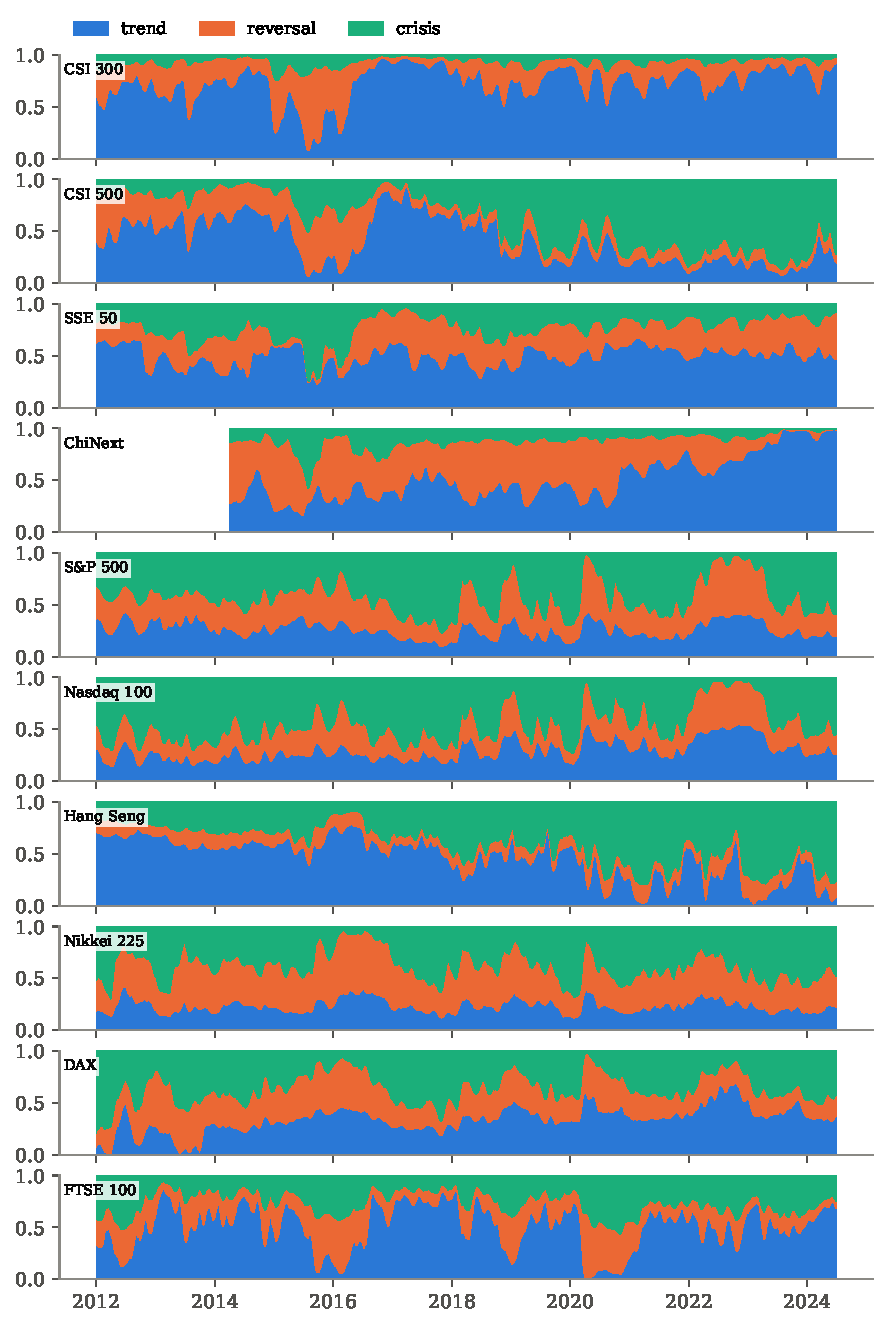
\includegraphics[width=\textwidth,height=0.9\textheight,keepaspectratio]{../results/figures/gates_oos_1.pdf}
\caption{Out-of-sample SMoE gate weights: Chinese and international equity indices.}\label{fig:gates_oos_1}
\end{figure}

\begin{figure}[p]\centering
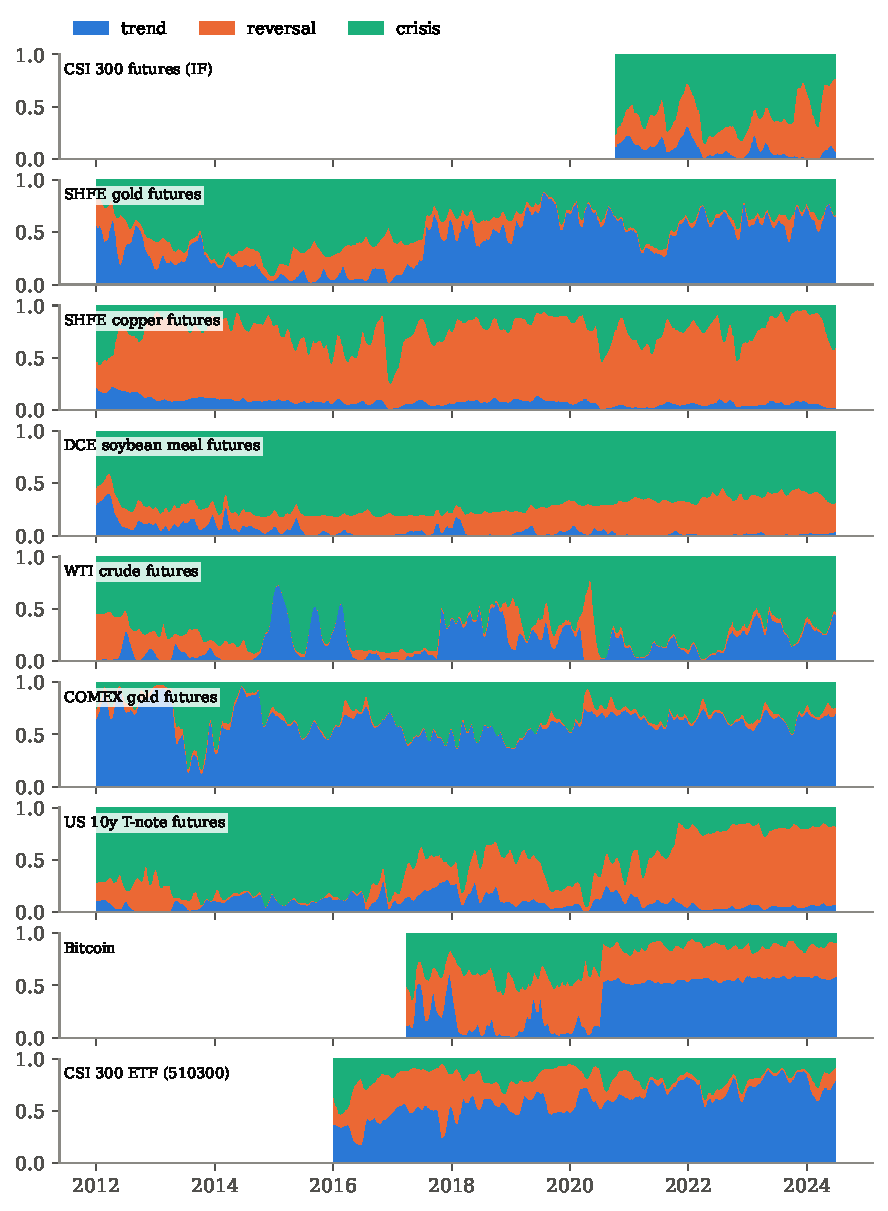
\includegraphics[width=\textwidth,height=0.9\textheight,keepaspectratio]{../results/figures/gates_oos_2.pdf}
\caption{Out-of-sample SMoE gate weights: futures, Bitcoin and the CSI 300 ETF.}\label{fig:gates_oos_2}
\end{figure}

\clearpage
\section{Detailed out-of-sample results by series}\label{app:per-asset}

For every series, the tables report mean losses (lower is better; the best model in bold), the
model-confidence-set $p$-value for log score, the directional hit rate, VaR violation rates with the
Kupiec $p$-value, and the Berkowitz $p$-value of the PIT.

\begin{table}[!htbp]\centering\scriptsize
\caption{Out-of-sample results: CSI 300 ($n=3032$)}\label{tab:asset_csi300}
\begin{adjustbox}{max width=\textwidth}
\begin{tabular}{lrrrrrrrrrrr}
\toprule
Model & NLL & CRPS & QLIKE & FZ5 & Brier & MCS $p$ (NLL) & Hit & Viol 1\% & Viol 5\% & Kupiec 1\% $p$ & Berkowitz $p$\\
\midrule
HistGauss & 1.6889 & 0.7112 & 1.7631 & 1.1842 & 0.2493 & 0.0000 & 0.5261 & 0.0211 & 0.0455 & 0.0000 & 0.0066\\
GARCH-t & 1.5727 & 0.6928 & 1.6004 & 1.0229 & 0.2506 & 0.8920 & 0.5096 & 0.0122 & 0.0485 & 0.2386 & 0.0009\\
AR-GJR-t & 1.5730 & 0.6930 & 1.6007 & 1.0216 & 0.2506 & 0.8290 & 0.5073 & 0.0122 & 0.0482 & 0.2386 & 0.0019\\
Gauss-HAR & 1.5963 & 0.6936 & \textbf{1.5790} & 1.0157 & 0.2502 & 0.0090 & 0.5007 & 0.0191 & 0.0432 & 0.0000 & 0.6238\\
MAR & 1.5783 & 0.6923 & 1.5837 & 1.0300 & 0.2514 & 0.1920 & 0.5125 & 0.0079 & 0.0416 & 0.2313 & 0.6746\\
LSTAR & 1.5722 & 0.6935 & 1.5793 & \textbf{0.9999} & 0.2523 & 0.8920 & 0.5079 & 0.0082 & 0.0429 & 0.3166 & 0.3562\\
MS-AR & 1.6214 & 0.7047 & 1.6868 & 1.0753 & 0.2511 & 0.0000 & 0.4990 & 0.0122 & 0.0402 & 0.2386 & 0.0000\\
XGB-Gauss & 1.6240 & \textbf{0.6904} & 1.6405 & 1.0839 & 0.2492 & 0.0090 & 0.5066 & 0.0297 & 0.0676 & 0.0000 & 0.0000\\
Chronos-Bolt-small & 1.7124 & 0.6982 & 1.8067 & 1.2398 & 0.2506 & 0.0000 & 0.5221 & 0.0359 & 0.0798 & 0.0000 & 0.0000\\
Chronos-Bolt-base & 1.6702 & 0.6964 & 1.7234 & 1.1689 & 0.2500 & 0.0000 & 0.5254 & 0.0307 & 0.0712 & 0.0000 & 0.0000\\
TimesFM-2.5 & 1.6469 & 0.7029 & 1.6648 & 1.1333 & 0.2530 & 0.0000 & 0.4947 & 0.0247 & 0.0590 & 0.0000 & 0.0000\\
Deep-SMoE & \textbf{1.5693} & 0.6908 & 1.5821 & 1.0240 & 0.2496 & 1.0000 & 0.5168 & 0.0102 & 0.0412 & 0.9016 & 0.0200\\
SMoE & 1.5705 & 0.6931 & 1.5831 & 1.0095 & 0.2512 & 0.8920 & 0.5063 & 0.0079 & 0.0416 & 0.2313 & 0.6404\\
\bottomrule
\end{tabular}
\end{adjustbox}
\end{table}
\clearpage
\begin{table}[!htbp]\centering\scriptsize
\caption{Out-of-sample results: CSI 500 ($n=3032$)}\label{tab:asset_csi500}
\begin{adjustbox}{max width=\textwidth}
\begin{tabular}{lrrrrrrrrrrr}
\toprule
Model & NLL & CRPS & QLIKE & FZ5 & Brier & MCS $p$ (NLL) & Hit & Viol 1\% & Viol 5\% & Kupiec 1\% $p$ & Berkowitz $p$\\
\midrule
HistGauss & 1.8334 & 0.8162 & 1.7310 & 1.4251 & 0.2490 & 0.0000 & 0.5234 & 0.0287 & 0.0564 & 0.0000 & 0.0000\\
GARCH-t & 1.7088 & 0.7938 & 1.5461 & 1.2786 & 0.2501 & 0.0010 & 0.5323 & 0.0172 & 0.0623 & 0.0003 & 0.0000\\
AR-GJR-t & 1.7090 & 0.7935 & 1.5473 & 1.2690 & 0.2500 & 0.0010 & 0.5257 & 0.0168 & 0.0623 & 0.0006 & 0.0000\\
Gauss-HAR & 1.7292 & 0.7946 & 1.5230 & 1.2580 & 0.2506 & 0.0000 & 0.5056 & 0.0224 & 0.0511 & 0.0000 & 0.0011\\
MAR & 1.6893 & 0.7887 & 1.5153 & 1.2421 & 0.2493 & 0.0140 & 0.5026 & 0.0073 & 0.0406 & 0.1103 & 0.0078\\
LSTAR & 1.6911 & 0.7892 & 1.5133 & 1.2425 & 0.2505 & 0.0140 & 0.5026 & 0.0089 & 0.0356 & 0.5369 & 0.0017\\
MS-AR & 1.7496 & 0.8083 & 1.6259 & 1.2794 & 0.2507 & 0.0000 & 0.5106 & 0.0132 & 0.0511 & 0.0921 & 0.0000\\
XGB-Gauss & 1.7374 & 0.7881 & 1.5398 & 1.3371 & 0.2484 & 0.0010 & 0.5290 & 0.0317 & 0.0709 & 0.0000 & 0.0000\\
Chronos-Bolt-small & 1.8995 & 0.8025 & 1.8541 & 1.6884 & 0.2502 & 0.0000 & 0.5211 & 0.0554 & 0.1055 & 0.0000 & 0.0000\\
Chronos-Bolt-base & 1.8360 & 0.7974 & 1.7183 & 1.5786 & 0.2494 & 0.0000 & 0.5237 & 0.0439 & 0.0950 & 0.0000 & 0.0000\\
TimesFM-2.5 & 1.8011 & 0.8046 & 1.6493 & 1.4182 & 0.2526 & 0.0000 & 0.5099 & 0.0333 & 0.0762 & 0.0000 & 0.0000\\
Deep-SMoE & \textbf{1.6754} & \textbf{0.7834} & \textbf{1.5080} & \textbf{1.2259} & 0.2462 & 1.0000 & 0.5386 & 0.0082 & 0.0399 & 0.3166 & 0.0000\\
SMoE & 1.6858 & 0.7883 & 1.5103 & 1.2418 & 0.2489 & 0.0140 & 0.5109 & 0.0086 & 0.0429 & 0.4190 & 0.0641\\
\bottomrule
\end{tabular}
\end{adjustbox}
\end{table}
\clearpage
\begin{table}[!htbp]\centering\scriptsize
\caption{Out-of-sample results: SSE 50 ($n=3032$)}\label{tab:asset_sse50}
\begin{adjustbox}{max width=\textwidth}
\begin{tabular}{lrrrrrrrrrrr}
\toprule
Model & NLL & CRPS & QLIKE & FZ5 & Brier & MCS $p$ (NLL) & Hit & Viol 1\% & Viol 5\% & Kupiec 1\% $p$ & Berkowitz $p$\\
\midrule
HistGauss & 1.7067 & 0.7210 & 1.7801 & 1.1624 & 0.2500 & 0.0000 & 0.5122 & 0.0201 & 0.0419 & 0.0000 & 0.0093\\
GARCH-t & 1.5836 & 0.7010 & 1.6209 & 1.0104 & 0.2504 & 0.9110 & 0.4987 & 0.0096 & 0.0468 & 0.8082 & 0.0300\\
AR-GJR-t & 1.5840 & 0.7013 & 1.6215 & 1.0135 & 0.2504 & 0.9110 & 0.4941 & 0.0096 & 0.0462 & 0.8082 & 0.0146\\
Gauss-HAR & 1.6196 & 0.7044 & 1.6073 & 1.0103 & 0.2510 & 0.0010 & 0.4984 & 0.0175 & 0.0432 & 0.0002 & 0.7249\\
MAR & 1.5877 & 0.7012 & 1.6101 & 1.0201 & 0.2511 & 0.5280 & 0.5053 & 0.0112 & 0.0399 & 0.5100 & 0.4513\\
LSTAR & 1.5839 & 0.7022 & 1.6089 & \textbf{0.9950} & 0.2525 & 0.9110 & 0.4967 & 0.0106 & 0.0439 & 0.7612 & 0.3724\\
MS-AR & 1.6296 & 0.7116 & 1.6852 & 1.0614 & 0.2508 & 0.0010 & 0.4911 & 0.0106 & 0.0373 & 0.7612 & 0.0000\\
XGB-Gauss & 1.6529 & \textbf{0.7000} & 1.6785 & 1.0554 & 0.2508 & 0.0010 & 0.5145 & 0.0264 & 0.0663 & 0.0000 & 0.0000\\
Chronos-Bolt-small & 1.7168 & 0.7061 & 1.7997 & 1.1406 & 0.2511 & 0.0000 & 0.5026 & 0.0323 & 0.0768 & 0.0000 & 0.0000\\
Chronos-Bolt-base & 1.6933 & 0.7052 & 1.7524 & 1.1222 & 0.2508 & 0.0000 & 0.5023 & 0.0317 & 0.0699 & 0.0000 & 0.0000\\
TimesFM-2.5 & 1.6678 & 0.7113 & 1.6910 & 1.1106 & 0.2533 & 0.0000 & 0.4891 & 0.0261 & 0.0623 & 0.0000 & 0.0000\\
Deep-SMoE & \textbf{1.5820} & 0.7008 & \textbf{1.6068} & 1.0092 & 0.2515 & 1.0000 & 0.5007 & 0.0109 & 0.0452 & 0.6296 & 0.1319\\
SMoE & 1.5869 & 0.7022 & 1.6181 & 1.0175 & 0.2508 & 0.5710 & 0.5112 & 0.0109 & 0.0419 & 0.6296 & 0.2035\\
\bottomrule
\end{tabular}
\end{adjustbox}
\end{table}
\clearpage
\begin{table}[!htbp]\centering\scriptsize
\caption{Out-of-sample results: ChiNext ($n=2306$)}\label{tab:asset_chinext}
\begin{adjustbox}{max width=\textwidth}
\begin{tabular}{lrrrrrrrrrrr}
\toprule
Model & NLL & CRPS & QLIKE & FZ5 & Brier & MCS $p$ (NLL) & Hit & Viol 1\% & Viol 5\% & Kupiec 1\% $p$ & Berkowitz $p$\\
\midrule
HistGauss & 2.0278 & 1.0167 & 1.5820 & 1.4970 & 0.2493 & 0.0000 & 0.5312 & 0.0234 & 0.0516 & 0.0000 & 0.0012\\
GARCH-t & 1.9335 & 0.9910 & 1.4222 & 1.3746 & 0.2504 & 0.9130 & 0.4931 & 0.0139 & 0.0546 & 0.0772 & 0.2867\\
AR-GJR-t & 1.9353 & 0.9927 & 1.4245 & \textbf{1.3635} & 0.2519 & 0.5930 & 0.4696 & 0.0130 & 0.0542 & 0.1651 & 0.3199\\
Gauss-HAR & 1.9421 & 0.9912 & 1.4095 & 1.3688 & 0.2517 & 0.4580 & 0.4935 & 0.0165 & 0.0460 & 0.0042 & 0.4531\\
MAR & \textbf{1.9306} & \textbf{0.9882} & \textbf{1.4025} & 1.3665 & 0.2519 & 1.0000 & 0.5056 & 0.0078 & 0.0442 & 0.2707 & 0.9335\\
LSTAR & 1.9313 & 0.9900 & 1.4085 & 1.3725 & 0.2517 & 0.9200 & 0.5061 & 0.0108 & 0.0399 & 0.6887 & 0.5788\\
MS-AR & 1.9854 & 1.0093 & 1.5185 & 1.4284 & 0.2523 & 0.0010 & 0.4653 & 0.0143 & 0.0464 & 0.0507 & 0.0374\\
XGB-Gauss & 1.9537 & 0.9922 & 1.4316 & 1.4071 & 0.2505 & 0.0760 & 0.5191 & 0.0225 & 0.0564 & 0.0000 & 0.0000\\
Chronos-Bolt-small & 2.0678 & 1.0027 & 1.6561 & 1.5865 & 0.2533 & 0.0000 & 0.5013 & 0.0390 & 0.0846 & 0.0000 & 0.0000\\
Chronos-Bolt-base & 2.0112 & 0.9942 & 1.5433 & 1.4946 & 0.2509 & 0.0010 & 0.5199 & 0.0304 & 0.0733 & 0.0000 & 0.0000\\
Deep-SMoE & 1.9327 & 0.9945 & 1.4131 & 1.3695 & 0.2522 & 0.9200 & 0.5169 & 0.0095 & 0.0455 & 0.8231 & 0.8796\\
SMoE & 1.9380 & 0.9936 & 1.4148 & 1.3798 & 0.2529 & 0.4580 & 0.4974 & 0.0091 & 0.0455 & 0.6616 & 0.7625\\
\bottomrule
\end{tabular}
\end{adjustbox}
\end{table}
\clearpage
\begin{table}[!htbp]\centering\scriptsize
\caption{Out-of-sample results: S\&P 500 ($n=3142$)}\label{tab:asset_spx}
\begin{adjustbox}{max width=\textwidth}
\begin{tabular}{lrrrrrrrrrrr}
\toprule
Model & NLL & CRPS & QLIKE & FZ5 & Brier & MCS $p$ (NLL) & Hit & Viol 1\% & Viol 5\% & Kupiec 1\% $p$ & Berkowitz $p$\\
\midrule
HistGauss & 1.4202 & 0.5299 & 1.9518 & 0.9700 & 0.2486 & 0.0000 & 0.5331 & 0.0258 & 0.0522 & 0.0000 & 0.0030\\
GARCH-t & 1.2144 & 0.5018 & 1.6039 & 0.7313 & 0.2487 & 0.0010 & 0.5411 & 0.0156 & 0.0602 & 0.0036 & 0.0337\\
AR-GJR-t & 1.1968 & 0.4976 & 1.5811 & 0.7173 & 0.2484 & 0.2460 & 0.5423 & 0.0134 & 0.0592 & 0.0712 & 0.3116\\
Gauss-HAR & 1.2216 & 0.4999 & 1.5554 & 0.7297 & 0.2491 & 0.0010 & 0.5236 & 0.0223 & 0.0547 & 0.0000 & 0.0068\\
MAR & 1.1828 & 0.4974 & 1.5284 & 0.6767 & 0.2490 & 0.2500 & 0.5271 & 0.0108 & 0.0452 & 0.6480 & 0.0214\\
LSTAR & 1.1923 & 0.4995 & 1.5492 & 0.7002 & 0.2494 & 0.2460 & 0.5220 & 0.0121 & 0.0474 & 0.2534 & 0.0056\\
MS-AR & 1.2795 & 0.5126 & 1.7061 & 0.7899 & 0.2482 & 0.0000 & 0.5328 & 0.0124 & 0.0506 & 0.1903 & 0.0000\\
XGB-Gauss & 1.2615 & 0.5022 & 1.6355 & 0.8205 & 0.2494 & 0.0000 & 0.5130 & 0.0353 & 0.0789 & 0.0000 & 0.0000\\
Chronos-Bolt-small & 1.4465 & 0.5150 & 1.9913 & 1.1673 & 0.2498 & 0.0000 & 0.5395 & 0.0519 & 0.0990 & 0.0000 & 0.0000\\
Chronos-Bolt-base & 1.3594 & 0.5109 & 1.8170 & 1.0271 & 0.2497 & 0.0000 & 0.5391 & 0.0471 & 0.0885 & 0.0000 & 0.0000\\
TimesFM-2.5 & 1.3677 & 0.5183 & 1.8147 & 0.9725 & 0.2528 & 0.0000 & 0.5178 & 0.0407 & 0.0815 & 0.0000 & 0.0000\\
Deep-SMoE & 1.1914 & 0.5004 & 1.5450 & 0.6965 & 0.2502 & 0.2460 & 0.5029 & 0.0115 & 0.0490 & 0.4222 & 0.0094\\
SMoE & \textbf{1.1802} & \textbf{0.4970} & \textbf{1.5235} & \textbf{0.6739} & 0.2492 & 1.0000 & 0.5216 & 0.0102 & 0.0411 & 0.9174 & 0.0459\\
\bottomrule
\end{tabular}
\end{adjustbox}
\end{table}
\clearpage
\begin{table}[!htbp]\centering\scriptsize
\caption{Out-of-sample results: Nasdaq 100 ($n=3142$)}\label{tab:asset_ndx}
\begin{adjustbox}{max width=\textwidth}
\begin{tabular}{lrrrrrrrrrrr}
\toprule
Model & NLL & CRPS & QLIKE & FZ5 & Brier & MCS $p$ (NLL) & Hit & Viol 1\% & Viol 5\% & Kupiec 1\% $p$ & Berkowitz $p$\\
\midrule
HistGauss & 1.6258 & 0.6666 & 1.7879 & 1.1522 & 0.2477 & 0.0000 & 0.5477 & 0.0251 & 0.0560 & 0.0000 & 0.0004\\
GARCH-t & 1.4779 & 0.6427 & 1.5404 & 0.9714 & 0.2471 & 0.0000 & 0.5538 & 0.0153 & 0.0643 & 0.0058 & 0.0801\\
AR-GJR-t & 1.4635 & 0.6385 & 1.5176 & 0.9593 & 0.2475 & 0.0030 & 0.5557 & 0.0156 & 0.0595 & 0.0036 & 0.7861\\
Gauss-HAR & 1.4744 & 0.6394 & 1.4874 & 0.9435 & 0.2490 & 0.0000 & 0.5356 & 0.0242 & 0.0598 & 0.0000 & 0.0133\\
MAR & 1.4468 & 0.6368 & 1.4721 & \textbf{0.9040} & 0.2474 & 0.1130 & 0.5363 & 0.0111 & 0.0525 & 0.5285 & 0.0198\\
LSTAR & 1.4486 & 0.6375 & 1.4821 & 0.9155 & 0.2481 & 0.1130 & 0.5318 & 0.0130 & 0.0528 & 0.1009 & 0.0113\\
MS-AR & 1.5207 & 0.6509 & 1.6154 & 1.0051 & 0.2476 & 0.0000 & 0.5363 & 0.0169 & 0.0544 & 0.0004 & 0.0027\\
XGB-Gauss & 1.4956 & 0.6406 & 1.5305 & 0.9977 & 0.2486 & 0.0000 & 0.5465 & 0.0315 & 0.0764 & 0.0000 & 0.0000\\
Chronos-Bolt-small & 1.6692 & 0.6556 & 1.8643 & 1.3830 & 0.2486 & 0.0000 & 0.5420 & 0.0519 & 0.1015 & 0.0000 & 0.0000\\
Chronos-Bolt-base & 1.6013 & 0.6514 & 1.7290 & 1.2519 & 0.2484 & 0.0000 & 0.5465 & 0.0446 & 0.0913 & 0.0000 & 0.0000\\
TimesFM-2.5 & 1.6055 & 0.6575 & 1.7200 & 1.2258 & 0.2501 & 0.0000 & 0.5391 & 0.0420 & 0.0878 & 0.0000 & 0.0000\\
Deep-SMoE & \textbf{1.4394} & 0.6376 & \textbf{1.4600} & 0.9067 & 0.2481 & 1.0000 & 0.5169 & 0.0121 & 0.0554 & 0.2534 & 0.0125\\
SMoE & 1.4414 & \textbf{0.6361} & 1.4652 & 0.9050 & 0.2478 & 0.6980 & 0.5232 & 0.0111 & 0.0500 & 0.5285 & 0.0399\\
\bottomrule
\end{tabular}
\end{adjustbox}
\end{table}
\clearpage
\begin{table}[!htbp]\centering\scriptsize
\caption{Out-of-sample results: Hang Seng ($n=3072$)}\label{tab:asset_hsi}
\begin{adjustbox}{max width=\textwidth}
\begin{tabular}{lrrrrrrrrrrr}
\toprule
Model & NLL & CRPS & QLIKE & FZ5 & Brier & MCS $p$ (NLL) & Hit & Viol 1\% & Viol 5\% & Kupiec 1\% $p$ & Berkowitz $p$\\
\midrule
HistGauss & 1.6371 & 0.6787 & 1.6393 & 1.0697 & 0.2500 & 0.0000 & 0.5062 & 0.0208 & 0.0475 & 0.0000 & 0.1119\\
GARCH-t & 1.5682 & 0.6706 & 1.5350 & 1.0025 & 0.2500 & 0.1420 & 0.5107 & 0.0153 & 0.0605 & 0.0062 & 0.0031\\
AR-GJR-t & 1.5624 & \textbf{0.6687} & 1.5218 & 0.9848 & 0.2499 & 0.8240 & 0.5111 & 0.0130 & 0.0576 & 0.1078 & 0.0331\\
Gauss-HAR & 1.5821 & 0.6724 & 1.5312 & 0.9878 & 0.2502 & 0.0000 & 0.5026 & 0.0160 & 0.0472 & 0.0023 & 0.0001\\
MAR & 1.5613 & 0.6692 & 1.5173 & 0.9683 & 0.2502 & 0.8240 & 0.4984 & 0.0094 & 0.0426 & 0.7529 & 0.0028\\
LSTAR & 1.5704 & 0.6710 & 1.5263 & 0.9804 & 0.2508 & 0.0200 & 0.5003 & 0.0114 & 0.0452 & 0.4477 & 0.0011\\
MS-AR & 1.6011 & 0.6780 & 1.5955 & 1.0435 & 0.2499 & 0.0000 & 0.5049 & 0.0153 & 0.0625 & 0.0062 & 0.0585\\
XGB-Gauss & 1.5858 & 0.6695 & 1.5361 & 1.0200 & 0.2501 & 0.0020 & 0.5238 & 0.0218 & 0.0638 & 0.0000 & 0.0000\\
Chronos-Bolt-small & 1.6793 & 0.6775 & 1.7152 & 1.2155 & 0.2513 & 0.0000 & 0.5085 & 0.0407 & 0.0905 & 0.0000 & 0.0000\\
Chronos-Bolt-base & 1.6414 & 0.6750 & 1.6411 & 1.1414 & 0.2507 & 0.0000 & 0.5052 & 0.0329 & 0.0801 & 0.0000 & 0.0000\\
Deep-SMoE & 1.5626 & 0.6704 & 1.5189 & \textbf{0.9596} & 0.2504 & 0.8240 & 0.5026 & 0.0065 & 0.0420 & 0.0379 & 0.0000\\
SMoE & \textbf{1.5582} & 0.6687 & \textbf{1.5092} & 0.9697 & 0.2505 & 1.0000 & 0.5059 & 0.0094 & 0.0417 & 0.7529 & 0.0011\\
\bottomrule
\end{tabular}
\end{adjustbox}
\end{table}
\clearpage
\begin{table}[!htbp]\centering\scriptsize
\caption{Out-of-sample results: Nikkei 225 ($n=3057$)}\label{tab:asset_n225}
\begin{adjustbox}{max width=\textwidth}
\begin{tabular}{lrrrrrrrrrrr}
\toprule
Model & NLL & CRPS & QLIKE & FZ5 & Brier & MCS $p$ (NLL) & Hit & Viol 1\% & Viol 5\% & Kupiec 1\% $p$ & Berkowitz $p$\\
\midrule
HistGauss & 1.6697 & 0.6845 & 1.7130 & 1.1422 & 0.2501 & 0.0000 & 0.5067 & 0.0206 & 0.0556 & 0.0000 & 0.0324\\
GARCH-t & 1.5622 & 0.6685 & 1.5393 & 1.0243 & 0.2491 & 0.0850 & 0.5345 & 0.0150 & 0.0582 & 0.0091 & 0.1068\\
AR-GJR-t & 1.5533 & \textbf{0.6658} & 1.5216 & 0.9977 & 0.2492 & 0.8860 & 0.5335 & 0.0141 & 0.0569 & 0.0333 & 0.2601\\
Gauss-HAR & 1.5737 & 0.6691 & 1.5225 & 1.0120 & 0.2501 & 0.0000 & 0.5018 & 0.0170 & 0.0474 & 0.0004 & 0.2177\\
MAR & 1.5513 & 0.6671 & 1.5068 & 1.0095 & 0.2506 & 0.8860 & 0.5005 & 0.0101 & 0.0425 & 0.9378 & 0.2270\\
LSTAR & 1.5595 & 0.6668 & 1.5116 & 1.0097 & 0.2501 & 0.0850 & 0.5067 & 0.0121 & 0.0429 & 0.2579 & 0.2206\\
MS-AR & 1.5918 & 0.6762 & 1.5893 & 1.0367 & 0.2493 & 0.0000 & 0.5293 & 0.0114 & 0.0491 & 0.4312 & 0.0000\\
XGB-Gauss & 1.5848 & 0.6673 & 1.5448 & 1.0528 & 0.2500 & 0.0000 & 0.5129 & 0.0252 & 0.0648 & 0.0000 & 0.0000\\
Chronos-Bolt-small & 1.7093 & 0.6779 & 1.7884 & 1.2607 & 0.2506 & 0.0000 & 0.5132 & 0.0461 & 0.0926 & 0.0000 & 0.0000\\
Chronos-Bolt-base & 1.6538 & 0.6738 & 1.6806 & 1.1772 & 0.2502 & 0.0000 & 0.5146 & 0.0386 & 0.0831 & 0.0000 & 0.0000\\
TimesFM-2.5 & 1.6418 & 0.6791 & 1.6401 & 1.1366 & 0.2523 & 0.0000 & 0.5110 & 0.0307 & 0.0729 & 0.0000 & 0.0000\\
Deep-SMoE & \textbf{1.5492} & 0.6663 & 1.5072 & \textbf{0.9851} & 0.2507 & 1.0000 & 0.4920 & 0.0098 & 0.0432 & 0.9172 & 0.0874\\
SMoE & 1.5533 & 0.6660 & \textbf{1.5038} & 1.0052 & 0.2501 & 0.8860 & 0.5005 & 0.0121 & 0.0429 & 0.2579 & 0.3680\\
\bottomrule
\end{tabular}
\end{adjustbox}
\end{table}
\clearpage
\begin{table}[!htbp]\centering\scriptsize
\caption{Out-of-sample results: DAX ($n=3166$)}\label{tab:asset_dax}
\begin{adjustbox}{max width=\textwidth}
\begin{tabular}{lrrrrrrrrrrr}
\toprule
Model & NLL & CRPS & QLIKE & FZ5 & Brier & MCS $p$ (NLL) & Hit & Viol 1\% & Viol 5\% & Kupiec 1\% $p$ & Berkowitz $p$\\
\midrule
HistGauss & 1.5740 & 0.6248 & 1.7686 & 1.0643 & 0.2499 & 0.0040 & 0.5123 & 0.0202 & 0.0581 & 0.0000 & 0.8871\\
GARCH-t & 1.4430 & 0.6045 & 1.5704 & 0.9493 & 0.2488 & 0.0110 & 0.5376 & 0.0142 & 0.0654 & 0.0250 & 0.0007\\
AR-GJR-t & 1.4272 & 0.6006 & 1.5406 & 0.9245 & 0.2487 & 0.5040 & 0.5379 & 0.0139 & 0.0600 & 0.0374 & 0.0252\\
Gauss-HAR & 1.4551 & 0.6022 & 1.5348 & 0.9445 & 0.2489 & 0.0110 & 0.5379 & 0.0218 & 0.0603 & 0.0000 & 0.2470\\
MAR & 1.4263 & 0.5995 & 1.5160 & 0.9090 & 0.2480 & 0.5040 & 0.5306 & 0.0133 & 0.0461 & 0.0786 & 0.2814\\
LSTAR & 1.4315 & 0.6004 & 1.5237 & 0.9106 & 0.2484 & 0.1730 & 0.5363 & 0.0139 & 0.0524 & 0.0374 & 0.0229\\
MS-AR & 1.4910 & 0.6137 & 1.6368 & 0.9856 & 0.2490 & 0.0040 & 0.5275 & 0.0148 & 0.0553 & 0.0106 & 0.0000\\
XGB-Gauss & 1.4762 & 0.6023 & 1.5766 & 1.0174 & 0.2493 & 0.0110 & 0.5357 & 0.0322 & 0.0771 & 0.0000 & 0.0000\\
Chronos-Bolt-small & 1.6405 & 0.6142 & 1.8885 & 1.3063 & 0.2512 & 0.0010 & 0.5171 & 0.0493 & 0.1036 & 0.0000 & 0.0000\\
Chronos-Bolt-base & 1.5828 & 0.6119 & 1.7752 & 1.1897 & 0.2509 & 0.0110 & 0.5167 & 0.0436 & 0.0970 & 0.0000 & 0.0000\\
TimesFM-2.5 & 1.5463 & 0.6173 & 1.6939 & 1.0907 & 0.2529 & 0.0010 & 0.5123 & 0.0366 & 0.0821 & 0.0000 & 0.0000\\
Deep-SMoE & \textbf{1.4139} & \textbf{0.5992} & \textbf{1.5084} & \textbf{0.8970} & 0.2493 & 1.0000 & 0.5069 & 0.0136 & 0.0499 & 0.0548 & 0.9739\\
SMoE & 1.4258 & 0.5998 & 1.5124 & 0.9067 & 0.2484 & 0.5040 & 0.5268 & 0.0130 & 0.0442 & 0.1106 & 0.3683\\
\bottomrule
\end{tabular}
\end{adjustbox}
\end{table}
\clearpage
\begin{table}[!htbp]\centering\scriptsize
\caption{Out-of-sample results: FTSE 100 ($n=3153$)}\label{tab:asset_ftse}
\begin{adjustbox}{max width=\textwidth}
\begin{tabular}{lrrrrrrrrrrr}
\toprule
Model & NLL & CRPS & QLIKE & FZ5 & Brier & MCS $p$ (NLL) & Hit & Viol 1\% & Viol 5\% & Kupiec 1\% $p$ & Berkowitz $p$\\
\midrule
HistGauss & 1.3456 & 0.4961 & 1.7771 & 0.8558 & 0.2502 & 0.0020 & 0.5075 & 0.0206 & 0.0533 & 0.0000 & 0.8978\\
GARCH-t & 1.2107 & 0.4800 & 1.5670 & 0.7237 & 0.2498 & 0.0020 & 0.5281 & 0.0174 & 0.0571 & 0.0001 & 0.0005\\
AR-GJR-t & 1.1962 & 0.4774 & 1.5300 & 0.6938 & 0.2498 & 0.6460 & 0.5230 & 0.0165 & 0.0558 & 0.0008 & 0.0007\\
Gauss-HAR & 1.2204 & 0.4793 & 1.5295 & 0.7165 & 0.2501 & 0.0020 & 0.5144 & 0.0212 & 0.0552 & 0.0000 & 0.2965\\
MAR & 1.1952 & 0.4771 & 1.5074 & \textbf{0.6767} & 0.2500 & 0.6460 & 0.5135 & 0.0133 & 0.0457 & 0.0745 & 0.1201\\
LSTAR & 1.2016 & 0.4780 & 1.5163 & 0.6972 & 0.2507 & 0.0270 & 0.5103 & 0.0136 & 0.0441 & 0.0517 & 0.0097\\
MS-AR & 1.2471 & 0.4867 & 1.6200 & 0.7519 & 0.2504 & 0.0020 & 0.5075 & 0.0127 & 0.0517 & 0.1456 & 0.0000\\
XGB-Gauss & 1.2265 & 0.4788 & 1.5399 & 0.7416 & 0.2503 & 0.0020 & 0.5179 & 0.0282 & 0.0650 & 0.0000 & 0.0000\\
Chronos-Bolt-small & 1.3993 & 0.4875 & 1.8778 & 1.0288 & 0.2502 & 0.0010 & 0.5312 & 0.0460 & 0.0990 & 0.0000 & 0.0000\\
Chronos-Bolt-base & 1.3482 & 0.4868 & 1.7698 & 0.9652 & 0.2515 & 0.0020 & 0.5081 & 0.0412 & 0.0885 & 0.0000 & 0.0000\\
Deep-SMoE & \textbf{1.1908} & 0.4767 & 1.5095 & 0.6769 & 0.2504 & 1.0000 & 0.5154 & 0.0121 & 0.0473 & 0.2619 & 0.0201\\
SMoE & 1.1913 & \textbf{0.4761} & \textbf{1.5060} & 0.6989 & 0.2491 & 0.9370 & 0.5103 & 0.0127 & 0.0409 & 0.1456 & 0.0001\\
\bottomrule
\end{tabular}
\end{adjustbox}
\end{table}
\clearpage
\begin{table}[!htbp]\centering\scriptsize
\caption{Out-of-sample results: CSI 300 futures (IF) ($n=844$)}\label{tab:asset_if_main}
\begin{adjustbox}{max width=\textwidth}
\begin{tabular}{lrrrrrrrrrrr}
\toprule
Model & NLL & CRPS & QLIKE & FZ5 & Brier & MCS $p$ (NLL) & Hit & Viol 1\% & Viol 5\% & Kupiec 1\% $p$ & Berkowitz $p$\\
\midrule
HistGauss & 1.5261 & 0.6068 & 1.5864 & 0.9338 & 0.2498 & 0.1600 & 0.5213 & 0.0130 & 0.0367 & 0.3975 & 0.3007\\
GARCH-t & 1.4789 & 0.6020 & 1.5230 & 0.8709 & 0.2521 & 0.9260 & 0.4502 & 0.0047 & 0.0474 & 0.0869 & 0.0114\\
AR-GJR-t & \textbf{1.4756} & \textbf{0.6012} & 1.5159 & 0.8676 & 0.2517 & 1.0000 & 0.4799 & 0.0047 & 0.0438 & 0.0869 & 0.0119\\
Gauss-HAR & 1.4952 & 0.6069 & 1.5224 & \textbf{0.8608} & 0.2511 & 0.3240 & 0.4834 & 0.0083 & 0.0355 & 0.6077 & 0.0001\\
MAR & 1.4880 & 0.6030 & 1.5314 & 0.8880 & 0.2522 & 0.8010 & 0.5118 & 0.0083 & 0.0391 & 0.6077 & 0.0066\\
LSTAR & 1.4838 & 0.6030 & 1.5202 & 0.8766 & 0.2524 & 0.9260 & 0.5095 & 0.0071 & 0.0403 & 0.3734 & 0.0026\\
MS-AR & 1.4857 & 0.6052 & 1.5374 & 0.8680 & 0.2526 & 0.9260 & 0.4562 & 0.0071 & 0.0403 & 0.3734 & 0.0005\\
XGB-Gauss & 1.4873 & 0.6015 & \textbf{1.5030} & 0.8873 & 0.2520 & 0.9260 & 0.4680 & 0.0201 & 0.0581 & 0.0092 & 0.0071\\
Chronos-Bolt-small & 1.5709 & 0.6052 & 1.6750 & 1.0121 & 0.2496 & 0.0440 & 0.5415 & 0.0344 & 0.0746 & 0.0000 & 0.0000\\
Chronos-Bolt-base & 1.5514 & 0.6050 & 1.6334 & 0.9831 & 0.2504 & 0.0920 & 0.5166 & 0.0320 & 0.0640 & 0.0000 & 0.0000\\
Deep-SMoE & 1.4793 & 0.6053 & 1.5245 & 0.8668 & 0.2537 & 0.9260 & 0.4585 & 0.0047 & 0.0367 & 0.0869 & 0.0000\\
SMoE & 1.4852 & 0.6021 & 1.5203 & 0.8747 & 0.2521 & 0.9260 & 0.5166 & 0.0083 & 0.0379 & 0.6077 & 0.0029\\
\bottomrule
\end{tabular}
\end{adjustbox}
\end{table}
\clearpage
\begin{table}[!htbp]\centering\scriptsize
\caption{Out-of-sample results: SHFE gold futures ($n=3036$)}\label{tab:asset_au_main}
\begin{adjustbox}{max width=\textwidth}
\begin{tabular}{lrrrrrrrrrrr}
\toprule
Model & NLL & CRPS & QLIKE & FZ5 & Brier & MCS $p$ (NLL) & Hit & Viol 1\% & Viol 5\% & Kupiec 1\% $p$ & Berkowitz $p$\\
\midrule
HistGauss & 1.2709 & 0.4624 & 1.9341 & 0.6888 & 0.2497 & 0.0080 & 0.5175 & 0.0181 & 0.0418 & 0.0001 & 0.3901\\
GARCH-t & \textbf{1.1664} & \textbf{0.4547} & \textbf{1.8290} & \textbf{0.6188} & 0.2502 & 1.0000 & 0.5122 & 0.0096 & 0.0448 & 0.8026 & 0.0653\\
AR-GJR-t & 1.1671 & 0.4548 & 1.8349 & 0.6348 & 0.2500 & 0.6560 & 0.5158 & 0.0099 & 0.0478 & 0.9475 & 0.0022\\
Gauss-HAR & 1.3518 & 0.4850 & 2.0852 & 0.8251 & 0.2495 & 0.0000 & 0.5175 & 0.0063 & 0.0188 & 0.0260 & 0.0000\\
MAR & 1.2302 & 0.4653 & 2.0683 & 0.8137 & 0.2497 & 0.0570 & 0.5198 & 0.0023 & 0.0181 & 0.0000 & 0.0000\\
LSTAR & 1.2365 & 0.4665 & 2.0554 & 0.8167 & 0.2496 & 0.0160 & 0.5161 & 0.0026 & 0.0175 & 0.0000 & 0.0000\\
MS-AR & 1.2160 & 0.4624 & 1.9108 & 0.6616 & 0.2500 & 0.0780 & 0.5184 & 0.0076 & 0.0329 & 0.1608 & 0.0000\\
XGB-Gauss & 1.3023 & 0.4636 & 1.9885 & 0.7344 & 0.2502 & 0.0780 & 0.5099 & 0.0125 & 0.0336 & 0.1799 & 0.0000\\
Chronos-Bolt-small & 1.3356 & 0.4595 & 2.0630 & 0.7701 & 0.2516 & 0.0020 & 0.5105 & 0.0356 & 0.0800 & 0.0000 & 0.0000\\
Chronos-Bolt-base & 1.3016 & 0.4573 & 2.0012 & 0.7388 & 0.2503 & 0.0060 & 0.5217 & 0.0352 & 0.0708 & 0.0000 & 0.0000\\
Deep-SMoE & 1.2507 & 0.4728 & 2.0143 & 0.7658 & 0.2505 & 0.0210 & 0.5168 & 0.0053 & 0.0208 & 0.0040 & 0.0000\\
SMoE & 1.2168 & 0.4641 & 1.9782 & 0.7452 & 0.2501 & 0.0780 & 0.5072 & 0.0043 & 0.0247 & 0.0004 & 0.0000\\
\bottomrule
\end{tabular}
\end{adjustbox}
\end{table}
\clearpage
\begin{table}[!htbp]\centering\scriptsize
\caption{Out-of-sample results: SHFE copper futures ($n=3033$)}\label{tab:asset_cu_main}
\begin{adjustbox}{max width=\textwidth}
\begin{tabular}{lrrrrrrrrrrr}
\toprule
Model & NLL & CRPS & QLIKE & FZ5 & Brier & MCS $p$ (NLL) & Hit & Viol 1\% & Viol 5\% & Kupiec 1\% $p$ & Berkowitz $p$\\
\midrule
HistGauss & 1.5387 & 0.5893 & 1.9274 & 0.9991 & 0.2503 & 0.0040 & 0.5124 & 0.0165 & 0.0419 & 0.0010 & 0.2716\\
GARCH-t & 1.4127 & 0.5764 & 1.7654 & \textbf{0.8592} & 0.2502 & 0.0460 & 0.5051 & 0.0082 & 0.0439 & 0.3158 & 0.0003\\
AR-GJR-t & \textbf{1.4091} & \textbf{0.5749} & \textbf{1.7630} & 0.8627 & 0.2492 & 1.0000 & 0.5325 & 0.0073 & 0.0439 & 0.1100 & 0.0000\\
Gauss-HAR & 1.5069 & 0.5983 & 1.8611 & 0.9344 & 0.2507 & 0.0020 & 0.5058 & 0.0066 & 0.0227 & 0.0445 & 0.0000\\
MAR & 1.4298 & 0.5828 & 1.8169 & 0.9156 & 0.2500 & 0.0180 & 0.5054 & 0.0020 & 0.0185 & 0.0000 & 0.0000\\
LSTAR & 1.4391 & 0.5863 & 1.8342 & 0.9279 & 0.2501 & 0.0180 & 0.5064 & 0.0016 & 0.0221 & 0.0000 & 0.0000\\
MS-AR & 1.4579 & 0.5848 & 1.8201 & 0.8818 & 0.2494 & 0.0090 & 0.5223 & 0.0069 & 0.0359 & 0.0715 & 0.0000\\
XGB-Gauss & 1.4677 & 0.5826 & 1.7852 & 0.8828 & 0.2508 & 0.0180 & 0.5061 & 0.0135 & 0.0386 & 0.0646 & 0.0053\\
Chronos-Bolt-small & 1.6114 & 0.5831 & 2.0784 & 1.0881 & 0.2523 & 0.0020 & 0.4988 & 0.0369 & 0.0798 & 0.0000 & 0.0000\\
Chronos-Bolt-base & 1.5572 & 0.5805 & 1.9676 & 1.0020 & 0.2514 & 0.0090 & 0.4906 & 0.0310 & 0.0712 & 0.0000 & 0.0000\\
Deep-SMoE & 1.4358 & 0.5850 & 1.8059 & 0.8862 & 0.2518 & 0.0180 & 0.4870 & 0.0026 & 0.0237 & 0.0000 & 0.0000\\
SMoE & 1.4218 & 0.5811 & 1.8026 & 0.8792 & 0.2499 & 0.0460 & 0.5163 & 0.0026 & 0.0267 & 0.0000 & 0.0000\\
\bottomrule
\end{tabular}
\end{adjustbox}
\end{table}
\clearpage
\begin{table}[!htbp]\centering\scriptsize
\caption{Out-of-sample results: DCE soybean meal futures ($n=3032$)}\label{tab:asset_m_main}
\begin{adjustbox}{max width=\textwidth}
\begin{tabular}{lrrrrrrrrrrr}
\toprule
Model & NLL & CRPS & QLIKE & FZ5 & Brier & MCS $p$ (NLL) & Hit & Viol 1\% & Viol 5\% & Kupiec 1\% $p$ & Berkowitz $p$\\
\midrule
HistGauss & 1.8308 & 0.7416 & 2.2110 & 1.3053 & 0.2506 & 0.0000 & 0.4921 & 0.0165 & 0.0363 & 0.0010 & 0.0958\\
GARCH-t & 1.6408 & 0.7243 & 2.1896 & 1.2332 & 0.2501 & 0.3640 & 0.5007 & 0.0102 & 0.0425 & 0.9016 & 0.3011\\
AR-GJR-t & \textbf{1.6336} & 0.7221 & \textbf{2.1458} & \textbf{1.2132} & 0.2503 & 1.0000 & 0.5165 & 0.0099 & 0.0412 & 0.9533 & 0.0032\\
Gauss-HAR & 1.8224 & 0.7391 & 2.2002 & 1.2890 & 0.2498 & 0.0000 & 0.5102 & 0.0129 & 0.0247 & 0.1292 & 0.0000\\
MAR & 1.6471 & \textbf{0.7207} & 2.1881 & 1.2603 & 0.2498 & 0.2920 & 0.5175 & 0.0096 & 0.0303 & 0.8082 & 0.0000\\
LSTAR & 1.6638 & 0.7243 & 2.2153 & 1.2359 & 0.2499 & 0.0060 & 0.5168 & 0.0089 & 0.0369 & 0.5369 & 0.0000\\
MS-AR & 1.6674 & 0.7247 & 2.1680 & 1.2412 & 0.2500 & 0.0060 & 0.5122 & 0.0106 & 0.0465 & 0.7612 & 0.0606\\
XGB-Gauss & 1.8783 & 0.7212 & 2.3112 & 1.3158 & 0.2504 & 0.0000 & 0.5106 & 0.0175 & 0.0511 & 0.0002 & 0.0000\\
Chronos-Bolt-small & 2.0641 & 0.7271 & 2.6815 & 1.4648 & 0.2521 & 0.0000 & 0.4888 & 0.0379 & 0.0834 & 0.0000 & 0.0000\\
Chronos-Bolt-base & 1.9815 & 0.7232 & 2.5204 & 1.4002 & 0.2512 & 0.0000 & 0.4980 & 0.0307 & 0.0749 & 0.0000 & 0.0000\\
TimesFM-2.5 & 1.9232 & 0.7302 & 2.3857 & 1.3710 & 0.2556 & 0.0000 & 0.4911 & 0.0297 & 0.0752 & 0.0000 & 0.0000\\
Deep-SMoE & 1.6716 & 0.7241 & 2.1884 & 1.2570 & 0.2499 & 0.0010 & 0.5181 & 0.0106 & 0.0310 & 0.7612 & 0.0000\\
SMoE & 1.6457 & 0.7208 & 2.2229 & 1.2591 & 0.2497 & 0.3640 & 0.5214 & 0.0112 & 0.0353 & 0.5100 & 0.0000\\
\bottomrule
\end{tabular}
\end{adjustbox}
\end{table}
\clearpage
\begin{table}[!htbp]\centering\scriptsize
\caption{Out-of-sample results: WTI crude futures ($n=3139$)}\label{tab:asset_cl_fut}
\begin{adjustbox}{max width=\textwidth}
\begin{tabular}{lrrrrrrrrrrr}
\toprule
Model & NLL & CRPS & QLIKE & FZ5 & Brier & MCS $p$ (NLL) & Hit & Viol 1\% & Viol 5\% & Kupiec 1\% $p$ & Berkowitz $p$\\
\midrule
HistGauss & 2.3302 & 1.3277 & 1.8845 & 1.8180 & 0.2494 & 0.0030 & 0.5148 & 0.0210 & 0.0529 & 0.0000 & 0.0000\\
GARCH-t & 2.1266 & 1.2609 & 1.5498 & 1.6397 & 0.2497 & 0.0970 & 0.5237 & 0.0153 & 0.0615 & 0.0057 & 0.2029\\
AR-GJR-t & 2.1244 & 1.2608 & 1.5320 & 1.6164 & 0.2497 & 0.2830 & 0.5126 & 0.0140 & 0.0561 & 0.0329 & 0.1832\\
Gauss-HAR & 2.1405 & 1.2551 & 1.5033 & 1.5901 & 0.2503 & 0.0600 & 0.4951 & 0.0156 & 0.0548 & 0.0035 & 0.7228\\
MAR & \textbf{2.1144} & 1.2535 & 1.5026 & \textbf{1.5774} & 0.2501 & 1.0000 & 0.4960 & 0.0118 & 0.0519 & 0.3277 & 0.2341\\
LSTAR & 2.1146 & 1.2549 & \textbf{1.5005} & 1.5875 & 0.2510 & 0.9380 & 0.5021 & 0.0115 & 0.0545 & 0.4191 & 0.4062\\
MS-AR & 2.2247 & 1.2853 & 1.7167 & 1.7306 & 0.2504 & 0.0180 & 0.5094 & 0.0134 & 0.0605 & 0.0703 & 0.3736\\
XGB-Gauss & 2.1468 & 1.2542 & 1.5142 & 1.6196 & 0.2502 & 0.0970 & 0.4884 & 0.0185 & 0.0624 & 0.0000 & 0.0002\\
Chronos-Bolt-small & 2.3247 & 1.2794 & 1.8679 & 1.9808 & 0.2516 & 0.0010 & 0.5151 & 0.0468 & 0.1026 & 0.0000 & 0.0000\\
Chronos-Bolt-base & 2.2517 & 1.2708 & 1.7180 & 1.8661 & 0.2511 & 0.0030 & 0.5091 & 0.0395 & 0.0930 & 0.0000 & 0.0000\\
TimesFM-2.5 & 2.2767 & 1.2868 & 1.7640 & 1.7840 & 0.2528 & 0.0150 & 0.5193 & 0.0293 & 0.0819 & 0.0000 & 0.0000\\
Deep-SMoE & 2.1231 & 1.2522 & 1.5198 & 1.5923 & 0.2501 & 0.2830 & 0.5097 & 0.0105 & 0.0491 & 0.7746 & 0.0057\\
SMoE & 2.1156 & \textbf{1.2522} & 1.5176 & 1.5991 & 0.2503 & 0.9290 & 0.5078 & 0.0124 & 0.0545 & 0.1884 & 0.5042\\
\bottomrule
\end{tabular}
\end{adjustbox}
\end{table}
\clearpage
\begin{table}[!htbp]\centering\scriptsize
\caption{Out-of-sample results: COMEX gold futures ($n=3140$)}\label{tab:asset_gc_fut}
\begin{adjustbox}{max width=\textwidth}
\begin{tabular}{lrrrrrrrrrrr}
\toprule
Model & NLL & CRPS & QLIKE & FZ5 & Brier & MCS $p$ (NLL) & Hit & Viol 1\% & Viol 5\% & Kupiec 1\% $p$ & Berkowitz $p$\\
\midrule
HistGauss & 1.3927 & 0.5190 & 1.8251 & 0.8357 & 0.2499 & 0.0060 & 0.5073 & 0.0175 & 0.0487 & 0.0001 & 0.1982\\
GARCH-t & 1.3064 & 0.5120 & 1.7634 & \textbf{0.8069} & 0.2509 & 0.4100 & 0.5099 & 0.0096 & 0.0525 & 0.8003 & 0.0001\\
AR-GJR-t & \textbf{1.3055} & \textbf{0.5117} & 1.7671 & 0.8127 & 0.2508 & 1.0000 & 0.5096 & 0.0108 & 0.0551 & 0.6454 & 0.0003\\
Gauss-HAR & 1.3668 & 0.5194 & 1.7696 & 0.8204 & 0.2504 & 0.0000 & 0.5083 & 0.0134 & 0.0443 & 0.0706 & 0.0000\\
MAR & 1.3208 & 0.5134 & 1.7666 & 0.8204 & 0.2508 & 0.0360 & 0.5025 & 0.0057 & 0.0373 & 0.0090 & 0.0000\\
LSTAR & 1.3148 & 0.5137 & 1.7638 & 0.8123 & 0.2515 & 0.0620 & 0.5083 & 0.0067 & 0.0401 & 0.0472 & 0.0000\\
MS-AR & 1.3501 & 0.5202 & 1.7964 & 0.8204 & 0.2510 & 0.0060 & 0.5045 & 0.0124 & 0.0478 & 0.1890 & 0.0000\\
XGB-Gauss & 1.3750 & 0.5132 & 1.7854 & 0.8888 & 0.2509 & 0.0060 & 0.5067 & 0.0293 & 0.0662 & 0.0000 & 0.0000\\
Chronos-Bolt-small & 1.5014 & 0.5175 & 2.0335 & 1.0856 & 0.2517 & 0.0000 & 0.5006 & 0.0439 & 0.0898 & 0.0000 & 0.0000\\
Chronos-Bolt-base & 1.4640 & 0.5153 & 1.9636 & 1.0306 & 0.2504 & 0.0000 & 0.5134 & 0.0401 & 0.0831 & 0.0000 & 0.0000\\
Deep-SMoE & 1.3194 & 0.5163 & \textbf{1.7601} & 0.8169 & 0.2522 & 0.0360 & 0.4885 & 0.0051 & 0.0411 & 0.0023 & 0.0000\\
SMoE & 1.3115 & 0.5138 & 1.7603 & 0.8190 & 0.2514 & 0.1680 & 0.5064 & 0.0080 & 0.0417 & 0.2340 & 0.0000\\
\bottomrule
\end{tabular}
\end{adjustbox}
\end{table}
\clearpage
\begin{table}[!htbp]\centering\scriptsize
\caption{Out-of-sample results: US 10y T-note futures ($n=3139$)}\label{tab:asset_zn_fut}
\begin{adjustbox}{max width=\textwidth}
\begin{tabular}{lrrrrrrrrrrr}
\toprule
Model & NLL & CRPS & QLIKE & FZ5 & Brier & MCS $p$ (NLL) & Hit & Viol 1\% & Viol 5\% & Kupiec 1\% $p$ & Berkowitz $p$\\
\midrule
HistGauss & 0.2949 & 0.1798 & 1.8470 & -0.2916 & 0.2500 & 0.0020 & 0.5164 & 0.0201 & 0.0507 & 0.0000 & 0.0486\\
GARCH-t & 0.2369 & 0.1779 & 1.7784 & -0.3385 & 0.2501 & 0.8370 & 0.4922 & 0.0118 & 0.0519 & 0.3277 & 0.1887\\
AR-GJR-t & 0.2372 & 0.1780 & 1.7804 & -0.3363 & 0.2500 & 0.7660 & 0.5183 & 0.0105 & 0.0507 & 0.7746 & 0.3424\\
Gauss-HAR & 0.2486 & 0.1778 & 1.7574 & -0.3449 & 0.2500 & 0.0220 & 0.5056 & 0.0185 & 0.0500 & 0.0000 & 0.6497\\
MAR & 0.2342 & 0.1776 & \textbf{1.7572} & \textbf{-0.3465} & 0.2506 & 0.8370 & 0.4906 & 0.0118 & 0.0507 & 0.3277 & 0.1225\\
LSTAR & \textbf{0.2313} & \textbf{0.1774} & 1.7585 & -0.3445 & 0.2498 & 1.0000 & 0.5151 & 0.0108 & 0.0500 & 0.6441 & 0.8743\\
MS-AR & 0.2584 & 0.1789 & 1.8055 & -0.3128 & 0.2498 & 0.0040 & 0.5199 & 0.0105 & 0.0465 & 0.7746 & 0.0000\\
XGB-Gauss & 0.2562 & 0.1779 & 1.7747 & -0.3187 & 0.2503 & 0.0070 & 0.5037 & 0.0226 & 0.0634 & 0.0000 & 0.0000\\
Chronos-Bolt-small & 0.3570 & 0.1794 & 1.9738 & -0.1457 & 0.2517 & 0.0020 & 0.5043 & 0.0350 & 0.0809 & 0.0000 & 0.0000\\
Chronos-Bolt-base & 0.3211 & 0.1788 & 1.9005 & -0.1841 & 0.2513 & 0.0030 & 0.4976 & 0.0303 & 0.0723 & 0.0000 & 0.0000\\
Deep-SMoE & 0.2353 & 0.1780 & 1.7679 & -0.3351 & 0.2502 & 0.8370 & 0.5078 & 0.0102 & 0.0462 & 0.9131 & 0.4282\\
SMoE & 0.2353 & 0.1777 & 1.7630 & -0.3316 & 0.2503 & 0.8370 & 0.5084 & 0.0115 & 0.0503 & 0.4191 & 0.7393\\
\bottomrule
\end{tabular}
\end{adjustbox}
\end{table}
\clearpage
\begin{table}[!htbp]\centering\scriptsize
\caption{Out-of-sample results: Bitcoin ($n=2373$)}\label{tab:asset_btc}
\begin{adjustbox}{max width=\textwidth}
\begin{tabular}{lrrrrrrrrrrr}
\toprule
Model & NLL & CRPS & QLIKE & FZ5 & Brier & MCS $p$ (NLL) & Hit & Viol 1\% & Viol 5\% & Kupiec 1\% $p$ & Berkowitz $p$\\
\midrule
HistGauss & 2.7138 & 1.8764 & 2.1217 & 2.1861 & 0.2510 & 0.0020 & 0.5074 & 0.0190 & 0.0480 & 0.0001 & 0.2306\\
GARCH-t & 2.5223 & 1.8006 & 2.0842 & 2.1531 & 0.2507 & 0.1360 & 0.5133 & 0.0152 & 0.0615 & 0.0187 & 0.0007\\
AR-GJR-t & 2.5232 & 1.7996 & 2.1334 & 2.2063 & 0.2500 & 0.1360 & 0.5179 & 0.0156 & 0.0657 & 0.0114 & 0.0000\\
Gauss-HAR & 2.6471 & 1.8377 & 1.9943 & 2.1006 & 0.2516 & 0.0020 & 0.4905 & 0.0169 & 0.0396 & 0.0022 & 0.0001\\
MAR & 2.5103 & \textbf{1.7949} & 1.9906 & \textbf{2.0714} & 0.2518 & 0.6450 & 0.4749 & 0.0093 & 0.0459 & 0.7178 & 0.0078\\
LSTAR & 2.5142 & 1.7972 & 1.9908 & 2.0747 & 0.2518 & 0.6450 & 0.4716 & 0.0080 & 0.0451 & 0.3120 & 0.0007\\
MS-AR & 2.5740 & 1.8323 & 2.0713 & 2.1632 & 0.2503 & 0.0070 & 0.5145 & 0.0097 & 0.0489 & 0.8797 & 0.0058\\
XGB-Gauss & 2.8448 & 1.8065 & 2.3754 & 2.3735 & 0.2515 & 0.0020 & 0.5053 & 0.0442 & 0.0784 & 0.0000 & 0.0000\\
Chronos-Bolt-small & 2.9816 & 1.8231 & 2.6688 & 2.4024 & 0.2524 & 0.0020 & 0.4964 & 0.0426 & 0.0864 & 0.0000 & 0.0000\\
Chronos-Bolt-base & 2.9539 & 1.8228 & 2.6021 & 2.4062 & 0.2511 & 0.0020 & 0.5086 & 0.0400 & 0.0822 & 0.0000 & 0.0000\\
TimesFM-2.5 & 2.8320 & 1.8412 & 2.3480 & 2.2736 & 0.2562 & 0.0070 & 0.4876 & 0.0388 & 0.0780 & 0.0000 & 0.0000\\
Deep-SMoE & 2.5144 & 1.7999 & \textbf{1.9886} & 2.0865 & 0.2508 & 0.6450 & 0.5027 & 0.0139 & 0.0523 & 0.0709 & 0.0380\\
SMoE & \textbf{2.5052} & 1.7954 & 2.0247 & 2.1128 & 0.2506 & 1.0000 & 0.4935 & 0.0105 & 0.0514 & 0.7951 & 0.3948\\
\bottomrule
\end{tabular}
\end{adjustbox}
\end{table}
\clearpage
\begin{table}[!htbp]\centering\scriptsize
\caption{Out-of-sample results: CSI 300 ETF (510300) ($n=2062$)}\label{tab:asset_etf510300}
\begin{adjustbox}{max width=\textwidth}
\begin{tabular}{lrrrrrrrrrrr}
\toprule
Model & NLL & CRPS & QLIKE & FZ5 & Brier & MCS $p$ (NLL) & Hit & Viol 1\% & Viol 5\% & Kupiec 1\% $p$ & Berkowitz $p$\\
\midrule
HistGauss & 1.5962 & 0.6381 & 1.9110 & 1.0724 & 0.2495 & 0.0000 & 0.5257 & 0.0184 & 0.0407 & 0.0006 & 0.7073\\
GARCH-t & 1.4695 & 0.6127 & 1.7564 & 0.9246 & 0.2506 & 0.6270 & 0.4942 & 0.0073 & 0.0500 & 0.1911 & 0.2139\\
AR-GJR-t & \textbf{1.4689} & \textbf{0.6125} & 1.7574 & 0.9237 & 0.2505 & 1.0000 & 0.4922 & 0.0082 & 0.0485 & 0.4086 & 0.1714\\
Gauss-HAR & 1.5040 & 0.6176 & \textbf{1.7319} & 0.9156 & 0.2507 & 0.0200 & 0.4932 & 0.0145 & 0.0461 & 0.0519 & 0.0641\\
MAR & 1.4733 & 0.6143 & 1.7324 & \textbf{0.9010} & 0.2513 & 0.6270 & 0.4845 & 0.0078 & 0.0490 & 0.2872 & 0.0551\\
LSTAR & 1.4740 & 0.6126 & 1.7333 & 0.9119 & 0.2501 & 0.6270 & 0.5024 & 0.0102 & 0.0480 & 0.9332 & 0.1588\\
MS-AR & 1.5172 & 0.6246 & 1.8305 & 0.9704 & 0.2512 & 0.0200 & 0.4922 & 0.0082 & 0.0417 & 0.4086 & 0.0000\\
XGB-Gauss & 1.5618 & 0.6157 & 1.8520 & 1.0223 & 0.2513 & 0.0200 & 0.4903 & 0.0330 & 0.0761 & 0.0000 & 0.0000\\
Chronos-Bolt-small & 1.6354 & 0.6205 & 1.9926 & 1.1605 & 0.2521 & 0.0010 & 0.5087 & 0.0393 & 0.0761 & 0.0000 & 0.0000\\
Chronos-Bolt-base & 1.5917 & 0.6183 & 1.9055 & 1.0927 & 0.2513 & 0.0010 & 0.5179 & 0.0369 & 0.0718 & 0.0000 & 0.0000\\
TimesFM-2.5 & 1.5505 & 0.6235 & 1.8135 & 1.0073 & 0.2543 & 0.0010 & 0.4952 & 0.0252 & 0.0587 & 0.0000 & 0.0000\\
Deep-SMoE & 1.4882 & 0.6176 & 1.7918 & 0.9392 & 0.2516 & 0.0290 & 0.4758 & 0.0097 & 0.0441 & 0.8903 & 0.0004\\
SMoE & 1.4796 & 0.6161 & 1.7351 & 0.9171 & 0.2515 & 0.0570 & 0.4855 & 0.0102 & 0.0490 & 0.9332 & 0.0636\\
\bottomrule
\end{tabular}
\end{adjustbox}
\end{table}

\clearpage
\section{SMoE parameter estimates for every series}\label{app:params}

Full-sample (development period) SMoE estimates with sandwich and model-based standard errors. Parameter
names follow \cref{def:smoe}: \texttt{beta[k]} are expert-mean coefficients, \texttt{delta[k]} expert
log-variance coefficients on the log-HAR range variances, and \texttt{gamma[k]} gate log-odds relative to
the crisis expert. Covariates are standardised, so slopes are per standard deviation.

\begin{table}[!htbp]\centering\scriptsize
\caption{SMoE estimates: CSI 300 (development sample)}\label{tab:params_csi300}
\begin{adjustbox}{max width=\textwidth}
\begin{tabular}{lrrrrr}
\toprule
Parameter & Estimate & SE (sandwich) & SE (model) & $z$ & $p$\\
\midrule
\texttt{beta[trend]:const} & -0.000 & 0.029 & 0.029 & -0.002 & 0.998\\
\texttt{beta[trend]:mom20} & 0.011 & 0.025 & 0.024 & 0.426 & 0.670\\
\texttt{beta[trend]:mom120} & 0.106 & 0.028 & 0.027 & 3.809 & 0.000\\
\texttt{beta[reversal]:const} & -0.728 & 0.262 & 0.183 & -2.782 & 0.005\\
\texttt{beta[reversal]:rev1} & 0.278 & 0.126 & 0.120 & 2.208 & 0.027\\
\texttt{beta[reversal]:rev5} & 0.184 & 0.166 & 0.125 & 1.104 & 0.269\\
\texttt{beta[crisis]:const} & 1.773 & 0.272 & 0.229 & 6.516 & 0.000\\
\texttt{delta[trend]:const} & -0.219 & 0.120 & 0.093 & -1.833 & 0.067\\
\texttt{delta[trend]:lv1} & 0.054 & 0.070 & 0.064 & 0.769 & 0.442\\
\texttt{delta[trend]:lv5} & 0.012 & 0.115 & 0.104 & 0.107 & 0.915\\
\texttt{delta[trend]:lv22} & 0.376 & 0.115 & 0.108 & 3.270 & 0.001\\
\texttt{delta[reversal]:const} & 1.372 & 0.137 & 0.097 & 10.024 & 0.000\\
\texttt{delta[reversal]:lv1} & 0.226 & 0.087 & 0.088 & 2.591 & 0.010\\
\texttt{delta[reversal]:lv5} & 0.245 & 0.124 & 0.117 & 1.979 & 0.048\\
\texttt{delta[reversal]:lv22} & 0.159 & 0.116 & 0.102 & 1.372 & 0.170\\
\texttt{delta[crisis]:const} & -0.327 & 0.290 & 0.263 & -1.125 & 0.261\\
\texttt{delta[crisis]:lv1} & 0.422 & 0.187 & 0.209 & 2.254 & 0.024\\
\texttt{delta[crisis]:lv5} & 0.065 & 0.235 & 0.272 & 0.274 & 0.784\\
\texttt{delta[crisis]:lv22} & 0.331 & 0.206 & 0.225 & 1.603 & 0.109\\
\texttt{gamma[trend]:const} & 1.970 & 0.407 & 0.339 & 4.845 & 0.000\\
\texttt{gamma[trend]:g\_lvol} & -1.033 & 0.162 & 0.149 & -6.385 & 0.000\\
\texttt{gamma[trend]:g\_mom60} & -0.216 & 0.146 & 0.124 & -1.481 & 0.139\\
\texttt{gamma[trend]:g\_dd} & 0.154 & 0.141 & 0.129 & 1.091 & 0.275\\
\texttt{gamma[reversal]:const} & 0.725 & 0.481 & 0.362 & 1.505 & 0.132\\
\texttt{gamma[reversal]:g\_lvol} & -0.053 & 0.172 & 0.151 & -0.311 & 0.756\\
\texttt{gamma[reversal]:g\_mom60} & -0.112 & 0.203 & 0.157 & -0.549 & 0.583\\
\texttt{gamma[reversal]:g\_dd} & -0.049 & 0.156 & 0.125 & -0.316 & 0.752\\
\bottomrule
\end{tabular}
\end{adjustbox}
\end{table}
\begin{table}[!htbp]\centering\scriptsize
\caption{SMoE estimates: CSI 500 (development sample)}\label{tab:params_csi500}
\begin{adjustbox}{max width=\textwidth}
\begin{tabular}{lrrrrr}
\toprule
Parameter & Estimate & SE (sandwich) & SE (model) & $z$ & $p$\\
\midrule
\texttt{beta[trend]:const} & 0.706 & 0.110 & 0.088 & 6.414 & 0.000\\
\texttt{beta[trend]:mom20} & 0.071 & 0.090 & 0.058 & 0.788 & 0.431\\
\texttt{beta[trend]:mom120} & 0.098 & 0.056 & 0.048 & 1.753 & 0.080\\
\texttt{beta[reversal]:const} & -1.506 & 0.188 & 0.190 & -8.004 & 0.000\\
\texttt{beta[reversal]:rev1} & 0.504 & 0.171 & 0.181 & 2.942 & 0.003\\
\texttt{beta[reversal]:rev5} & 0.407 & 0.153 & 0.153 & 2.655 & 0.008\\
\texttt{beta[crisis]:const} & -0.113 & 0.198 & 0.104 & -0.569 & 0.569\\
\texttt{delta[trend]:const} & -0.160 & 0.261 & 0.154 & -0.612 & 0.541\\
\texttt{delta[trend]:lv1} & 0.022 & 0.130 & 0.114 & 0.167 & 0.868\\
\texttt{delta[trend]:lv5} & 0.320 & 0.174 & 0.148 & 1.836 & 0.066\\
\texttt{delta[trend]:lv22} & 0.475 & 0.115 & 0.118 & 4.136 & 0.000\\
\texttt{delta[reversal]:const} & 1.549 & 0.124 & 0.099 & 12.454 & 0.000\\
\texttt{delta[reversal]:lv1} & 0.445 & 0.147 & 0.144 & 3.034 & 0.002\\
\texttt{delta[reversal]:lv5} & 0.169 & 0.168 & 0.178 & 1.006 & 0.314\\
\texttt{delta[reversal]:lv22} & 0.257 & 0.150 & 0.145 & 1.715 & 0.086\\
\texttt{delta[crisis]:const} & 0.636 & 0.075 & 0.071 & 8.489 & 0.000\\
\texttt{delta[crisis]:lv1} & 0.229 & 0.129 & 0.085 & 1.777 & 0.076\\
\texttt{delta[crisis]:lv5} & 0.368 & 0.096 & 0.101 & 3.842 & 0.000\\
\texttt{delta[crisis]:lv22} & 0.508 & 0.093 & 0.092 & 5.445 & 0.000\\
\texttt{gamma[trend]:const} & -0.433 & 0.956 & 0.510 & -0.453 & 0.650\\
\texttt{gamma[trend]:g\_lvol} & 0.554 & 0.188 & 0.165 & 2.946 & 0.003\\
\texttt{gamma[trend]:g\_mom60} & 0.410 & 0.192 & 0.142 & 2.128 & 0.033\\
\texttt{gamma[trend]:g\_dd} & 0.162 & 0.174 & 0.170 & 0.934 & 0.350\\
\texttt{gamma[reversal]:const} & -1.454 & 0.488 & 0.314 & -2.980 & 0.003\\
\texttt{gamma[reversal]:g\_lvol} & 0.396 & 0.329 & 0.243 & 1.203 & 0.229\\
\texttt{gamma[reversal]:g\_mom60} & 0.559 & 0.161 & 0.155 & 3.480 & 0.001\\
\texttt{gamma[reversal]:g\_dd} & -0.006 & 0.242 & 0.213 & -0.026 & 0.980\\
\bottomrule
\end{tabular}
\end{adjustbox}
\end{table}
\begin{table}[!htbp]\centering\scriptsize
\caption{SMoE estimates: SSE 50 (development sample)}\label{tab:params_sse50}
\begin{adjustbox}{max width=\textwidth}
\begin{tabular}{lrrrrr}
\toprule
Parameter & Estimate & SE (sandwich) & SE (model) & $z$ & $p$\\
\midrule
\texttt{beta[trend]:const} & -0.153 & 0.357 & 0.104 & -0.428 & 0.669\\
\texttt{beta[trend]:mom20} & 0.449 & 1.148 & 0.197 & 0.391 & 0.696\\
\texttt{beta[trend]:mom120} & 0.290 & 0.752 & 0.134 & 0.385 & 0.700\\
\texttt{beta[reversal]:const} & 0.012 & 0.118 & 0.031 & 0.098 & 0.922\\
\texttt{beta[reversal]:rev1} & -0.004 & 0.040 & 0.024 & -0.097 & 0.923\\
\texttt{beta[reversal]:rev5} & -0.068 & 0.060 & 0.028 & -1.135 & 0.256\\
\texttt{beta[crisis]:const} & 0.059 & 0.098 & 0.053 & 0.609 & 0.543\\
\texttt{delta[trend]:const} & -0.043 & 6.428 & 0.901 & -0.007 & 0.995\\
\texttt{delta[trend]:lv1} & 0.834 & 1.976 & 0.393 & 0.422 & 0.673\\
\texttt{delta[trend]:lv5} & 1.273 & 5.975 & 0.893 & 0.213 & 0.831\\
\texttt{delta[trend]:lv22} & -1.340 & 9.569 & 1.336 & -0.140 & 0.889\\
\texttt{delta[reversal]:const} & -0.417 & 0.267 & 0.150 & -1.562 & 0.118\\
\texttt{delta[reversal]:lv1} & -0.197 & 0.252 & 0.108 & -0.783 & 0.434\\
\texttt{delta[reversal]:lv5} & -0.081 & 1.102 & 0.241 & -0.073 & 0.941\\
\texttt{delta[reversal]:lv22} & 0.874 & 0.575 & 0.179 & 1.521 & 0.128\\
\texttt{delta[crisis]:const} & 1.149 & 0.105 & 0.075 & 10.899 & 0.000\\
\texttt{delta[crisis]:lv1} & 0.112 & 0.195 & 0.073 & 0.571 & 0.568\\
\texttt{delta[crisis]:lv5} & 0.059 & 0.527 & 0.116 & 0.111 & 0.911\\
\texttt{delta[crisis]:lv22} & 0.546 & 1.118 & 0.182 & 0.488 & 0.625\\
\texttt{gamma[trend]:const} & -1.262 & 1.087 & 0.356 & -1.162 & 0.245\\
\texttt{gamma[trend]:g\_lvol} & 0.117 & 4.280 & 0.621 & 0.027 & 0.978\\
\texttt{gamma[trend]:g\_mom60} & -0.036 & 1.280 & 0.278 & -0.028 & 0.978\\
\texttt{gamma[trend]:g\_dd} & 0.564 & 2.331 & 0.533 & 0.242 & 0.809\\
\texttt{gamma[reversal]:const} & 0.026 & 1.489 & 0.306 & 0.017 & 0.986\\
\texttt{gamma[reversal]:g\_lvol} & -0.372 & 2.439 & 0.401 & -0.152 & 0.879\\
\texttt{gamma[reversal]:g\_mom60} & -0.145 & 0.110 & 0.099 & -1.315 & 0.189\\
\texttt{gamma[reversal]:g\_dd} & 0.203 & 0.693 & 0.155 & 0.293 & 0.769\\
\bottomrule
\end{tabular}
\end{adjustbox}
\end{table}
\begin{table}[!htbp]\centering\scriptsize
\caption{SMoE estimates: ChiNext (development sample)}\label{tab:params_chinext}
\begin{adjustbox}{max width=\textwidth}
\begin{tabular}{lrrrrr}
\toprule
Parameter & Estimate & SE (sandwich) & SE (model) & $z$ & $p$\\
\midrule
\texttt{beta[trend]:const} & -0.016 & 0.091 & 0.049 & -0.177 & 0.860\\
\texttt{beta[trend]:mom20} & 0.073 & 0.034 & 0.034 & 2.165 & 0.030\\
\texttt{beta[trend]:mom120} & 0.066 & 0.054 & 0.038 & 1.207 & 0.228\\
\texttt{beta[reversal]:const} & -2.404 & 1.345 & 0.661 & -1.788 & 0.074\\
\texttt{beta[reversal]:rev1} & 0.516 & 0.271 & 0.267 & 1.906 & 0.057\\
\texttt{beta[reversal]:rev5} & 0.585 & 0.418 & 0.253 & 1.400 & 0.162\\
\texttt{beta[crisis]:const} & 2.865 & 0.457 & 0.250 & 6.265 & 0.000\\
\texttt{delta[trend]:const} & 0.613 & 0.145 & 0.087 & 4.243 & 0.000\\
\texttt{delta[trend]:lv1} & 0.057 & 0.069 & 0.054 & 0.828 & 0.408\\
\texttt{delta[trend]:lv5} & 0.268 & 0.071 & 0.073 & 3.791 & 0.000\\
\texttt{delta[trend]:lv22} & 0.155 & 0.139 & 0.093 & 1.118 & 0.263\\
\texttt{delta[reversal]:const} & 1.431 & 0.235 & 0.209 & 6.083 & 0.000\\
\texttt{delta[reversal]:lv1} & 0.233 & 0.218 & 0.196 & 1.067 & 0.286\\
\texttt{delta[reversal]:lv5} & -0.027 & 0.307 & 0.239 & -0.087 & 0.931\\
\texttt{delta[reversal]:lv22} & 0.277 & 0.178 & 0.198 & 1.556 & 0.120\\
\texttt{delta[crisis]:const} & -0.321 & 0.338 & 0.271 & -0.951 & 0.342\\
\texttt{delta[crisis]:lv1} & 0.266 & 0.197 & 0.217 & 1.350 & 0.177\\
\texttt{delta[crisis]:lv5} & 0.392 & 0.391 & 0.328 & 1.003 & 0.316\\
\texttt{delta[crisis]:lv22} & 0.206 & 0.210 & 0.223 & 0.981 & 0.327\\
\texttt{gamma[trend]:const} & 2.763 & 0.779 & 0.420 & 3.546 & 0.000\\
\texttt{gamma[trend]:g\_lvol} & -1.003 & 0.237 & 0.168 & -4.236 & 0.000\\
\texttt{gamma[trend]:g\_mom60} & 0.050 & 0.317 & 0.194 & 0.158 & 0.875\\
\texttt{gamma[trend]:g\_dd} & 0.096 & 0.199 & 0.156 & 0.481 & 0.631\\
\texttt{gamma[reversal]:const} & 0.208 & 1.194 & 0.553 & 0.175 & 0.861\\
\texttt{gamma[reversal]:g\_lvol} & -0.119 & 0.306 & 0.175 & -0.388 & 0.698\\
\texttt{gamma[reversal]:g\_mom60} & 0.397 & 0.347 & 0.228 & 1.144 & 0.252\\
\texttt{gamma[reversal]:g\_dd} & -0.066 & 0.202 & 0.177 & -0.325 & 0.745\\
\bottomrule
\end{tabular}
\end{adjustbox}
\end{table}
\begin{table}[!htbp]\centering\scriptsize
\caption{SMoE estimates: S\&P 500 (development sample)}\label{tab:params_spx}
\begin{adjustbox}{max width=\textwidth}
\begin{tabular}{lrrrrr}
\toprule
Parameter & Estimate & SE (sandwich) & SE (model) & $z$ & $p$\\
\midrule
\texttt{beta[trend]:const} & -0.609 & 0.122 & 0.102 & -4.984 & 0.000\\
\texttt{beta[trend]:mom20} & 0.158 & 0.060 & 0.053 & 2.623 & 0.009\\
\texttt{beta[trend]:mom120} & -0.031 & 0.053 & 0.050 & -0.595 & 0.552\\
\texttt{beta[reversal]:const} & 0.650 & 0.037 & 0.039 & 17.417 & 0.000\\
\texttt{beta[reversal]:rev1} & -0.059 & 0.021 & 0.023 & -2.873 & 0.004\\
\texttt{beta[reversal]:rev5} & -0.166 & 0.032 & 0.025 & -5.219 & 0.000\\
\texttt{beta[crisis]:const} & 0.007 & 0.015 & 0.016 & 0.438 & 0.661\\
\texttt{delta[trend]:const} & 0.132 & 0.114 & 0.077 & 1.156 & 0.248\\
\texttt{delta[trend]:lv1} & 0.287 & 0.126 & 0.104 & 2.272 & 0.023\\
\texttt{delta[trend]:lv5} & 0.660 & 0.177 & 0.143 & 3.723 & 0.000\\
\texttt{delta[trend]:lv22} & -0.013 & 0.156 & 0.115 & -0.086 & 0.931\\
\texttt{delta[reversal]:const} & -1.004 & 0.098 & 0.089 & -10.211 & 0.000\\
\texttt{delta[reversal]:lv1} & -0.118 & 0.117 & 0.112 & -1.004 & 0.315\\
\texttt{delta[reversal]:lv5} & 0.548 & 0.148 & 0.145 & 3.693 & 0.000\\
\texttt{delta[reversal]:lv22} & 0.776 & 0.129 & 0.120 & 6.007 & 0.000\\
\texttt{delta[crisis]:const} & -1.307 & 0.207 & 0.148 & -6.322 & 0.000\\
\texttt{delta[crisis]:lv1} & 0.068 & 0.112 & 0.104 & 0.609 & 0.542\\
\texttt{delta[crisis]:lv5} & 0.827 & 0.175 & 0.155 & 4.716 & 0.000\\
\texttt{delta[crisis]:lv22} & 0.181 & 0.208 & 0.172 & 0.871 & 0.384\\
\texttt{gamma[trend]:const} & -0.050 & 0.517 & 0.357 & -0.096 & 0.924\\
\texttt{gamma[trend]:g\_lvol} & 0.290 & 0.226 & 0.201 & 1.284 & 0.199\\
\texttt{gamma[trend]:g\_mom60} & 0.153 & 0.113 & 0.114 & 1.346 & 0.178\\
\texttt{gamma[trend]:g\_dd} & -1.590 & 0.799 & 0.608 & -1.991 & 0.046\\
\texttt{gamma[reversal]:const} & 0.078 & 0.413 & 0.309 & 0.188 & 0.851\\
\texttt{gamma[reversal]:g\_lvol} & 0.307 & 0.209 & 0.185 & 1.467 & 0.142\\
\texttt{gamma[reversal]:g\_mom60} & 0.127 & 0.098 & 0.107 & 1.290 & 0.197\\
\texttt{gamma[reversal]:g\_dd} & -1.619 & 0.804 & 0.610 & -2.014 & 0.044\\
\bottomrule
\end{tabular}
\end{adjustbox}
\end{table}
\begin{table}[!htbp]\centering\scriptsize
\caption{SMoE estimates: Nasdaq 100 (development sample)}\label{tab:params_ndx}
\begin{adjustbox}{max width=\textwidth}
\begin{tabular}{lrrrrr}
\toprule
Parameter & Estimate & SE (sandwich) & SE (model) & $z$ & $p$\\
\midrule
\texttt{beta[trend]:const} & 0.959 & 0.091 & 0.093 & 10.540 & 0.000\\
\texttt{beta[trend]:mom20} & -0.234 & 0.055 & 0.046 & -4.251 & 0.000\\
\texttt{beta[trend]:mom120} & 0.002 & 0.060 & 0.051 & 0.041 & 0.967\\
\texttt{beta[reversal]:const} & -0.517 & 0.215 & 0.127 & -2.405 & 0.016\\
\texttt{beta[reversal]:rev1} & 0.039 & 0.056 & 0.049 & 0.694 & 0.488\\
\texttt{beta[reversal]:rev5} & 0.050 & 0.073 & 0.054 & 0.693 & 0.488\\
\texttt{beta[crisis]:const} & 0.085 & 0.024 & 0.024 & 3.586 & 0.000\\
\texttt{delta[trend]:const} & -0.530 & 0.167 & 0.137 & -3.178 & 0.001\\
\texttt{delta[trend]:lv1} & 0.269 & 0.186 & 0.166 & 1.443 & 0.149\\
\texttt{delta[trend]:lv5} & 0.110 & 0.209 & 0.195 & 0.524 & 0.600\\
\texttt{delta[trend]:lv22} & 0.763 & 0.199 & 0.154 & 3.827 & 0.000\\
\texttt{delta[reversal]:const} & 0.527 & 0.106 & 0.066 & 4.955 & 0.000\\
\texttt{delta[reversal]:lv1} & 0.211 & 0.094 & 0.074 & 2.250 & 0.024\\
\texttt{delta[reversal]:lv5} & 0.563 & 0.123 & 0.111 & 4.561 & 0.000\\
\texttt{delta[reversal]:lv22} & -0.025 & 0.107 & 0.091 & -0.235 & 0.814\\
\texttt{delta[crisis]:const} & -0.936 & 0.266 & 0.186 & -3.525 & 0.000\\
\texttt{delta[crisis]:lv1} & 0.188 & 0.107 & 0.101 & 1.754 & 0.079\\
\texttt{delta[crisis]:lv5} & 0.770 & 0.177 & 0.155 & 4.343 & 0.000\\
\texttt{delta[crisis]:lv22} & -0.094 & 0.261 & 0.206 & -0.362 & 0.717\\
\texttt{gamma[trend]:const} & -0.308 & 0.466 & 0.367 & -0.661 & 0.508\\
\texttt{gamma[trend]:g\_lvol} & 0.361 & 0.247 & 0.218 & 1.465 & 0.143\\
\texttt{gamma[trend]:g\_mom60} & 0.068 & 0.136 & 0.137 & 0.502 & 0.615\\
\texttt{gamma[trend]:g\_dd} & -1.121 & 0.680 & 0.508 & -1.647 & 0.099\\
\texttt{gamma[reversal]:const} & 0.196 & 0.574 & 0.368 & 0.342 & 0.733\\
\texttt{gamma[reversal]:g\_lvol} & 0.509 & 0.216 & 0.189 & 2.355 & 0.019\\
\texttt{gamma[reversal]:g\_mom60} & 0.118 & 0.119 & 0.114 & 0.991 & 0.322\\
\texttt{gamma[reversal]:g\_dd} & -0.991 & 0.682 & 0.498 & -1.452 & 0.147\\
\bottomrule
\end{tabular}
\end{adjustbox}
\end{table}
\begin{table}[!htbp]\centering\scriptsize
\caption{SMoE estimates: Hang Seng (development sample)}\label{tab:params_hsi}
\begin{adjustbox}{max width=\textwidth}
\begin{tabular}{lrrrrr}
\toprule
Parameter & Estimate & SE (sandwich) & SE (model) & $z$ & $p$\\
\midrule
\texttt{beta[trend]:const} & 0.107 & 0.170 & 0.082 & 0.629 & 0.529\\
\texttt{beta[trend]:mom20} & 0.050 & 0.114 & 0.062 & 0.436 & 0.663\\
\texttt{beta[trend]:mom120} & 0.029 & 0.056 & 0.056 & 0.513 & 0.608\\
\texttt{beta[reversal]:const} & -1.291 & 0.122 & 0.118 & -10.588 & 0.000\\
\texttt{beta[reversal]:rev1} & 0.350 & 0.099 & 0.089 & 3.518 & 0.000\\
\texttt{beta[reversal]:rev5} & 0.326 & 0.106 & 0.092 & 3.093 & 0.002\\
\texttt{beta[crisis]:const} & 0.164 & 0.042 & 0.028 & 3.914 & 0.000\\
\texttt{delta[trend]:const} & 0.903 & 0.445 & 0.146 & 2.031 & 0.042\\
\texttt{delta[trend]:lv1} & -0.190 & 0.137 & 0.101 & -1.391 & 0.164\\
\texttt{delta[trend]:lv5} & 0.069 & 0.219 & 0.141 & 0.317 & 0.751\\
\texttt{delta[trend]:lv22} & 0.875 & 0.262 & 0.149 & 3.345 & 0.001\\
\texttt{delta[reversal]:const} & 0.056 & 0.117 & 0.134 & 0.476 & 0.634\\
\texttt{delta[reversal]:lv1} & 0.746 & 0.146 & 0.169 & 5.115 & 0.000\\
\texttt{delta[reversal]:lv5} & 0.185 & 0.265 & 0.238 & 0.699 & 0.484\\
\texttt{delta[reversal]:lv22} & 0.099 & 0.204 & 0.181 & 0.484 & 0.628\\
\texttt{delta[crisis]:const} & -0.129 & 0.280 & 0.101 & -0.462 & 0.644\\
\texttt{delta[crisis]:lv1} & 0.025 & 0.164 & 0.074 & 0.155 & 0.877\\
\texttt{delta[crisis]:lv5} & 0.543 & 0.382 & 0.137 & 1.420 & 0.156\\
\texttt{delta[crisis]:lv22} & 0.376 & 0.262 & 0.106 & 1.436 & 0.151\\
\texttt{gamma[trend]:const} & -1.232 & 1.810 & 0.605 & -0.681 & 0.496\\
\texttt{gamma[trend]:g\_lvol} & -1.852 & 0.912 & 0.442 & -2.030 & 0.042\\
\texttt{gamma[trend]:g\_mom60} & -0.416 & 0.712 & 0.274 & -0.584 & 0.559\\
\texttt{gamma[trend]:g\_dd} & -1.517 & 0.799 & 0.374 & -1.899 & 0.058\\
\texttt{gamma[reversal]:const} & -1.766 & 0.653 & 0.282 & -2.703 & 0.007\\
\texttt{gamma[reversal]:g\_lvol} & 0.124 & 0.589 & 0.257 & 0.210 & 0.833\\
\texttt{gamma[reversal]:g\_mom60} & 0.151 & 0.187 & 0.149 & 0.807 & 0.420\\
\texttt{gamma[reversal]:g\_dd} & -0.076 & 0.696 & 0.357 & -0.109 & 0.913\\
\bottomrule
\end{tabular}
\end{adjustbox}
\end{table}
\begin{table}[!htbp]\centering\scriptsize
\caption{SMoE estimates: Nikkei 225 (development sample)}\label{tab:params_n225}
\begin{adjustbox}{max width=\textwidth}
\begin{tabular}{lrrrrr}
\toprule
Parameter & Estimate & SE (sandwich) & SE (model) & $z$ & $p$\\
\midrule
\texttt{beta[trend]:const} & -0.925 & 0.156 & 0.140 & -5.930 & 0.000\\
\texttt{beta[trend]:mom20} & 0.191 & 0.069 & 0.060 & 2.782 & 0.005\\
\texttt{beta[trend]:mom120} & -0.180 & 0.074 & 0.062 & -2.435 & 0.015\\
\texttt{beta[reversal]:const} & 0.721 & 0.207 & 0.148 & 3.485 & 0.000\\
\texttt{beta[reversal]:rev1} & -0.056 & 0.041 & 0.039 & -1.368 & 0.171\\
\texttt{beta[reversal]:rev5} & -0.131 & 0.056 & 0.045 & -2.320 & 0.020\\
\texttt{beta[crisis]:const} & -0.010 & 0.034 & 0.032 & -0.290 & 0.772\\
\texttt{delta[trend]:const} & 0.590 & 0.102 & 0.084 & 5.804 & 0.000\\
\texttt{delta[trend]:lv1} & 0.193 & 0.101 & 0.086 & 1.901 & 0.057\\
\texttt{delta[trend]:lv5} & 0.747 & 0.140 & 0.135 & 5.345 & 0.000\\
\texttt{delta[trend]:lv22} & -0.118 & 0.134 & 0.100 & -0.882 & 0.378\\
\texttt{delta[reversal]:const} & -0.009 & 0.117 & 0.099 & -0.074 & 0.941\\
\texttt{delta[reversal]:lv1} & 0.050 & 0.076 & 0.079 & 0.659 & 0.510\\
\texttt{delta[reversal]:lv5} & 0.120 & 0.134 & 0.112 & 0.895 & 0.371\\
\texttt{delta[reversal]:lv22} & 0.387 & 0.119 & 0.099 & 3.262 & 0.001\\
\texttt{delta[crisis]:const} & -0.622 & 0.422 & 0.219 & -1.476 & 0.140\\
\texttt{delta[crisis]:lv1} & 0.435 & 0.225 & 0.142 & 1.938 & 0.053\\
\texttt{delta[crisis]:lv5} & 0.553 & 0.227 & 0.173 & 2.435 & 0.015\\
\texttt{delta[crisis]:lv22} & -0.158 & 0.541 & 0.289 & -0.292 & 0.770\\
\texttt{gamma[trend]:const} & -0.091 & 0.791 & 0.441 & -0.116 & 0.908\\
\texttt{gamma[trend]:g\_lvol} & 0.227 & 0.394 & 0.239 & 0.575 & 0.565\\
\texttt{gamma[trend]:g\_mom60} & 0.062 & 0.142 & 0.127 & 0.436 & 0.663\\
\texttt{gamma[trend]:g\_dd} & -1.246 & 0.376 & 0.324 & -3.313 & 0.001\\
\texttt{gamma[reversal]:const} & 0.255 & 0.909 & 0.527 & 0.281 & 0.779\\
\texttt{gamma[reversal]:g\_lvol} & 0.329 & 0.387 & 0.233 & 0.850 & 0.395\\
\texttt{gamma[reversal]:g\_mom60} & 0.157 & 0.140 & 0.126 & 1.126 & 0.260\\
\texttt{gamma[reversal]:g\_dd} & -1.059 & 0.342 & 0.306 & -3.102 & 0.002\\
\bottomrule
\end{tabular}
\end{adjustbox}
\end{table}
\begin{table}[!htbp]\centering\scriptsize
\caption{SMoE estimates: DAX (development sample)}\label{tab:params_dax}
\begin{adjustbox}{max width=\textwidth}
\begin{tabular}{lrrrrr}
\toprule
Parameter & Estimate & SE (sandwich) & SE (model) & $z$ & $p$\\
\midrule
\texttt{beta[trend]:const} & -0.400 & 0.098 & 0.079 & -4.069 & 0.000\\
\texttt{beta[trend]:mom20} & 0.125 & 0.053 & 0.043 & 2.380 & 0.017\\
\texttt{beta[trend]:mom120} & -0.148 & 0.050 & 0.044 & -2.951 & 0.003\\
\texttt{beta[reversal]:const} & 0.682 & 0.162 & 0.117 & 4.209 & 0.000\\
\texttt{beta[reversal]:rev1} & 0.027 & 0.053 & 0.048 & 0.516 & 0.606\\
\texttt{beta[reversal]:rev5} & -0.329 & 0.099 & 0.072 & -3.311 & 0.001\\
\texttt{beta[crisis]:const} & 0.092 & 0.026 & 0.024 & 3.614 & 0.000\\
\texttt{delta[trend]:const} & 0.517 & 0.086 & 0.056 & 5.995 & 0.000\\
\texttt{delta[trend]:lv1} & 0.271 & 0.107 & 0.069 & 2.535 & 0.011\\
\texttt{delta[trend]:lv5} & 0.419 & 0.134 & 0.089 & 3.132 & 0.002\\
\texttt{delta[trend]:lv22} & 0.151 & 0.108 & 0.071 & 1.395 & 0.163\\
\texttt{delta[reversal]:const} & -0.499 & 0.248 & 0.160 & -2.006 & 0.045\\
\texttt{delta[reversal]:lv1} & 0.026 & 0.179 & 0.147 & 0.144 & 0.885\\
\texttt{delta[reversal]:lv5} & 0.285 & 0.288 & 0.210 & 0.988 & 0.323\\
\texttt{delta[reversal]:lv22} & 0.224 & 0.300 & 0.203 & 0.745 & 0.456\\
\texttt{delta[crisis]:const} & -1.073 & 0.255 & 0.192 & -4.208 & 0.000\\
\texttt{delta[crisis]:lv1} & 0.055 & 0.122 & 0.119 & 0.454 & 0.650\\
\texttt{delta[crisis]:lv5} & 0.784 & 0.175 & 0.168 & 4.478 & 0.000\\
\texttt{delta[crisis]:lv22} & 0.093 & 0.180 & 0.185 & 0.514 & 0.607\\
\texttt{gamma[trend]:const} & 0.468 & 0.453 & 0.324 & 1.032 & 0.302\\
\texttt{gamma[trend]:g\_lvol} & 0.082 & 0.210 & 0.197 & 0.391 & 0.696\\
\texttt{gamma[trend]:g\_mom60} & -0.035 & 0.127 & 0.115 & -0.279 & 0.781\\
\texttt{gamma[trend]:g\_dd} & -1.017 & 0.509 & 0.381 & -1.998 & 0.046\\
\texttt{gamma[reversal]:const} & -0.067 & 0.708 & 0.480 & -0.095 & 0.924\\
\texttt{gamma[reversal]:g\_lvol} & 0.354 & 0.224 & 0.218 & 1.582 & 0.114\\
\texttt{gamma[reversal]:g\_mom60} & 0.162 & 0.155 & 0.140 & 1.046 & 0.296\\
\texttt{gamma[reversal]:g\_dd} & -0.740 & 0.598 & 0.421 & -1.238 & 0.216\\
\bottomrule
\end{tabular}
\end{adjustbox}
\end{table}
\begin{table}[!htbp]\centering\scriptsize
\caption{SMoE estimates: FTSE 100 (development sample)}\label{tab:params_ftse}
\begin{adjustbox}{max width=\textwidth}
\begin{tabular}{lrrrrr}
\toprule
Parameter & Estimate & SE (sandwich) & SE (model) & $z$ & $p$\\
\midrule
\texttt{beta[trend]:const} & 0.030 & 0.042 & 0.035 & 0.714 & 0.475\\
\texttt{beta[trend]:mom20} & -0.034 & 0.029 & 0.022 & -1.179 & 0.238\\
\texttt{beta[trend]:mom120} & -0.035 & 0.029 & 0.023 & -1.211 & 0.226\\
\texttt{beta[reversal]:const} & 0.385 & 0.101 & 0.062 & 3.809 & 0.000\\
\texttt{beta[reversal]:rev1} & -0.129 & 0.045 & 0.045 & -2.831 & 0.005\\
\texttt{beta[reversal]:rev5} & -0.184 & 0.088 & 0.058 & -2.079 & 0.038\\
\texttt{beta[crisis]:const} & -0.243 & 0.077 & 0.064 & -3.153 & 0.002\\
\texttt{delta[trend]:const} & -0.616 & 0.147 & 0.106 & -4.199 & 0.000\\
\texttt{delta[trend]:lv1} & 0.082 & 0.110 & 0.085 & 0.749 & 0.454\\
\texttt{delta[trend]:lv5} & 0.380 & 0.124 & 0.118 & 3.072 & 0.002\\
\texttt{delta[trend]:lv22} & 0.447 & 0.097 & 0.099 & 4.622 & 0.000\\
\texttt{delta[reversal]:const} & -1.511 & 0.225 & 0.186 & -6.718 & 0.000\\
\texttt{delta[reversal]:lv1} & 0.276 & 0.420 & 0.254 & 0.658 & 0.511\\
\texttt{delta[reversal]:lv5} & 0.357 & 0.290 & 0.261 & 1.232 & 0.218\\
\texttt{delta[reversal]:lv22} & -0.056 & 0.230 & 0.214 & -0.245 & 0.807\\
\texttt{delta[crisis]:const} & 0.433 & 0.103 & 0.087 & 4.225 & 0.000\\
\texttt{delta[crisis]:lv1} & 0.078 & 0.096 & 0.081 & 0.812 & 0.417\\
\texttt{delta[crisis]:lv5} & 0.679 & 0.151 & 0.121 & 4.495 & 0.000\\
\texttt{delta[crisis]:lv22} & 0.015 & 0.110 & 0.105 & 0.136 & 0.892\\
\texttt{gamma[trend]:const} & 0.750 & 0.412 & 0.332 & 1.822 & 0.068\\
\texttt{gamma[trend]:g\_lvol} & 0.179 & 0.285 & 0.251 & 0.629 & 0.529\\
\texttt{gamma[trend]:g\_mom60} & 0.335 & 0.128 & 0.121 & 2.607 & 0.009\\
\texttt{gamma[trend]:g\_dd} & 0.178 & 0.210 & 0.199 & 0.848 & 0.397\\
\texttt{gamma[reversal]:const} & -0.918 & 0.417 & 0.394 & -2.201 & 0.028\\
\texttt{gamma[reversal]:g\_lvol} & 1.034 & 0.337 & 0.275 & 3.066 & 0.002\\
\texttt{gamma[reversal]:g\_mom60} & -0.040 & 0.263 & 0.204 & -0.151 & 0.880\\
\texttt{gamma[reversal]:g\_dd} & 2.411 & 0.661 & 0.581 & 3.646 & 0.000\\
\bottomrule
\end{tabular}
\end{adjustbox}
\end{table}
\begin{table}[!htbp]\centering\scriptsize
\caption{SMoE estimates: CSI 300 futures (IF) (development sample)}\label{tab:params_if_main}
\begin{adjustbox}{max width=\textwidth}
\begin{tabular}{lrrrrr}
\toprule
Parameter & Estimate & SE (sandwich) & SE (model) & $z$ & $p$\\
\midrule
\texttt{beta[trend]:const} & 0.274 & 0.194 & 0.148 & 1.412 & 0.158\\
\texttt{beta[trend]:mom20} & -0.026 & 0.090 & 0.079 & -0.293 & 0.769\\
\texttt{beta[trend]:mom120} & 0.013 & 0.087 & 0.069 & 0.146 & 0.884\\
\texttt{beta[reversal]:const} & -0.908 & 0.264 & 0.218 & -3.446 & 0.001\\
\texttt{beta[reversal]:rev1} & 0.530 & 0.217 & 0.230 & 2.443 & 0.015\\
\texttt{beta[reversal]:rev5} & 0.204 & 0.260 & 0.209 & 0.784 & 0.433\\
\texttt{beta[crisis]:const} & -0.054 & 0.091 & 0.060 & -0.592 & 0.554\\
\texttt{delta[trend]:const} & 0.628 & 0.233 & 0.157 & 2.695 & 0.007\\
\texttt{delta[trend]:lv1} & 0.096 & 0.204 & 0.146 & 0.472 & 0.637\\
\texttt{delta[trend]:lv5} & 0.152 & 0.345 & 0.208 & 0.441 & 0.659\\
\texttt{delta[trend]:lv22} & 0.462 & 0.420 & 0.211 & 1.098 & 0.272\\
\texttt{delta[reversal]:const} & 0.529 & 0.679 & 0.363 & 0.779 & 0.436\\
\texttt{delta[reversal]:lv1} & 0.866 & 0.293 & 0.292 & 2.952 & 0.003\\
\texttt{delta[reversal]:lv5} & 0.719 & 0.716 & 0.423 & 1.004 & 0.315\\
\texttt{delta[reversal]:lv22} & -0.324 & 1.446 & 0.697 & -0.224 & 0.823\\
\texttt{delta[crisis]:const} & -0.534 & 0.252 & 0.177 & -2.123 & 0.034\\
\texttt{delta[crisis]:lv1} & -0.077 & 0.225 & 0.139 & -0.342 & 0.732\\
\texttt{delta[crisis]:lv5} & 0.279 & 0.297 & 0.181 & 0.939 & 0.348\\
\texttt{delta[crisis]:lv22} & 0.273 & 0.253 & 0.166 & 1.078 & 0.281\\
\texttt{gamma[trend]:const} & -0.413 & 0.755 & 0.525 & -0.547 & 0.584\\
\texttt{gamma[trend]:g\_lvol} & -0.231 & 0.835 & 0.419 & -0.277 & 0.782\\
\texttt{gamma[trend]:g\_mom60} & 0.230 & 0.299 & 0.229 & 0.768 & 0.442\\
\texttt{gamma[trend]:g\_dd} & -0.216 & 0.182 & 0.198 & -1.184 & 0.237\\
\texttt{gamma[reversal]:const} & -1.919 & 0.755 & 0.490 & -2.542 & 0.011\\
\texttt{gamma[reversal]:g\_lvol} & -0.128 & 0.609 & 0.377 & -0.210 & 0.834\\
\texttt{gamma[reversal]:g\_mom60} & -0.276 & 0.283 & 0.287 & -0.973 & 0.331\\
\texttt{gamma[reversal]:g\_dd} & 0.289 & 0.317 & 0.343 & 0.913 & 0.361\\
\bottomrule
\end{tabular}
\end{adjustbox}
\end{table}
\begin{table}[!htbp]\centering\scriptsize
\caption{SMoE estimates: SHFE gold futures (development sample)}\label{tab:params_au_main}
\begin{adjustbox}{max width=\textwidth}
\begin{tabular}{lrrrrr}
\toprule
Parameter & Estimate & SE (sandwich) & SE (model) & $z$ & $p$\\
\midrule
\texttt{beta[trend]:const} & 0.023 & 0.016 & 0.017 & 1.439 & 0.150\\
\texttt{beta[trend]:mom20} & -0.121 & 0.034 & 0.025 & -3.519 & 0.000\\
\texttt{beta[trend]:mom120} & 0.067 & 0.022 & 0.021 & 3.003 & 0.003\\
\texttt{beta[reversal]:const} & -0.042 & 0.188 & 0.131 & -0.225 & 0.822\\
\texttt{beta[reversal]:rev1} & -0.028 & 0.126 & 0.103 & -0.219 & 0.827\\
\texttt{beta[reversal]:rev5} & 0.193 & 0.161 & 0.104 & 1.201 & 0.230\\
\texttt{beta[crisis]:const} & 0.042 & 0.040 & 0.035 & 1.039 & 0.299\\
\texttt{delta[trend]:const} & -1.423 & 0.153 & 0.100 & -9.285 & 0.000\\
\texttt{delta[trend]:lv1} & 0.292 & 0.089 & 0.081 & 3.264 & 0.001\\
\texttt{delta[trend]:lv5} & -0.023 & 0.135 & 0.103 & -0.173 & 0.863\\
\texttt{delta[trend]:lv22} & 0.413 & 0.143 & 0.108 & 2.888 & 0.004\\
\texttt{delta[reversal]:const} & 1.534 & 0.248 & 0.228 & 6.193 & 0.000\\
\texttt{delta[reversal]:lv1} & -0.345 & 0.144 & 0.134 & -2.398 & 0.016\\
\texttt{delta[reversal]:lv5} & 0.417 & 0.267 & 0.282 & 1.563 & 0.118\\
\texttt{delta[reversal]:lv22} & 0.417 & 0.248 & 0.253 & 1.686 & 0.092\\
\texttt{delta[crisis]:const} & 0.139 & 0.281 & 0.130 & 0.496 & 0.620\\
\texttt{delta[crisis]:lv1} & 0.042 & 0.051 & 0.057 & 0.817 & 0.414\\
\texttt{delta[crisis]:lv5} & 0.197 & 0.094 & 0.087 & 2.099 & 0.036\\
\texttt{delta[crisis]:lv22} & 0.553 & 0.166 & 0.105 & 3.342 & 0.001\\
\texttt{gamma[trend]:const} & 0.086 & 0.336 & 0.217 & 0.256 & 0.798\\
\texttt{gamma[trend]:g\_lvol} & 0.464 & 0.175 & 0.158 & 2.653 & 0.008\\
\texttt{gamma[trend]:g\_mom60} & -0.723 & 0.242 & 0.144 & -2.988 & 0.003\\
\texttt{gamma[trend]:g\_dd} & 1.145 & 0.260 & 0.185 & 4.410 & 0.000\\
\texttt{gamma[reversal]:const} & -2.334 & 0.750 & 0.477 & -3.113 & 0.002\\
\texttt{gamma[reversal]:g\_lvol} & -1.036 & 0.547 & 0.355 & -1.894 & 0.058\\
\texttt{gamma[reversal]:g\_mom60} & 0.247 & 0.557 & 0.219 & 0.444 & 0.657\\
\texttt{gamma[reversal]:g\_dd} & -0.207 & 0.176 & 0.187 & -1.172 & 0.241\\
\bottomrule
\end{tabular}
\end{adjustbox}
\end{table}
\begin{table}[!htbp]\centering\scriptsize
\caption{SMoE estimates: SHFE copper futures (development sample)}\label{tab:params_cu_main}
\begin{adjustbox}{max width=\textwidth}
\begin{tabular}{lrrrrr}
\toprule
Parameter & Estimate & SE (sandwich) & SE (model) & $z$ & $p$\\
\midrule
\texttt{beta[trend]:const} & -0.337 & 0.188 & 0.149 & -1.798 & 0.072\\
\texttt{beta[trend]:mom20} & 1.326 & 0.449 & 0.176 & 2.952 & 0.003\\
\texttt{beta[trend]:mom120} & 0.220 & 0.325 & 0.163 & 0.676 & 0.499\\
\texttt{beta[reversal]:const} & 0.074 & 0.064 & 0.031 & 1.159 & 0.246\\
\texttt{beta[reversal]:rev1} & -0.226 & 0.118 & 0.046 & -1.914 & 0.056\\
\texttt{beta[reversal]:rev5} & -0.162 & 0.149 & 0.051 & -1.088 & 0.276\\
\texttt{beta[crisis]:const} & 0.005 & 0.037 & 0.031 & 0.142 & 0.887\\
\texttt{delta[trend]:const} & 0.946 & 0.471 & 0.178 & 2.007 & 0.045\\
\texttt{delta[trend]:lv1} & -0.048 & 0.460 & 0.201 & -0.105 & 0.916\\
\texttt{delta[trend]:lv5} & -0.185 & 0.737 & 0.322 & -0.251 & 0.802\\
\texttt{delta[trend]:lv22} & 0.169 & 0.193 & 0.183 & 0.876 & 0.381\\
\texttt{delta[reversal]:const} & -0.721 & 0.409 & 0.144 & -1.763 & 0.078\\
\texttt{delta[reversal]:lv1} & 0.124 & 0.179 & 0.094 & 0.692 & 0.489\\
\texttt{delta[reversal]:lv5} & 0.328 & 0.178 & 0.126 & 1.847 & 0.065\\
\texttt{delta[reversal]:lv22} & 0.500 & 0.493 & 0.188 & 1.014 & 0.311\\
\texttt{delta[crisis]:const} & 0.608 & 0.301 & 0.093 & 2.019 & 0.043\\
\texttt{delta[crisis]:lv1} & -0.002 & 0.112 & 0.058 & -0.020 & 0.984\\
\texttt{delta[crisis]:lv5} & 0.409 & 0.108 & 0.092 & 3.801 & 0.000\\
\texttt{delta[crisis]:lv22} & 0.581 & 0.231 & 0.096 & 2.517 & 0.012\\
\texttt{gamma[trend]:const} & -1.544 & 0.436 & 0.223 & -3.540 & 0.000\\
\texttt{gamma[trend]:g\_lvol} & 0.271 & 0.229 & 0.170 & 1.182 & 0.237\\
\texttt{gamma[trend]:g\_mom60} & -0.232 & 0.851 & 0.247 & -0.273 & 0.785\\
\texttt{gamma[trend]:g\_dd} & 0.177 & 0.649 & 0.227 & 0.273 & 0.785\\
\texttt{gamma[reversal]:const} & -0.282 & 0.768 & 0.268 & -0.367 & 0.713\\
\texttt{gamma[reversal]:g\_lvol} & 0.776 & 0.960 & 0.299 & 0.808 & 0.419\\
\texttt{gamma[reversal]:g\_mom60} & -0.742 & 0.215 & 0.135 & -3.454 & 0.001\\
\texttt{gamma[reversal]:g\_dd} & 1.194 & 0.313 & 0.223 & 3.815 & 0.000\\
\bottomrule
\end{tabular}
\end{adjustbox}
\end{table}
\begin{table}[!htbp]\centering\scriptsize
\caption{SMoE estimates: DCE soybean meal futures (development sample)}\label{tab:params_m_main}
\begin{adjustbox}{max width=\textwidth}
\begin{tabular}{lrrrrr}
\toprule
Parameter & Estimate & SE (sandwich) & SE (model) & $z$ & $p$\\
\midrule
\texttt{beta[trend]:const} & -0.018 & 0.043 & 0.038 & -0.427 & 0.669\\
\texttt{beta[trend]:mom20} & 0.090 & 0.081 & 0.045 & 1.115 & 0.265\\
\texttt{beta[trend]:mom120} & -0.054 & 0.055 & 0.036 & -0.979 & 0.328\\
\texttt{beta[reversal]:const} & 0.045 & 0.029 & 0.029 & 1.560 & 0.119\\
\texttt{beta[reversal]:rev1} & -0.086 & 0.036 & 0.030 & -2.360 & 0.018\\
\texttt{beta[reversal]:rev5} & -0.098 & 0.066 & 0.039 & -1.483 & 0.138\\
\texttt{beta[crisis]:const} & 0.184 & 0.231 & 0.243 & 0.795 & 0.427\\
\texttt{delta[trend]:const} & 0.726 & 0.247 & 0.121 & 2.941 & 0.003\\
\texttt{delta[trend]:lv1} & 0.088 & 0.061 & 0.053 & 1.442 & 0.149\\
\texttt{delta[trend]:lv5} & 0.154 & 0.074 & 0.074 & 2.072 & 0.038\\
\texttt{delta[trend]:lv22} & 0.386 & 0.130 & 0.093 & 2.971 & 0.003\\
\texttt{delta[reversal]:const} & -0.757 & 0.474 & 0.224 & -1.599 & 0.110\\
\texttt{delta[reversal]:lv1} & 0.001 & 0.081 & 0.080 & 0.012 & 0.990\\
\texttt{delta[reversal]:lv5} & -0.029 & 0.141 & 0.124 & -0.208 & 0.835\\
\texttt{delta[reversal]:lv22} & 0.663 & 0.346 & 0.187 & 1.917 & 0.055\\
\texttt{delta[crisis]:const} & 3.557 & 0.360 & 0.252 & 9.889 & 0.000\\
\texttt{delta[crisis]:lv1} & -0.002 & 0.196 & 0.162 & -0.009 & 0.992\\
\texttt{delta[crisis]:lv5} & 0.438 & 0.399 & 0.349 & 1.098 & 0.272\\
\texttt{delta[crisis]:lv22} & 0.825 & 0.510 & 0.382 & 1.619 & 0.106\\
\texttt{gamma[trend]:const} & 3.161 & 0.244 & 0.225 & 12.981 & 0.000\\
\texttt{gamma[trend]:g\_lvol} & 1.051 & 0.438 & 0.284 & 2.398 & 0.016\\
\texttt{gamma[trend]:g\_mom60} & -0.082 & 0.325 & 0.194 & -0.253 & 0.801\\
\texttt{gamma[trend]:g\_dd} & 0.053 & 0.329 & 0.213 & 0.161 & 0.872\\
\texttt{gamma[reversal]:const} & 2.965 & 0.749 & 0.392 & 3.958 & 0.000\\
\texttt{gamma[reversal]:g\_lvol} & 1.325 & 0.462 & 0.300 & 2.864 & 0.004\\
\texttt{gamma[reversal]:g\_mom60} & -0.266 & 0.283 & 0.173 & -0.941 & 0.347\\
\texttt{gamma[reversal]:g\_dd} & 0.236 & 0.307 & 0.200 & 0.771 & 0.441\\
\bottomrule
\end{tabular}
\end{adjustbox}
\end{table}
\begin{table}[!htbp]\centering\scriptsize
\caption{SMoE estimates: WTI crude futures (development sample)}\label{tab:params_cl_fut}
\begin{adjustbox}{max width=\textwidth}
\begin{tabular}{lrrrrr}
\toprule
Parameter & Estimate & SE (sandwich) & SE (model) & $z$ & $p$\\
\midrule
\texttt{beta[trend]:const} & -2.367 & 1.423 & 0.072 & -1.663 & 0.096\\
\texttt{beta[trend]:mom20} & 2.035 & 0.508 & 0.219 & 4.007 & 0.000\\
\texttt{beta[trend]:mom120} & -0.755 & 2.767 & 0.000 & -0.273 & 0.785\\
\texttt{beta[reversal]:const} & 0.145 & 0.074 & 0.051 & 1.956 & 0.050\\
\texttt{beta[reversal]:rev1} & -0.008 & 0.037 & 0.035 & -0.227 & 0.820\\
\texttt{beta[reversal]:rev5} & -0.029 & 0.036 & 0.034 & -0.803 & 0.422\\
\texttt{beta[crisis]:const} & -0.624 & 0.853 & 0.183 & -0.731 & 0.465\\
\texttt{delta[trend]:const} & 2.123 & 5.688 & 0.000 & 0.373 & 0.709\\
\texttt{delta[trend]:lv1} & -1.654 & 4.971 & 0.000 & -0.333 & 0.739\\
\texttt{delta[trend]:lv5} & 0.737 & 5.016 & 0.206 & 0.147 & 0.883\\
\texttt{delta[trend]:lv22} & -0.339 & 1.334 & 0.726 & -0.254 & 0.799\\
\texttt{delta[reversal]:const} & 1.189 & 0.077 & 0.051 & 15.539 & 0.000\\
\texttt{delta[reversal]:lv1} & -0.020 & 0.072 & 0.056 & -0.283 & 0.777\\
\texttt{delta[reversal]:lv5} & 0.429 & 0.123 & 0.086 & 3.486 & 0.000\\
\texttt{delta[reversal]:lv22} & 0.354 & 0.085 & 0.067 & 4.176 & 0.000\\
\texttt{delta[crisis]:const} & 2.052 & 0.258 & 0.128 & 7.959 & 0.000\\
\texttt{delta[crisis]:lv1} & 0.585 & 0.230 & 0.148 & 2.544 & 0.011\\
\texttt{delta[crisis]:lv5} & -0.160 & 0.477 & 0.228 & -0.336 & 0.737\\
\texttt{delta[crisis]:lv22} & 0.651 & 0.451 & 0.188 & 1.442 & 0.149\\
\texttt{gamma[trend]:const} & -2.094 & 4.258 & 0.000 & -0.492 & 0.623\\
\texttt{gamma[trend]:g\_lvol} & 0.866 & 0.549 & 0.343 & 1.577 & 0.115\\
\texttt{gamma[trend]:g\_mom60} & 0.565 & 3.999 & 0.000 & 0.141 & 0.888\\
\texttt{gamma[trend]:g\_dd} & 0.306 & 0.554 & 0.351 & 0.552 & 0.581\\
\texttt{gamma[reversal]:const} & 1.938 & 0.970 & 0.476 & 1.998 & 0.046\\
\texttt{gamma[reversal]:g\_lvol} & 0.525 & 0.494 & 0.222 & 1.063 & 0.288\\
\texttt{gamma[reversal]:g\_mom60} & 0.511 & 0.902 & 0.040 & 0.566 & 0.571\\
\texttt{gamma[reversal]:g\_dd} & 0.584 & 0.261 & 0.198 & 2.236 & 0.025\\
\bottomrule
\end{tabular}
\end{adjustbox}
\end{table}
\begin{table}[!htbp]\centering\scriptsize
\caption{SMoE estimates: COMEX gold futures (development sample)}\label{tab:params_gc_fut}
\begin{adjustbox}{max width=\textwidth}
\begin{tabular}{lrrrrr}
\toprule
Parameter & Estimate & SE (sandwich) & SE (model) & $z$ & $p$\\
\midrule
\texttt{beta[trend]:const} & 0.098 & 0.017 & 0.017 & 5.677 & 0.000\\
\texttt{beta[trend]:mom20} & -0.019 & 0.016 & 0.017 & -1.171 & 0.242\\
\texttt{beta[trend]:mom120} & 0.085 & 0.019 & 0.019 & 4.450 & 0.000\\
\texttt{beta[reversal]:const} & -1.638 & 0.595 & 0.106 & -2.752 & 0.006\\
\texttt{beta[reversal]:rev1} & 1.095 & 0.456 & 0.084 & 2.399 & 0.016\\
\texttt{beta[reversal]:rev5} & -0.169 & 0.230 & 0.041 & -0.732 & 0.464\\
\texttt{beta[crisis]:const} & 0.029 & 0.057 & 0.040 & 0.507 & 0.612\\
\texttt{delta[trend]:const} & -0.902 & 0.172 & 0.087 & -5.253 & 0.000\\
\texttt{delta[trend]:lv1} & -0.063 & 0.069 & 0.057 & -0.919 & 0.358\\
\texttt{delta[trend]:lv5} & 0.055 & 0.107 & 0.081 & 0.511 & 0.610\\
\texttt{delta[trend]:lv22} & 0.775 & 0.135 & 0.081 & 5.734 & 0.000\\
\texttt{delta[reversal]:const} & 0.165 & 3.782 & 0.712 & 0.044 & 0.965\\
\texttt{delta[reversal]:lv1} & 1.880 & 2.016 & 0.442 & 0.933 & 0.351\\
\texttt{delta[reversal]:lv5} & -0.297 & 7.587 & 1.361 & -0.039 & 0.969\\
\texttt{delta[reversal]:lv22} & -0.325 & 2.967 & 0.595 & -0.110 & 0.913\\
\texttt{delta[crisis]:const} & 0.621 & 0.366 & 0.113 & 1.698 & 0.089\\
\texttt{delta[crisis]:lv1} & -0.103 & 0.085 & 0.046 & -1.207 & 0.227\\
\texttt{delta[crisis]:lv5} & 0.131 & 0.130 & 0.073 & 1.006 & 0.314\\
\texttt{delta[crisis]:lv22} & 0.513 & 0.320 & 0.100 & 1.604 & 0.109\\
\texttt{gamma[trend]:const} & 0.611 & 0.695 & 0.251 & 0.880 & 0.379\\
\texttt{gamma[trend]:g\_lvol} & 0.662 & 0.256 & 0.171 & 2.590 & 0.010\\
\texttt{gamma[trend]:g\_mom60} & -0.296 & 0.132 & 0.095 & -2.249 & 0.025\\
\texttt{gamma[trend]:g\_dd} & 0.439 & 0.116 & 0.113 & 3.791 & 0.000\\
\texttt{gamma[reversal]:const} & -2.780 & 1.109 & 0.439 & -2.508 & 0.012\\
\texttt{gamma[reversal]:g\_lvol} & 1.370 & 0.808 & 0.296 & 1.696 & 0.090\\
\texttt{gamma[reversal]:g\_mom60} & 0.518 & 0.554 & 0.323 & 0.934 & 0.350\\
\texttt{gamma[reversal]:g\_dd} & 0.395 & 0.452 & 0.316 & 0.875 & 0.382\\
\bottomrule
\end{tabular}
\end{adjustbox}
\end{table}
\begin{table}[!htbp]\centering\scriptsize
\caption{SMoE estimates: US 10y T-note futures (development sample)}\label{tab:params_zn_fut}
\begin{adjustbox}{max width=\textwidth}
\begin{tabular}{lrrrrr}
\toprule
Parameter & Estimate & SE (sandwich) & SE (model) & $z$ & $p$\\
\midrule
\texttt{beta[trend]:const} & -0.083 & 0.078 & 0.042 & -1.058 & 0.290\\
\texttt{beta[trend]:mom20} & 0.022 & 0.024 & 0.018 & 0.931 & 0.352\\
\texttt{beta[trend]:mom120} & -0.017 & 0.052 & 0.025 & -0.333 & 0.739\\
\texttt{beta[reversal]:const} & 0.034 & 0.028 & 0.014 & 1.217 & 0.224\\
\texttt{beta[reversal]:rev1} & -0.015 & 0.011 & 0.008 & -1.287 & 0.198\\
\texttt{beta[reversal]:rev5} & -0.012 & 0.008 & 0.007 & -1.569 & 0.117\\
\texttt{beta[crisis]:const} & -0.025 & 0.060 & 0.036 & -0.406 & 0.685\\
\texttt{delta[trend]:const} & -1.915 & 0.684 & 0.267 & -2.800 & 0.005\\
\texttt{delta[trend]:lv1} & -0.594 & 0.267 & 0.194 & -2.222 & 0.026\\
\texttt{delta[trend]:lv5} & 0.038 & 0.395 & 0.238 & 0.097 & 0.923\\
\texttt{delta[trend]:lv22} & 1.379 & 0.455 & 0.255 & 3.031 & 0.002\\
\texttt{delta[reversal]:const} & -2.580 & 0.126 & 0.074 & -20.516 & 0.000\\
\texttt{delta[reversal]:lv1} & 0.070 & 0.225 & 0.109 & 0.312 & 0.755\\
\texttt{delta[reversal]:lv5} & 0.405 & 0.148 & 0.107 & 2.730 & 0.006\\
\texttt{delta[reversal]:lv22} & 0.440 & 0.258 & 0.129 & 1.708 & 0.088\\
\texttt{delta[crisis]:const} & -1.752 & 0.161 & 0.130 & -10.876 & 0.000\\
\texttt{delta[crisis]:lv1} & 0.494 & 0.217 & 0.166 & 2.279 & 0.023\\
\texttt{delta[crisis]:lv5} & -0.231 & 0.274 & 0.237 & -0.844 & 0.399\\
\texttt{delta[crisis]:lv22} & 0.023 & 0.326 & 0.217 & 0.072 & 0.943\\
\texttt{gamma[trend]:const} & -0.145 & 1.430 & 0.701 & -0.102 & 0.919\\
\texttt{gamma[trend]:g\_lvol} & -0.776 & 0.711 & 0.369 & -1.091 & 0.275\\
\texttt{gamma[trend]:g\_mom60} & -0.150 & 0.410 & 0.283 & -0.366 & 0.715\\
\texttt{gamma[trend]:g\_dd} & 0.074 & 0.514 & 0.327 & 0.144 & 0.886\\
\texttt{gamma[reversal]:const} & 1.254 & 0.525 & 0.418 & 2.390 & 0.017\\
\texttt{gamma[reversal]:g\_lvol} & -0.084 & 0.538 & 0.289 & -0.156 & 0.876\\
\texttt{gamma[reversal]:g\_mom60} & -0.081 & 0.295 & 0.203 & -0.274 & 0.784\\
\texttt{gamma[reversal]:g\_dd} & 0.384 & 0.294 & 0.229 & 1.306 & 0.192\\
\bottomrule
\end{tabular}
\end{adjustbox}
\end{table}
\begin{table}[!htbp]\centering\scriptsize
\caption{SMoE estimates: Bitcoin (development sample)}\label{tab:params_btc}
\begin{adjustbox}{max width=\textwidth}
\begin{tabular}{lrrrrr}
\toprule
Parameter & Estimate & SE (sandwich) & SE (model) & $z$ & $p$\\
\midrule
\texttt{beta[trend]:const} & 0.280 & 0.063 & 0.061 & 4.415 & 0.000\\
\texttt{beta[trend]:mom20} & 0.308 & 0.116 & 0.075 & 2.645 & 0.008\\
\texttt{beta[trend]:mom120} & 0.086 & 0.076 & 0.055 & 1.136 & 0.256\\
\texttt{beta[reversal]:const} & -0.014 & 0.041 & 0.035 & -0.352 & 0.725\\
\texttt{beta[reversal]:rev1} & -0.268 & 0.041 & 0.045 & -6.588 & 0.000\\
\texttt{beta[reversal]:rev5} & -0.175 & 0.048 & 0.046 & -3.675 & 0.000\\
\texttt{beta[crisis]:const} & -0.262 & 0.508 & 0.395 & -0.516 & 0.606\\
\texttt{delta[trend]:const} & 2.041 & 0.200 & 0.105 & 10.203 & 0.000\\
\texttt{delta[trend]:lv1} & 0.246 & 0.110 & 0.086 & 2.250 & 0.024\\
\texttt{delta[trend]:lv5} & 0.036 & 0.125 & 0.110 & 0.292 & 0.770\\
\texttt{delta[trend]:lv22} & 0.761 & 0.106 & 0.092 & 7.185 & 0.000\\
\texttt{delta[reversal]:const} & 0.040 & 0.349 & 0.203 & 0.114 & 0.909\\
\texttt{delta[reversal]:lv1} & 0.206 & 0.222 & 0.161 & 0.925 & 0.355\\
\texttt{delta[reversal]:lv5} & 0.511 & 0.215 & 0.191 & 2.376 & 0.018\\
\texttt{delta[reversal]:lv22} & 0.787 & 0.251 & 0.202 & 3.137 & 0.002\\
\texttt{delta[crisis]:const} & 3.848 & 0.303 & 0.136 & 12.717 & 0.000\\
\texttt{delta[crisis]:lv1} & -0.023 & 0.163 & 0.134 & -0.142 & 0.887\\
\texttt{delta[crisis]:lv5} & 0.614 & 0.314 & 0.177 & 1.957 & 0.050\\
\texttt{delta[crisis]:lv22} & -0.252 & 0.224 & 0.162 & -1.126 & 0.260\\
\texttt{gamma[trend]:const} & 1.640 & 0.486 & 0.256 & 3.373 & 0.001\\
\texttt{gamma[trend]:g\_lvol} & 0.023 & 0.224 & 0.166 & 0.104 & 0.917\\
\texttt{gamma[trend]:g\_mom60} & -0.424 & 0.157 & 0.146 & -2.701 & 0.007\\
\texttt{gamma[trend]:g\_dd} & 0.253 & 0.126 & 0.143 & 2.010 & 0.044\\
\texttt{gamma[reversal]:const} & 1.062 & 0.629 & 0.308 & 1.688 & 0.091\\
\texttt{gamma[reversal]:g\_lvol} & 0.186 & 0.262 & 0.187 & 0.707 & 0.480\\
\texttt{gamma[reversal]:g\_mom60} & -0.610 & 0.155 & 0.139 & -3.945 & 0.000\\
\texttt{gamma[reversal]:g\_dd} & 0.349 & 0.129 & 0.133 & 2.699 & 0.007\\
\bottomrule
\end{tabular}
\end{adjustbox}
\end{table}
\begin{table}[!htbp]\centering\scriptsize
\caption{SMoE estimates: CSI 300 ETF (510300) (development sample)}\label{tab:params_etf510300}
\begin{adjustbox}{max width=\textwidth}
\begin{tabular}{lrrrrr}
\toprule
Parameter & Estimate & SE (sandwich) & SE (model) & $z$ & $p$\\
\midrule
\texttt{beta[trend]:const} & -0.690 & 0.307 & 0.193 & -2.245 & 0.025\\
\texttt{beta[trend]:mom20} & 0.249 & 0.247 & 0.167 & 1.010 & 0.312\\
\texttt{beta[trend]:mom120} & 0.150 & 0.352 & 0.205 & 0.425 & 0.671\\
\texttt{beta[reversal]:const} & 0.001 & 0.047 & 0.038 & 0.020 & 0.984\\
\texttt{beta[reversal]:rev1} & -0.006 & 0.027 & 0.029 & -0.226 & 0.821\\
\texttt{beta[reversal]:rev5} & -0.094 & 0.061 & 0.040 & -1.532 & 0.126\\
\texttt{beta[crisis]:const} & 0.194 & 0.097 & 0.069 & 2.011 & 0.044\\
\texttt{delta[trend]:const} & 0.300 & 0.410 & 0.292 & 0.732 & 0.464\\
\texttt{delta[trend]:lv1} & 1.253 & 0.581 & 0.427 & 2.156 & 0.031\\
\texttt{delta[trend]:lv5} & 0.593 & 0.560 & 0.492 & 1.058 & 0.290\\
\texttt{delta[trend]:lv22} & -0.751 & 0.556 & 0.450 & -1.352 & 0.176\\
\texttt{delta[reversal]:const} & -0.798 & 0.464 & 0.214 & -1.719 & 0.086\\
\texttt{delta[reversal]:lv1} & -0.071 & 0.112 & 0.105 & -0.636 & 0.525\\
\texttt{delta[reversal]:lv5} & 0.376 & 0.330 & 0.190 & 1.142 & 0.253\\
\texttt{delta[reversal]:lv22} & 0.644 & 0.199 & 0.159 & 3.243 & 0.001\\
\texttt{delta[crisis]:const} & 0.794 & 0.219 & 0.112 & 3.626 & 0.000\\
\texttt{delta[crisis]:lv1} & 0.145 & 0.098 & 0.095 & 1.490 & 0.136\\
\texttt{delta[crisis]:lv5} & -0.163 & 0.145 & 0.131 & -1.128 & 0.259\\
\texttt{delta[crisis]:lv22} & 1.037 & 0.232 & 0.146 & 4.465 & 0.000\\
\texttt{gamma[trend]:const} & -1.449 & 0.730 & 0.484 & -1.986 & 0.047\\
\texttt{gamma[trend]:g\_lvol} & 0.219 & 0.349 & 0.300 & 0.628 & 0.530\\
\texttt{gamma[trend]:g\_mom60} & -0.403 & 0.358 & 0.269 & -1.126 & 0.260\\
\texttt{gamma[trend]:g\_dd} & 0.440 & 0.296 & 0.295 & 1.484 & 0.138\\
\texttt{gamma[reversal]:const} & 0.157 & 0.786 & 0.366 & 0.200 & 0.842\\
\texttt{gamma[reversal]:g\_lvol} & 0.523 & 0.513 & 0.252 & 1.020 & 0.308\\
\texttt{gamma[reversal]:g\_mom60} & -0.128 & 0.168 & 0.128 & -0.764 & 0.445\\
\texttt{gamma[reversal]:g\_dd} & -0.027 & 0.161 & 0.125 & -0.166 & 0.868\\
\bottomrule
\end{tabular}
\end{adjustbox}
\end{table}


\end{document}
